%开头报错,点开设置更换编译器XeTeX,编译时把pdf关了
%\documentclass{cumcmthesis}

\documentclass[withoutpreface,bwprint]{cumcmthesis} %去掉封面与编号页,电子版提交的时候使用。


\usepackage[framemethod=TikZ]{mdframed}
\usepackage{url}   % 网页链接
\usepackage{subcaption} % 子标题
\usepackage{algorithm}
\usepackage{algpseudocode}
\usepackage{textcomp}
\usepackage{amsmath}
\usepackage{mathtools}
\usepackage{booktabs}
\usepackage{float}
\title{D题:音板的振动模态分析与参数识别}
\tihao{D}
\baominghao{4321}
\schoolname{XX大学}
\membera{ }
\memberb{ }
\memberc{ }
\supervisor{ }
\yearinput{2020}
\monthinput{08}
\dayinput{22}
\setlength{\parindent}{2em}
\begin{document}

 \maketitle
 \begin{abstract}
在音乐演奏时,演奏效果的好坏不仅仅取决于演奏者技艺的高低,更取决于本身乐器的质量。就弦乐器而言,音板作为乐器的核心部件,其振动模态直接影响声音的传播和音色的形成。因此,深入研究音板的振动特性,对于优化乐器设计和提升音乐表现力具有重要意义。本研究通过建立\textbf{基尔霍夫-洛夫动力模型},并利用\textbf{虚功原理}求解,讨论不同形状材质音板的振动情况,并进一步通过\textbf{傅里叶变换}的手段重建振型,再利用\textbf{最小二乘法}来确定特定振型下非均质音板的材质。

针对\textbf{问题一:}首先对各向同性均质薄板建立三维位移空间,并进一步分析不同维度的形变情况给出确定的\textbf{形变参数表示}。利用形变坐标表达式讨论\textbf{形变-应力关系},再使用\textbf{虚功原理}求解薄板内部弯矩与剪力。将求解得到的结果带入边界条件中,进行积分后得到最后的控制方程。除此之外,我们还讨论了两种经典的近似求解方案:\textbf{弹性耦合}与\textbf{瑞雷法},并在\textbf{图~4-7~}中给出不同材料的的振型示意图。

针对\textbf{问题二:}在理论方面,分析曲线轮廓各向异性薄板是一个困难的事情。未得到其控制方程,首先将直角坐标系下的控制方程转化为\textbf{极坐标系}下的控制方程,再利用\textbf{广义胡可定律}去构造应力应变关系来得到控制方程。在仿真上本文\textbf{采用厚度投影}的方式,建立起材质与厚度之间的连续函数。面临现有的有限元分析API接口\textbf{无法分析非均匀薄板问题},本研究重新构建分析函数,利用\textbf{Delaunay~三角剖分}的手段构建更便于分析的单位元网格,并用求\textbf{Jacobian矩阵逆}的方法进行有限元问题的求解。在\textbf{图~\ref{guitarbufen}~}给出非均匀吉他音板震动示意图。

针对\textbf{问题三:}用\textbf{灰度处理}的方法对附件图片信息进行提取,保存完整的振型数据,并进一步采用\textbf{傅里叶变换}和\textbf{傅里叶逆变换}来重建完整的振型函数。并通过查阅文献得到两种经典的振型函数解析式:\textbf{多项式振型函数}和\textbf{三角式振型函数},最后选择\textbf{三角式振型函数}并使用\textbf{最小二乘法拟合}计算未知参数,其结果如\textbf{表~\ref{table-HZ}~}所示。

针对\textbf{问题四:}利用前三问得到的理论模型,建立\textbf{积分方程}拟合模型。并使用金属铜网与橡木木板热压合成新质音板,并将其制备方法与力学参数汇总于表~\ref{reyalixue}。

进一步,本文又对偏微分方程\textbf{解的敏感性}进行分析;探讨\textbf{振型函数拟合的形式}与不同算法对拟合结果的\textbf{干扰},给出使用\textbf{三角式合振型函数的原因}。最后分析本文模型的\textbf{优缺点}并给出后续研究的\textbf{展望}。同时为在问题二求解的过程之中现有工具的\textbf{问题},本文设计一套完整的有限元分析非均匀薄板的\textbf{Python}代码,其说明文件与代码文件特地存放附录~\ref{python}-\ref{LP},为保证竞赛公平性,在竞赛结束后再将代码进行开源处理。

\keywords{基尔霍夫-洛夫动力模型;偏微分方程 ;虚功原理 ;傅里叶变换 ;最小二乘拟合}
\end{abstract}

%目录  2019 明确不要目录,我觉得这个规定太好了
%\tableofcontents

%\newpage
\section{问题重述}
20世纪末,我国已经形成了较为完整的乐器工业生产体系,在乐器的生产过程,音板对于乐器的音色质量、音质、音量起到重要作用。由于弦振动所辐射的声音能量转换率过低,故通常需要弦带动音板震动来提高声音的能量转换效率。

本问题主要涉及对于木材、金属、新型复合材料等不同材质的音板进行振动模态研究,计算音板在特定频率范围内的振型,以便于为对于不同音色的乐器,选择最为合适的材料~\cite{ref1}。
\subsection{要解决的具体问题}
问题一:对于厚度分布均匀的方形均质音板,在自由边界条件下建立不同材料下的音板振动数学模型,带入各材料本身具备的性质参数,得到在2000Hz范围内相应振动模态的频率和振型。

问题二:相对于第一问改变音板本身的物理性质,对于厚度非均匀且具有一定弯曲度的云杉木材薄板,在自由的边界条件下建立其振动模型,得到其在2000Hz范围内的振动模态的频率和振型。

问题三:根据附件给出的5个具有自由边界条件的非均质音板的振动模态,需要根据模态上的颜色来得到此时振动的方向以及幅度大小,由此得到各个模态对应的振型图以描述振型函数。

问题四:通过附件给出的自由振动的非均质音板的模态,反向得出其物理性质,使得其得到的前五个模态最接近附件所示的模态信息,并对其音板材料给出建议。
\section{模型假设}
\subsection{运动学模型假设}
\begin{itemize}
	\item 垂直于中表面的直线在变形后保持笔直。
	\item 垂直于中表面的直线在变形后仍垂直于中表面。
	\item 板的厚度在变形过程中不会改变。
\end{itemize}
\subsection{虚拟位移假设}
\begin{itemize}
        \item 振动板处于$\sigma$状态,即内力与外力做功相等。
	\item 虚拟力和应力是真实力和应力的变化。
	\item 在具有规定位移的表面部分,虚拟位移为零,因此反应所做的功为零。
\end{itemize}
\subsection{各向同性矩形薄板假设}
\begin{itemize}
    \item 认为变形前垂直于中面的直线在变形后仍为一直线,并且与中面垂直。
    \item 假设各向同性的矩形薄板的剪切变形可以忽略。
    \item 假设各向同性矩形薄板的转动惯量可以忽略。
    \item 薄板的长度和宽度远大于厚度,并且振动频率属于低频领域。
\end{itemize}
\subsection{各向异性薄板假设}
\begin{itemize}
\item 薄板的密度可以用平面几何关系构造,而非厚度构造。
\item 薄板的厚度与平面位置关系构成一个光滑的隐函数。
\item 薄板是正交各向异性体。
\end{itemize}
\section{问题分析}
机械振动问题在工程和物理中有广泛的应用,通常涉及到复杂的三维物体的振动行为。控制三维物体振动的方程是基于弹性力学的基本方程,包括平衡方程、几何方程和物理方程。

对于一个普通的三维弹性体,其振动方程可以表示为:
\begin{equation}
\rho\frac{\partial^2\mu}{\partial t^2}=\bigtriangleup\dot\sigma+f, \notag
\end{equation}
其中$\rho$是材料的密度,$\mu$是位移向量,$\sigma$
是应力张量,$f$是体积力。

应力张量的计算方式由材料的结构关系给出,对于简单的线弹性材料,通常使用胡克定律:
\begin{equation}
    \sigma=C\epsilon, \notag
\end{equation}
其中$C$是弹性矩阵,应变张量$\epsilon$是位移梯度的对称部分:
\begin{equation}
    \epsilon=\frac{1}{2}\left(\bigtriangleup\mu+\left(\bigtriangleup\mu\right)^T\right). \notag
\end{equation}

考虑公式联立求解,需要进行复杂的偏微分方程组计算,此时三维模型计算的复杂度极高。但考虑到板的厚度远小于板的投影面积,所以板的震动可以用二维板理论进行简化描述~\cite{ref2}\cite{ref6}。
\subsection{分析问题一:弹性体动力学基本方程}
基尔霍夫-洛夫理论是建立在二维薄板下的数学模型,其理论用于确定薄板再力作用下的形变,该理论是基于Euler-Bernoulli梁理论进行扩展,由洛夫在1888年提出。这一理论的核心是板的厚度远小于板面积,将板厚度作为形变参数再进行降维处理。
\subsubsection{位移空间假设}
为保证可读性,本节之中使用符号说明如表~\ref{table-1}~所示。
\begin{table}[H]
		\caption{\textbf{3.1.1节符号说明}}%title
		\centering
		\begin{tabular}{ll}% four columns
			\hline %begin the first line
			符号   &  含义  \\
			\hline %begin the second line
			$X$        & 点的位置向量  \\
			$X_{i}$  &位置坐标$\;\;\;\;\;\;\;\,i=1,2,3$ \\
		    $x_{i}$  &笛卡尔坐标$\;\;\;\;i=1,2,3 $  \\
			$e_{i}$  &单位向量$\;\;\;\;\;\;\;\;i=1,2,3$\\
			$U$      & 点的位移向量  \\
			$U_{i}$  &位移分量$\;\;\;\;\;\;\;\;i=1,2,3$ \\
			$u_{i}$  &方向上的形变$\;i=1,2,3 $  \\
			$U^0_{i}$  &平面内位移$\;\;\;\;\,i=1,2,3$ \\
			$w^{0}$&平面外位移\\
			$\varphi_{\alpha}$&法线与中表面的夹角\\
			\hline %begin the third line
		\end{tabular} 
  \label{table-1}
\end{table}

设板静止形态下的某点的位置向量为$X=\left(X_1,X_2,X_3\right)$,其中$X_i=x_ie_i$,并且向量$e_i$互相正交,作为空间直角坐标系的基底,原点为板的二维表面正中心$x_1,x_2$分别是板无形变下的表面笛卡尔坐标,$x_3$是厚度方向的坐标。

设板中某一点的位移向量为$U(x)=\left(U_1,U_2,U_3\right)$,其中$U_i=u_ie_i$,对$U$向量进行分解,$u_1,u_2$是二维方向的形变,$u_3$是厚度方向的形变。借此可以得到中表面位移的矢量和。$U^0_1,U^0_2$作为平面内位移,$\omega^0$为平面外位移,则中表面位移的向量和分解为:
\begin{equation}  U^0=\left(U^0_1e_1,U^0_2e_2\right)\equiv U^0_{\alpha}~;~\alpha=1,2.\label{1}
\end{equation}

则基尔霍夫理论的形变表示为:
\begin{equation}
    \begin{aligned}     &U_{\alpha}=U_{\alpha}^0\left(x_1,x_2\right)-x_3\frac{\partial w^0}{\partial x_{\alpha}}\equiv U_{\alpha}^0-x_3w^0~;~\alpha=1,2\\
 &U_3(X)=w^0\left(x_1,x_2\right).
    \end{aligned}\label{2}
\end{equation}

考虑均匀矩形板,则有$\varphi_{\alpha}=w^0$,$\varphi_{\alpha}$是法线与中表面的夹角。其几何示意图如图~\ref{fig_1}所示。
\newpage
\begin{figure*}[htbp]
\centering
\subfloat[中平面位移示意图]{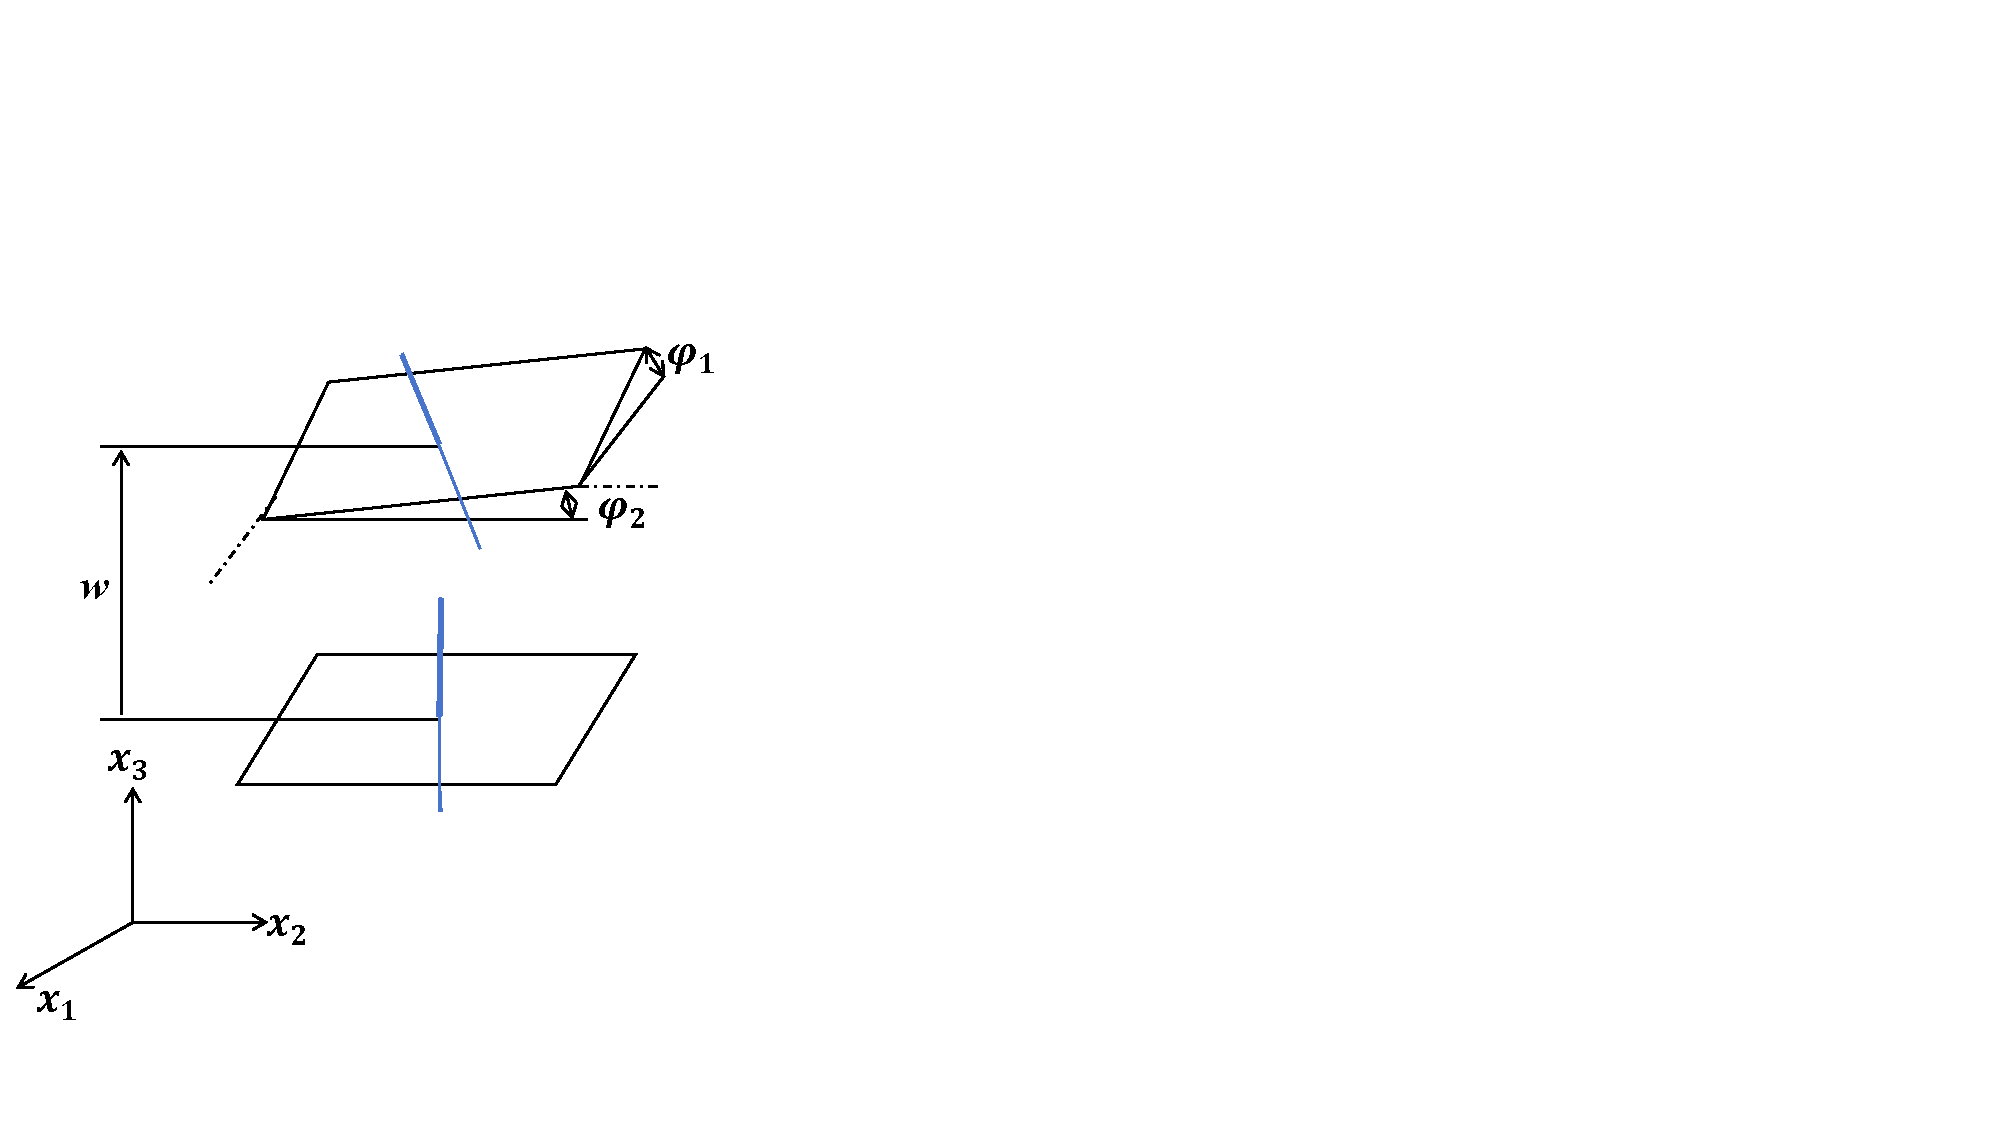
\includegraphics[width=2in]{CUMCMThesis-master/figures/11.pdf}%
\label{fig_first_case}}
\hfil
\subfloat[右平面方向法线位移示意图]{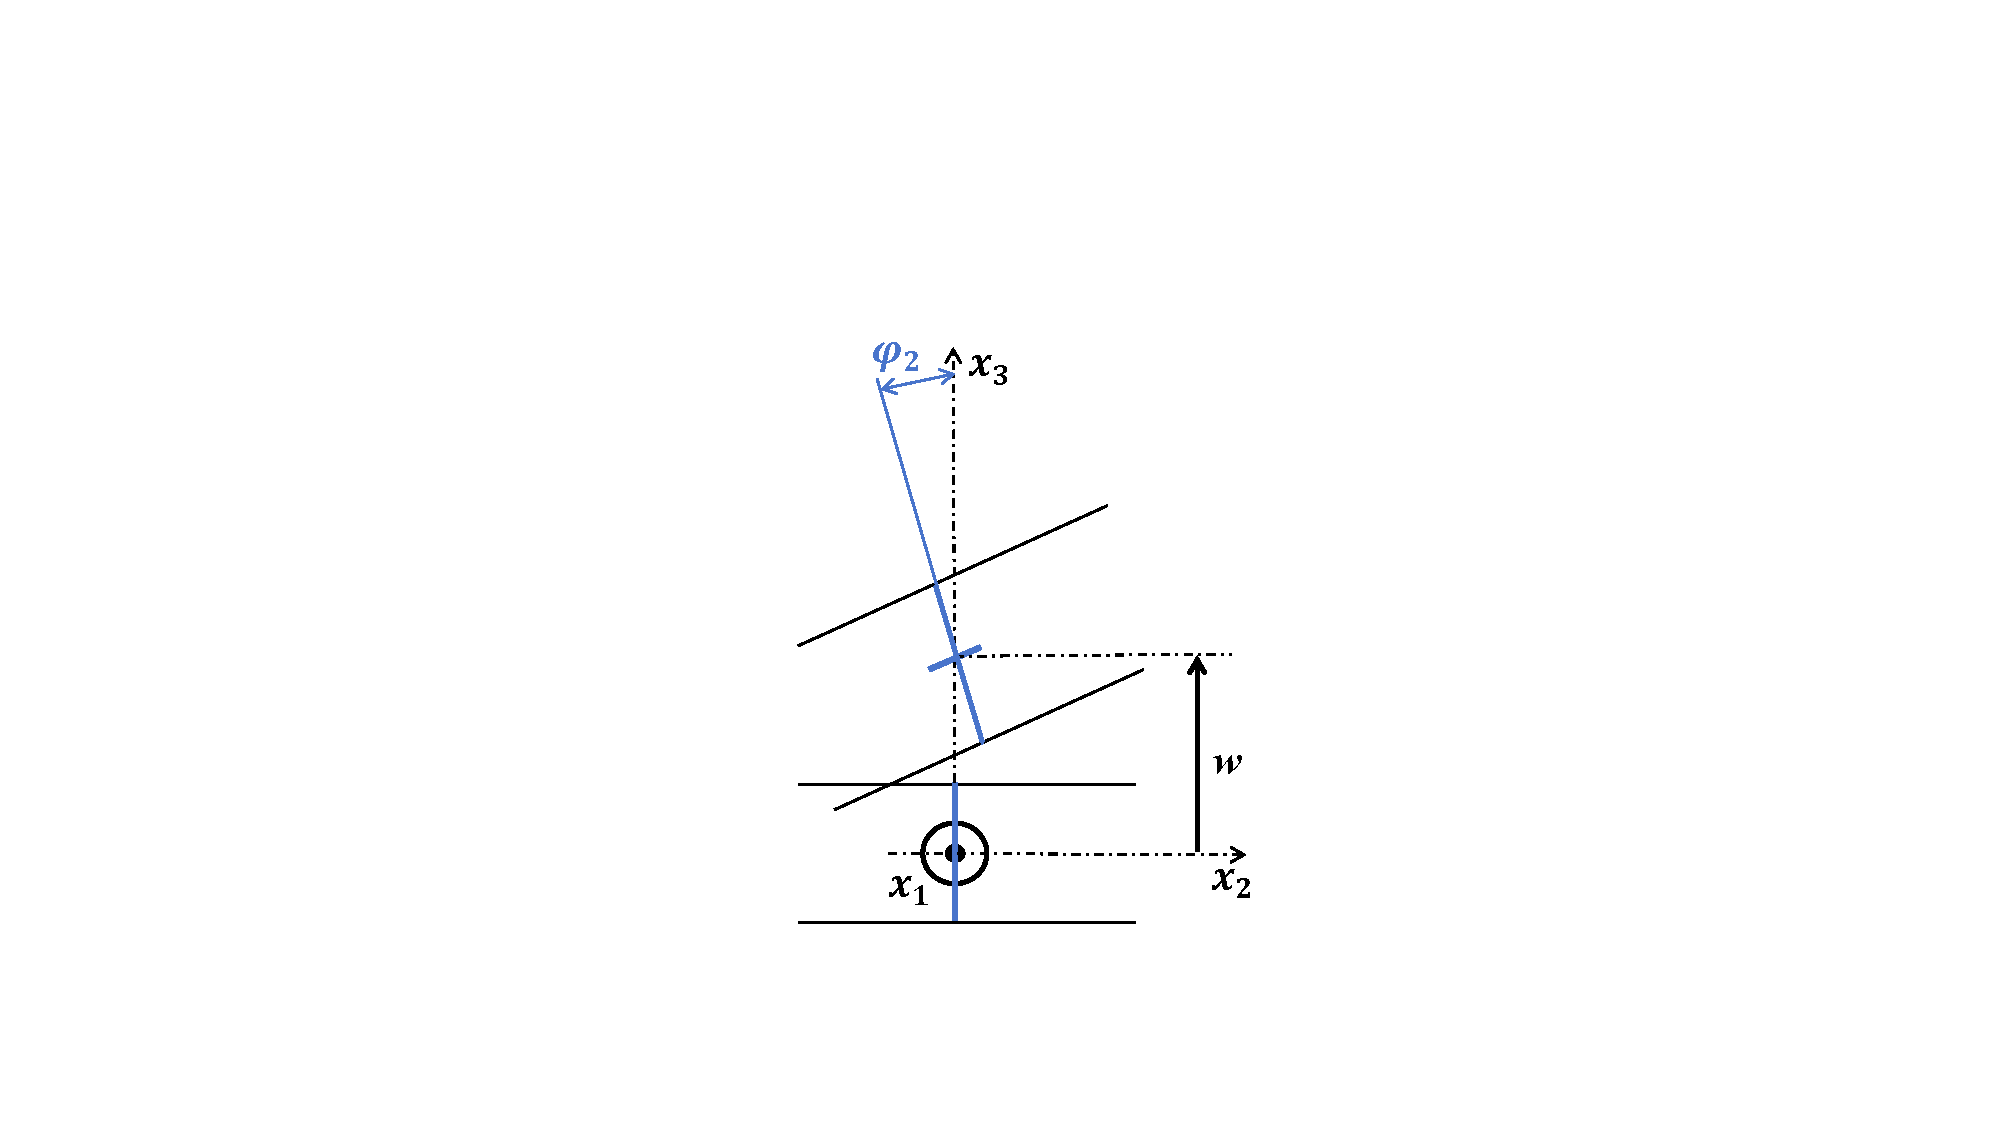
\includegraphics[width=2in]{CUMCMThesis-master/figures/12.pdf}%
\label{fig_second_case}}
\subfloat[左平面方向法线位移示意图]{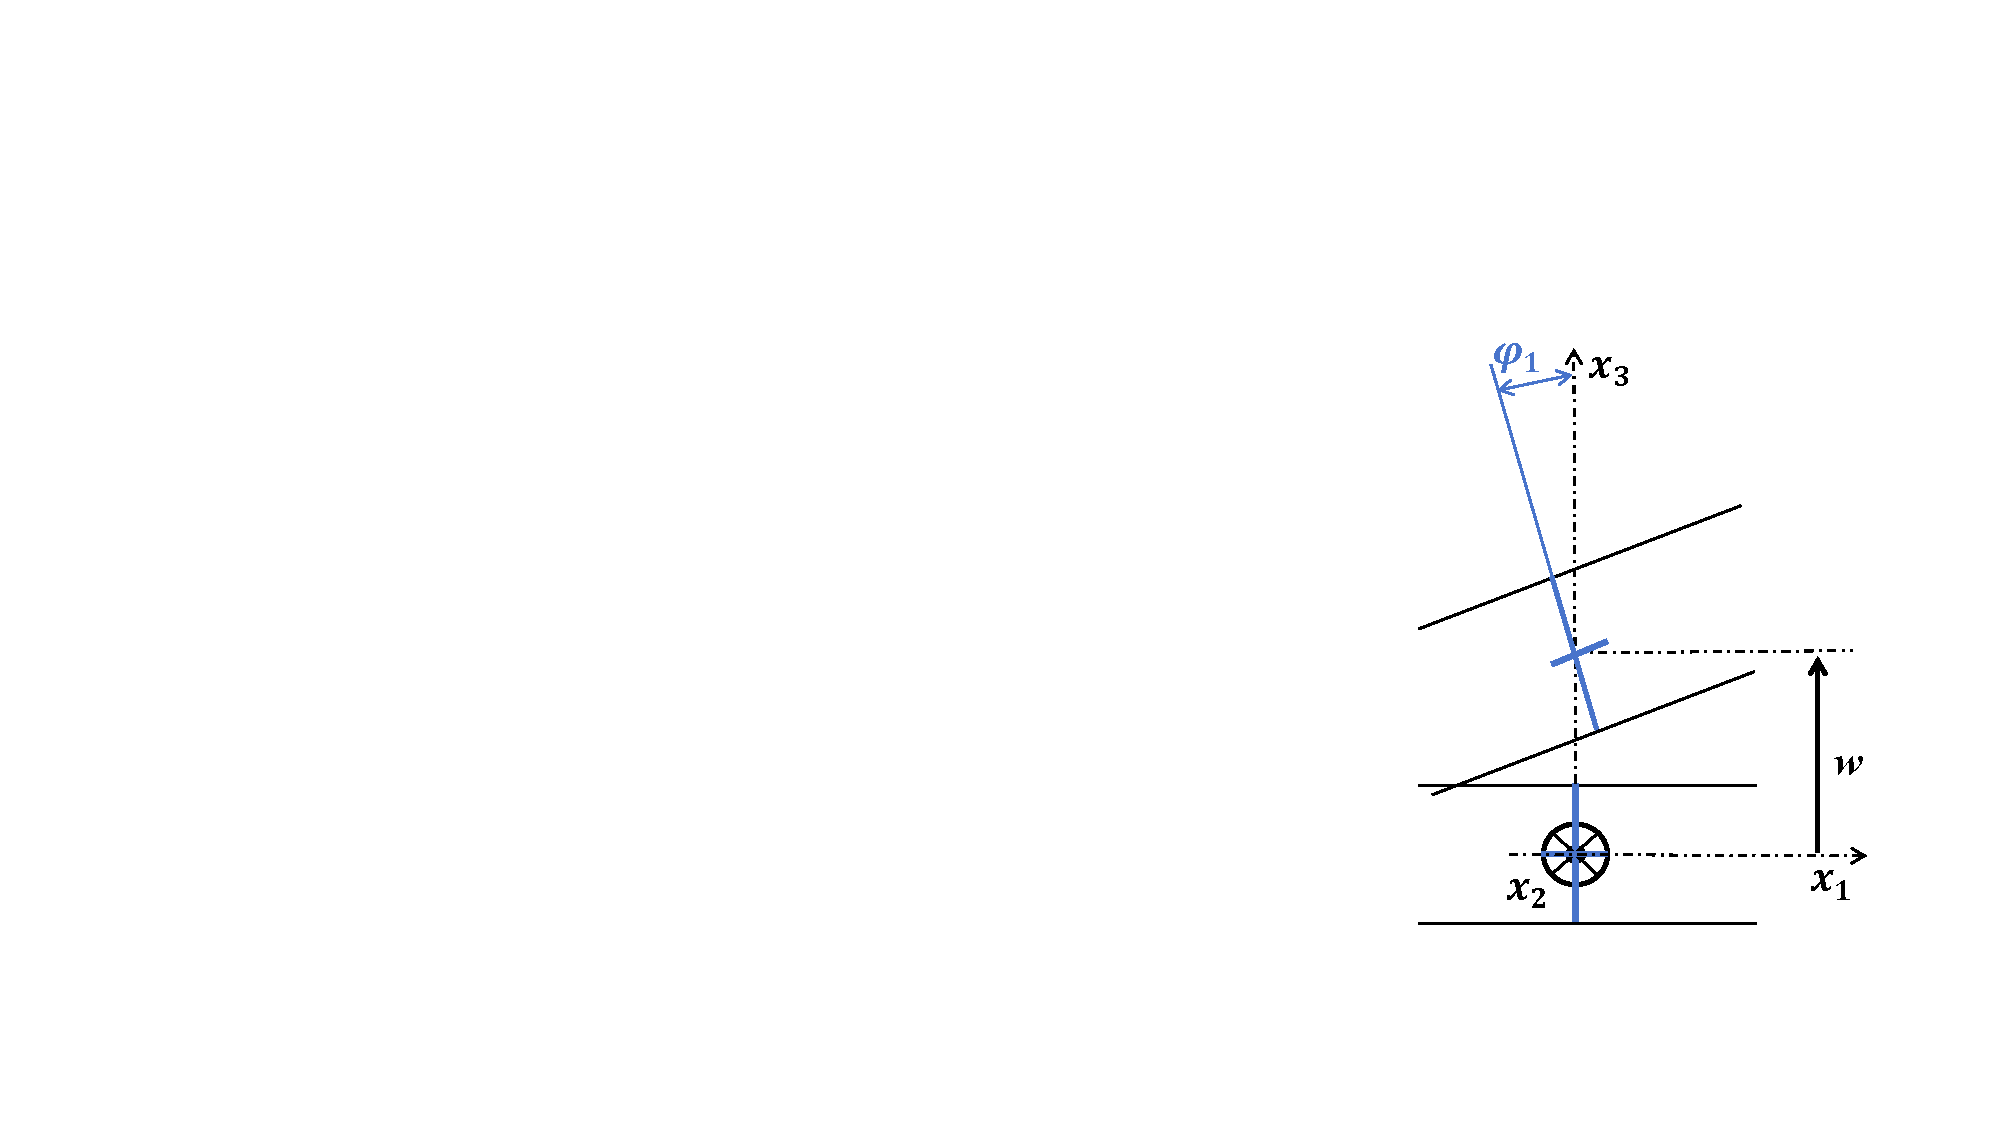
\includegraphics[width=2in]{CUMCMThesis-master/figures/13.pdf}%
\label{fig_third_case}}
\caption{平面位移示意图}
\label{fig_1}
\vspace{-0.4cm}
\end{figure*}
\subsubsection{形变-应力关系}
为保证可读性,本节之中使用符号说明如表~\ref{table-2}~所示。
\begin{table}[H]
	\caption{\textbf{3.1.2节符号说明}}%title
	\centering
	\begin{tabular}{ll}% four columns
		\hline %begin the first line
		符号   &  含义  \\
		\hline %begin the second line
		$\varepsilon_{\alpha\beta}$ &平面应变量\\
		$\delta W_{ext}$&外力的虚拟功\\
		$\delta W_{int}$&内力的虚拟功\\
		$q(x)$&分布载荷\\
		$\delta w$&垂直方向上得到虚拟位移\\
		$h$	&板厚度的一半\\
		$\sigma_{\alpha\beta}$&板受到的压力\\
		$N_{\alpha\beta,\alpha}$&应力合力\\
		$M_{\alpha\beta,\alpha}$&应力矩合力\\
		\hline %begin the third line
	\end{tabular} \label{table-2}
\end{table}
利用~\eqref{2}~建立起的形变坐标表达式,可定义因震动导致的变形与弯曲的平面应变:
\begin{equation}
    \begin{aligned}
&\varepsilon_{\alpha\beta}=\frac{1}{2}\left(\frac{\partial U_\alpha}{\partial x_{\beta}}+\frac{\partial U_{\beta}}{\partial x_\alpha}\right)\equiv\frac{1}{2}\left(U_{\alpha,\beta}+U_{\beta,\alpha}\right)\\
&\varepsilon_{\alpha3}=\frac{1}{2}\left(\frac{\partial U_\alpha}{\partial x_{3}}+\frac{\partial U_{\beta}}{\partial x_\alpha}\right)\equiv\frac{1}{2}\left(U_{\alpha,3}+U_{3,\alpha}\right)\\
&\epsilon_{33}=\frac{\partial U_3}{\partial x_3}\equiv U_{33}~;~\alpha,\beta=1,2,
    \label{3}\end{aligned}
\end{equation}
利用2.1.1节中的运动学假设,对~\eqref{3}~进行进一步计算,可以得到:
\begin{equation}
	\begin{aligned}
&\varepsilon_{\alpha\beta}=\frac{1}{2}(U^0_{\alpha,\beta}+U^0_{\beta,\alpha})-x_{3}w^0_{\alpha\beta}\\
		&\varepsilon_{\alpha3}=-w^0_{\alpha}+w^0_{\alpha}=0\\
		&\varepsilon_{33}=0 ~;~\alpha,\beta=1,2,
	\end{aligned}\label{4}
\end{equation}
因$\epsilon_{33}=0$,所以唯一的非零应变量为平面应变量。

在得到平面应变量$\varepsilon_{\alpha\beta}$后,基于能量平衡原理计算薄板的受力情况。为保证模拟的可靠性,在这一部分之中采用基于变分理论的虚功原理来进行计算,利用2.1.2节的虚拟位移假设,有虚功定理表达式:
\begin{equation}
    \delta W_{ext}=\delta W_{int},\label{5}
\end{equation}
其中$\delta W_{ext}$是外力的虚拟功,$\delta W_{int}$是内力的虚拟功。

分布载荷$q(x)$指向$x_3$方向的虚拟功表示为:
\begin{equation}
    \delta W_{ext}=\int_A q(x)\delta wdA,\label{6}
\end{equation}
其中$\delta w$是垂直方向上得到虚拟位移。

将~\eqref{3},\eqref{4},\eqref{5}~式带入~\eqref{6}~可以得到板的平衡方程:
\begin{equation}
    \begin{aligned}
        &\frac{\partial N_{\alpha\alpha}}{\partial x_\alpha}+\frac{\partial N_{\beta\alpha}}{\partial x_\beta}=0\\
        &\frac{\partial N_{\alpha\beta}}{\partial x_\alpha}+\frac{\partial N_{\beta\beta}}{\partial x_\beta}=0\\
        &\frac{\partial^2M_{\alpha\alpha}}{\partial x_\alpha^{2}}+2\frac{\partial^2 M_{\alpha\beta}}{\partial x_\alpha \partial x_\beta}+\frac{\partial^2 M_{\beta\beta}}{\partial x_\beta^2}=-q.
    \end{aligned}\label{7}
\end{equation}

若板的厚度记为$2h$,$\sigma_{\alpha\beta}$表示板受到的压力,则~\eqref{7}~式中不同的$N,M$表示为:
\begin{equation}
    \begin{aligned}
        N_{\alpha\beta,\alpha}&=0\quad N_{\alpha\beta}\coloneqq\int_{-h}^{h}\sigma_{\alpha\beta}dx_3\\
        M_{\alpha\beta,\alpha\beta}+q&=0\quad M_{\alpha\beta}\coloneqq\int_{-h}^{h}x_3\sigma_{\alpha\beta}dx_3.
    \end{aligned}\label{8}
\end{equation}

为更好描述~\eqref{7}~式中不同的$N$,$M$的力矩与应力几何关系,现将示意图整理如图~\ref{2}~所示。
\begin{figure*}[htbp]
\centering
\subfloat[弯矩和法向应力]{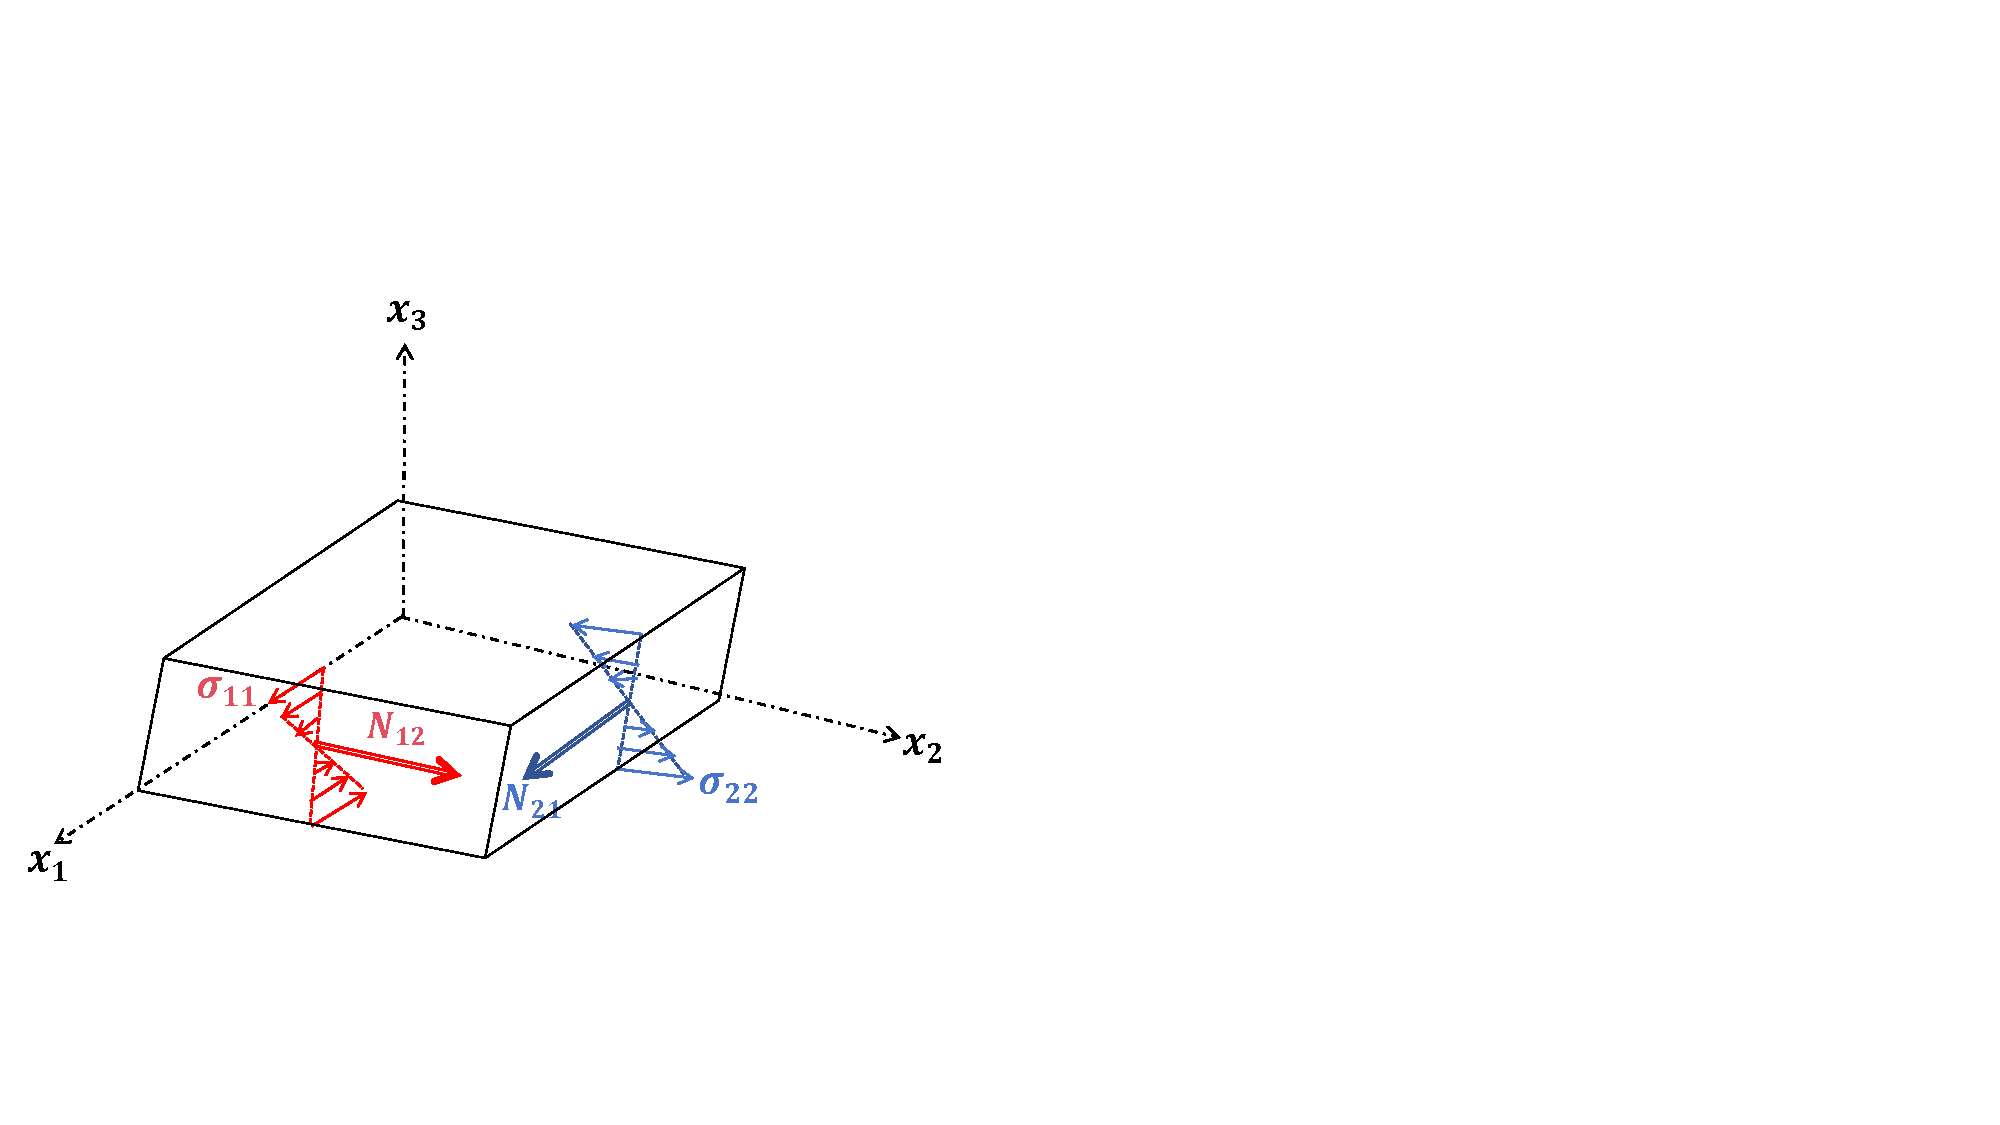
\includegraphics[width=2in]{CUMCMThesis-master/figures/21.pdf}%
\label{fig_first_case}}
\hfil
\subfloat[扭矩和剪切应力]{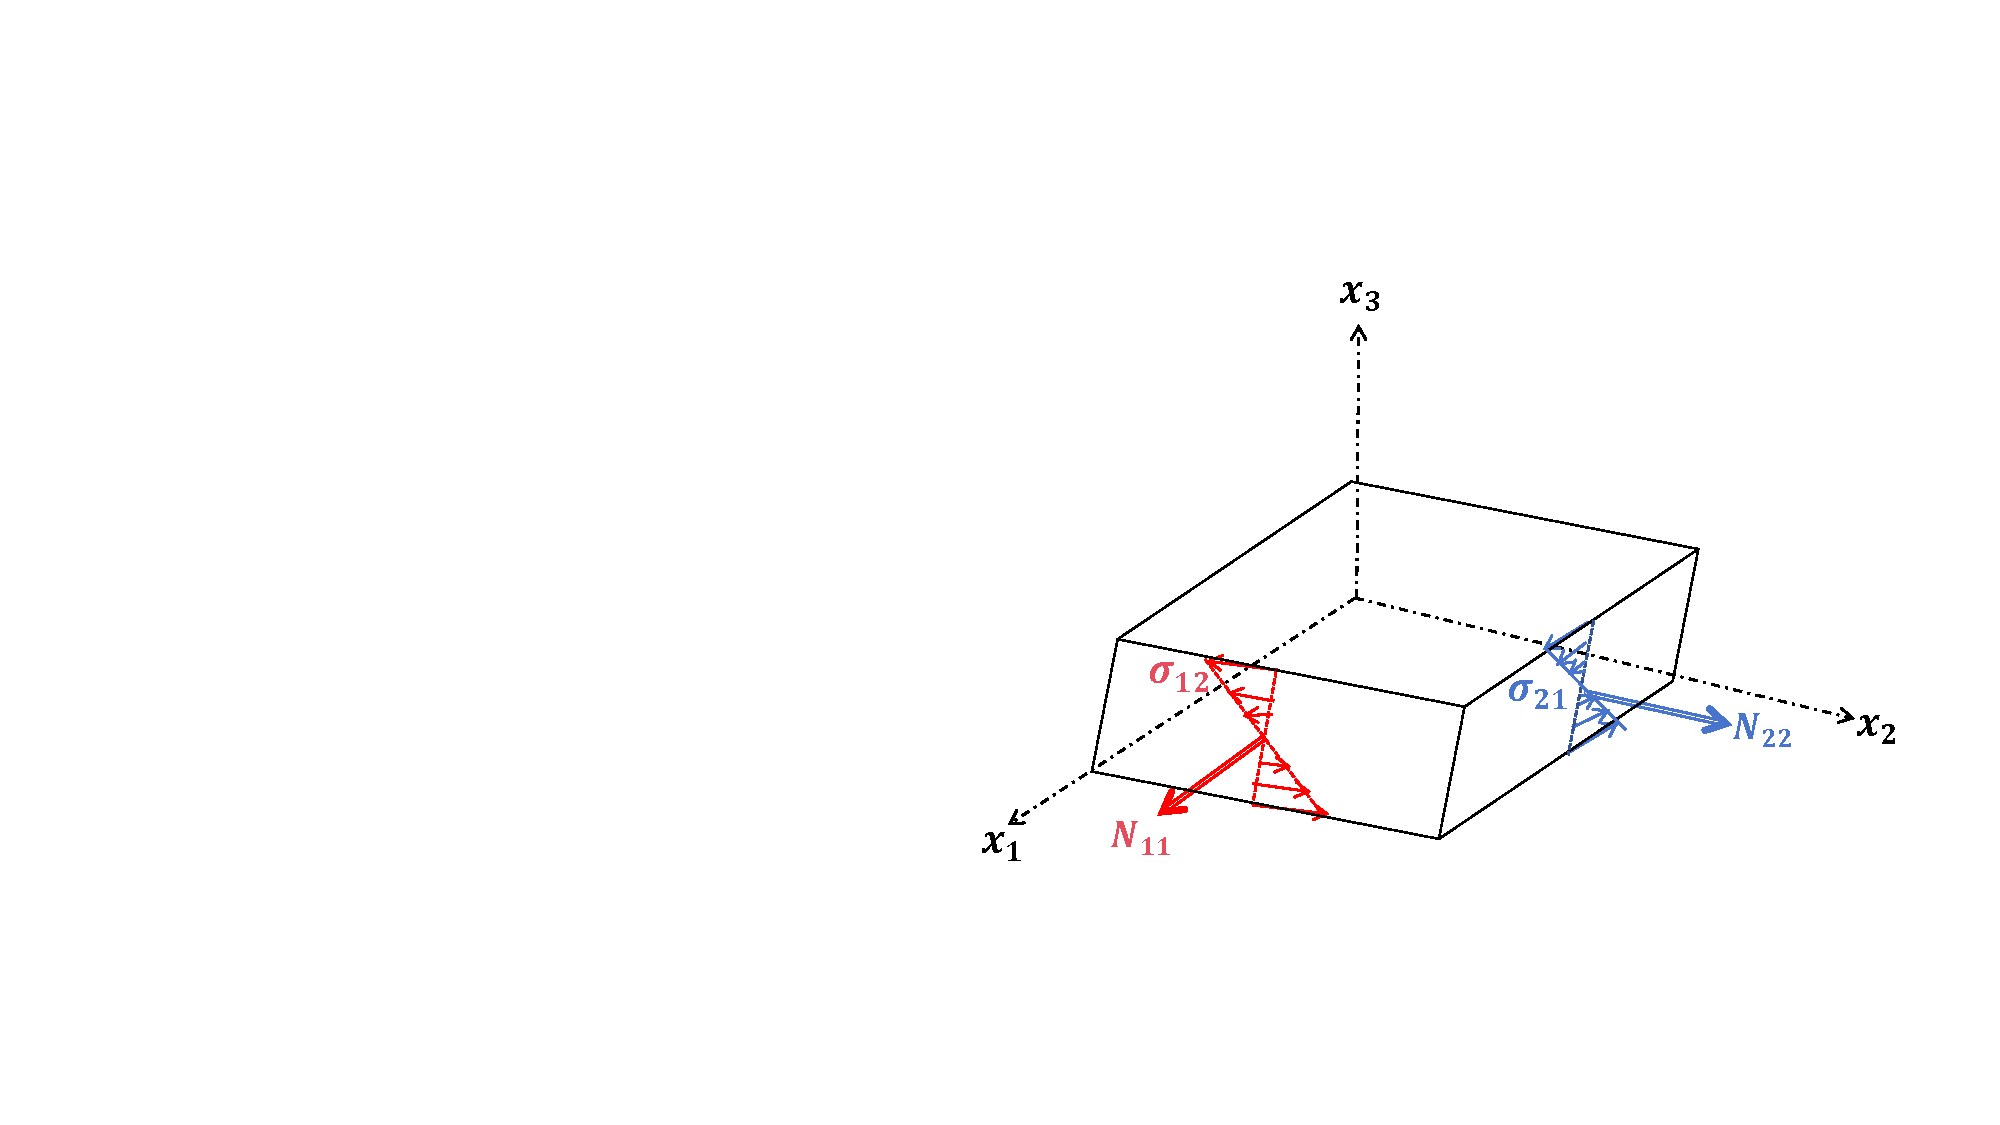
\includegraphics[width=2in]{CUMCMThesis-master/figures/22.pdf}%
\label{fig_second_case}}
\caption{力矩与应力的几何示意图}
\label{fig_2}
\vspace{-0.4cm}
\end{figure*}
\subsubsection{应力偏微分方程求解}
为保证可读性,本节之中使用符号说明如表~\ref{table-3}~所示。
\begin{table}[H]
	\caption{\textbf{3.1.3节符号说明}}%title
	\centering
	\begin{tabular}{ll}% four columns
		\hline %begin the first line
		符号   &  含义  \\
		\hline %begin the second line
		$C$&弹性矩阵\\
		$\epsilon$&应变张量\\
		$G$&剪切模量\\
		$E$&弹性模量\\
		$v$&泊松比\\
		$Q$&剪力\\
		\hline %begin the third line
	\end{tabular} \label{table-3}
\end{table}
广义胡克定律可以用已知应力求未知应变,其数学表达式为:
\begin{equation}
    \begin{aligned}
     &\epsilon_{\alpha\alpha}=\frac{1}{E}\left[\sigma_{\alpha\alpha}-v\left(\sigma_{\beta\beta}+\sigma_{33}\right)\right]~,~\epsilon_{\beta3}=\frac{1}{G}\sigma_{\beta3}\\
     &\epsilon_{\beta\beta}=\frac{1}{E}\left[\sigma_{\beta\beta}-v\left(\sigma_{33}+\sigma_{\alpha\alpha}\right)\right]~,~\epsilon_{3\alpha}=\frac{1}{G}\sigma_{3\alpha}\\
     &\epsilon_{33}=\frac{1}{E}\left[\sigma_{33}-v\left(\sigma_{\alpha\beta}+\sigma_{\beta\beta}\right)\right]~,~\epsilon_{\alpha\beta}=\frac{1}{G}\sigma_{\alpha\beta},
    \end{aligned} \label{9}
\end{equation}
\eqref{9}~中$G$是剪切模量,$E$为弹性模量,$v$为泊松比。并且$G$能由$E$,$v$表示:
\begin{equation}
\begin{aligned}
    G=\frac{E}{2(1+v)}, \label{10}
\end{aligned}    
\end{equation}
对~\eqref{9},\eqref{10}~联立求解,可以得到进一步的应力应变关系式为:
\begin{equation}
    \begin{aligned}
        \sigma_{\alpha\alpha}&=E\frac{\epsilon_{\alpha\alpha}+v\epsilon_{\beta\beta}}{1-v^2}\\
        \sigma_{\beta\beta}&=E\frac{\epsilon_{\beta\beta}+v\epsilon_{\alpha\alpha}}{1-v^2}\\
        \sigma_{\alpha\beta}&=G\epsilon_{\alpha\beta}.
    \end{aligned}\label{11}
\end{equation}

在求解动力方程前,提前给出动力方程的边界条件。在求解板理论平衡方程所需的边界条件可以从虚功原理中的边界项中得到,在边界没有外力的情况下,边界条件:
\begin{equation}
    \begin{aligned}
     n_\alpha N_{\alpha\beta} &~\text{或}~U_\beta^0\\
     n_\alpha M_{\alpha\beta,\beta} &~\text{或}~w^0\\
     n_\beta M_{\alpha\beta}&~\text{或}~w_\alpha^0.
    \end{aligned}\label{12}
\end{equation}

若考虑自由边界情况,则边界条件进一步简化为$M=0;Q=0$。其中$M$代表弯矩,$Q$代表剪力。现可以将已有的条件带入~\eqref{5}~计算由弯矩与剪力表示的的虚拟功$\delta W_{int}$:
\begin{equation}
    \begin{aligned}
        \delta W_{int}=\int_A\left(M_{\alpha\alpha}\delta k_{\alpha\alpha}+M_{\beta\beta}\delta k_{\beta\beta}+M_{\alpha\beta}\delta k_{\alpha\beta}\right),
    \end{aligned}\label{13}
\end{equation}
\eqref{13}~式中出现的$k$的表达式为:
\begin{equation}
    \begin{aligned}
        k_{\alpha\alpha}&=\frac{\partial^2w}{\partial x_\alpha^2}\\
        k_{\beta\beta}&=\frac{\partial^2w}{\partial x_\beta^2}\\
        k_{\alpha\beta}&=\frac{\partial^2w}{\partial x_{\alpha\beta}}.
    \end{aligned}\label{14}
\end{equation}

将~\eqref{7},\eqref{8},\eqref{9},\eqref{10},\eqref{11},\eqref{14}~带入~\eqref{13}~中,可以得到:
\begin{equation}
        \delta W_{int}=\int_A\left(D\frac{\partial^2 w^0}{\partial x_{\alpha}^2}\delta\frac{\partial^2w^0}{\partial x_{\alpha}^2}+D\frac{\partial^2w^0}{\partial x_{\beta}^2}\delta\frac{\partial^2w^0}{\partial x_{\beta}^2}+4D\frac{\partial^2w^0}{\partial x_{\alpha}x_{\beta}}\delta\frac{\partial^2w^0}{\partial x_{\alpha}x_{\beta}}\right)dA\label{15}.
\end{equation}

对~\eqref{14}~使用变分法,可以得到:
\begin{equation}
    \begin{aligned}
        \delta 
 k_{\alpha\alpha}&=\frac{\partial^2 \delta w}{\partial x_\alpha^2}\\
         \delta k_{\beta\beta}&=\frac{\partial^2 \delta w}{\partial x_\beta^2}\\
         \delta k_{\alpha\beta}&=\frac{\partial^2 \delta w}{\partial x_\alpha x_\beta}.
    \end{aligned}\label{16}
\end{equation}

将~\eqref{16}~的结果带入~\eqref{15}~中,可以得到全新的内力虚拟功表达式:
\begin{equation}
        \delta W_{int}=D\int_A\left(\frac{\partial^2w^0}{\partial x_{\alpha}^2}\frac{\partial^2\delta w^0}{\partial x_{\alpha}^2}+\frac{\partial^2w^0}{\partial x_{\beta}^2}\frac{\partial^2\delta w^0}{\partial x_{\beta}^2}+4\frac{\partial^2w^0}{\partial x_{\alpha}x_{\beta}}\frac{\partial^2\delta w^0}{\partial x_{\alpha}x_{\beta}}\right)dA.\label{17}
\end{equation}

把~\eqref{6},\eqref{17}~带入等式~\eqref{5}~中,可以得到最终的虚功积分方程:
\begin{equation}
        \int_A q(x)\delta wdA=D\int_A\left(\frac{\partial^2 w^0}{\partial x_{\alpha}^2}\frac{\partial^2\delta w^0}{\partial x_{\alpha}^2}+\frac{\partial^2w^0}{\partial x_{\beta}^2}\frac{\partial^2\delta w^0}{\partial x_{\beta}^2}+4\frac{\partial^2w^0}{\partial x_{\alpha}x_{\beta}}\frac{\partial^2\delta w^0}{\partial x_{\alpha}x_{\beta}}\right)dA.\label{18}
\end{equation}

对~\eqref{18}~进行分部积分,并带入~\eqref{12}~的边界条件,可以得到最终的控制方程:
\begin{equation}
    D\bigtriangleup^4w^0+\rho h=q(x). \label{19}
\end{equation}
若没有外部载荷,则~\eqref{20}~退化为:
\begin{equation}
        D\bigtriangleup^4w^0+\rho h=0, \label{20}
\end{equation}
式~\eqref{20}~通过简化三维弹性力学方程,提供一个有效的框架来分析和计算薄板的振动模态。这使得在后续部分能够高效地解决板振动问题。
\subsection{分析问题一:弹力学方程求解}
为保证可读性,本节之中使用符号说明如表~\ref{table-4}~所示。
\begin{table}[!htbp]
	\caption{\textbf{3.2节符号说明}}%title
	\centering
	\begin{tabular}{ll}% four columns
		\hline %begin the first line
		符号   &  含义  \\
		\hline %begin the second line
	$\rho$&密度\\
	$D$&弯曲挠度\\
	$T(t)$&时间方程\\
	$W(x,y)$&空间方程\\
	$\lambda$&分离常数因子\\
	$r$&特征根\\
	$\omega$&角频率\\
		\hline %begin the third line
	\end{tabular}\label{table-4}
\end{table}
对于不均匀的薄板震动问题,依然可以应用基尔霍夫-洛夫理论进行分析。但需要考虑材料参数是建立在三维位移空间下的函数。但这样的分析过于复杂,现引用2.2.3节中不均匀模板假设,并解释假设依据~\cite{ref3}\cite{ref4}。

\subsubsection{连续性假设与分离变量法}
对于不均匀薄板,可以考虑材料参数是基于空间坐标的函数。分别将密度$\rho$和弯曲挠度$D$分别表示为:$\rho\left(x_{\alpha},x_{\beta},x_3\right)D\left(x_{\alpha},x_{\beta},x_3\right)$。但三维偏微分方程求解的计算量和难度过大,考虑到本题是对现实之中的物体建模,则给出连续性假设:现实中的物体轮廓往往是连续函数。所以给出2.2.3节中的连续性假设。借助此假设,将$\rho,D$的函数转化为:
\begin{equation}
\begin{aligned}
&\rho\left(x_{\alpha},x_{\beta},x_3\right)=\rho\left(x_\alpha,x_\beta\right)\\&D\left(x_{\alpha},x_{\beta},x_3\right)=D\left(x_\alpha,x_\beta\right)=\frac{E\left(x_\alpha,x_\beta\right)h^3}{12\left(1v\left(x_\alpha,x_\beta\right)^2\right)}. 
    \end{aligned}
    \label{21}
\end{equation}

把~\eqref{21}~带入~\eqref{19}~可进一步建立不均匀薄板的基本方程:
\begin{equation}
\bigtriangleup\cdot\left(D\left(x,y\right)\bigtriangleup^2w^0\right)+\rho\left(x_\alpha,x_\beta\right)h\frac{\partial^2w^0}{\partial t^2}=0.
\label{22}\end{equation}

接下来,将使用分离变量法对~\eqref{22}~求解。首先将位移表示为空间与时间部分的乘积形式:
\begin{equation}
    w^0=w^0\left(x_\alpha,x_\beta,t\right)=W\left(x,y\right)\cdot T\left(t\right).\label{23}
\end{equation}

将~\eqref{23}~带入控制方程~\eqref{22}~可以得到分离变量方程:
\begin{equation}
    \bigtriangleup\cdot\left(D\left(x,y\right)\bigtriangleup^2W\left(x,y\right)\right)T\left(t\right)=-\rho\left(x_\alpha,x_\beta\right)hW\left(x_\alpha,x_\beta\right)\frac{\partial^2 T(t)}{\partial t^2},\label{24}
\end{equation}
对~\eqref{24}~两边同时除去多项式$W\left(x_{\alpha},x_{\beta}\right)T(t)$能得到分离变量后的两个微分方程:
\begin{align}
    \frac{d^2 T(t)}{dt}+\lambda T(t)&=0\label{25} \\
    \bigtriangleup\cdot\left(D\left(x_\alpha,x_\beta\right)\delta^2W\left(x_\alpha,x_\beta\right)\right)&=-\lambda\rho\left(x_{\alpha},x_{\beta}\right)hW\left(x_{\alpha},x_{\beta}\right),\label{26}
\end{align}
式~\eqref{25}~是时间部分的常微分方程,式~\eqref{26}~是空间部分的偏微分方程。$\lambda$的数学含义将在3.2.2节~\eqref{27}~给出具体说明。


\subsubsection{时域常微分方程求解}
通过分离参数得到的~\eqref{25}~的常微分模型并不受薄板本身性质干扰,对时域常微分的方程求解是通用于问题一问题二的步骤。而具体的求解步骤要通过前一部分的分离参数法~\eqref{25}\eqref{26}~来考虑。在这里给出分离常数因子$\lambda$的解释。

在分离变量时~\eqref{24}~同时除掉多项式因子时,有:
\begin{equation}
    \frac{\bigtriangleup\cdot\left(D\left(x_\alpha,x_\beta\right)\bigtriangleup W\left(x_\alpha,x_\beta\right)\right)}{W\left(x_\alpha,x_\beta\right)} = -\frac{\rho\left(x_\alpha,x_\beta\right)}{T(t)}\frac{\partial^2 T(t)}{\partial t^2}, \label{27}
\end{equation}
这其中左式作为$x_\alpha$,$x_\beta$的函数,右式为$t$的函数,若等式成立,则一定成立一个常数交点。这样的常数点被称为分离常数因子$\lambda$。

在普通的微分方程之中,分离常数因子仅作为求解使用,但在薄板模型的动力学微分方程中,分离常数因子作为重要的数学参数可以大幅度简化振动问题的计算方式。接下来将重点描述$\lambda$的意义,下面对~\eqref{25}~求解。

利用特征方程法求解,设解的形式为$T(t)=e^{rt}$则有特征方程:
\begin{equation}
    r^2e^{rt}+\lambda e^{rt}=0, \notag
\end{equation}
对二次方程求解可以得到特征根$r=\pm i\sqrt{\lambda}$,所以~\eqref{25}~的通解为:
\begin{equation}
    T(t)=A\cos(\omega t)+B\sin(\omega t)~,~\omega=\sqrt{\lambda}, \label{28}
\end{equation}
这表示薄板以角频率$\omega$进行简谐振动时,特征值$\lambda$代表对应频率的平方。通过求解时间部分的微分方程即可求得系统的自由振动解。而$\lambda$可以通过特征值分解的办法进行求解。
\subsection{分析问题一:经典边界条件下的固有振型分析}
相较于其他的边界条件而言,分析自由薄板的自由边界条件下的振型是较为复杂的,幸运地是目前已经有一些成熟的近似求解方案去求解自由薄板在自由边界条件下的固有振型。

在本节之中将介绍两种种经典应用于各向同性薄板的固有振型近似求法:视弹性耦合法与瑞雷法。
\subsubsection{视弹性耦合法求解固有振型}
结合~\eqref{4}~\eqref{8}~\eqref{11}~的数学式与细长杆理论,自由边界的矩形薄板的频率方程可表示为:
\begin{equation}
    \begin{aligned}
        &\tan [\omega L /(2V_{\alpha\alpha})]=\pm th \{\omega L/(2V_{\alpha\alpha})\}\\
        &\tan [\omega L /(2V_{\beta\beta})]=\pm th \{\omega L/(2V_{\beta\beta})\}
    \end{aligned}
\end{equation}
进一步求解可得到:
\begin{equation}
    f_1=\frac{2CR_{\alpha\alpha} P^2(i)}{\pi L^2\sqrt{1-v^2}},f_2=\frac{2CR_{\beta\beta} P^2(j)}{\pi L^2\sqrt{1-v^2}}
\end{equation}
其中$i,j$分别代表两个方向的模态,最终得到的频率指标为:
\begin{equation}
    f_{ij}=\sqrt{f_{i\alpha\alpha}^2+f_{j\beta\beta}^2}
\end{equation}
\subsubsection{瑞雷法求解固有振型}
相较于上一种方法的特殊性,瑞雷法是在薄板振动领域之中更常用的方法。

瑞雷提出一个目前广为利用的确定震动体系最低固有振型的近似方法。这是假定与振型相近的形变函数带入位移变分原理的计算公式。对于平板,可取给定的位移边界条件的振型近似函数:
\begin{equation}
    W(\alpha,\beta)=A_1W_1(\alpha,\beta)
\end{equation}
其中$A_1$是任意常数,$W_1(\alpha,\beta)$为选定的版面坐标的函数。代入位移变分原理式可以得到:
\begin{equation}
\begin{aligned}
        \delta [U_m-\omega^2 T_m]&=\delta\{A_1^2[U_m(W_1)-\omega^2T_m(W_1)]\}\\
        &=2A_1[U_m(W_1)-\omega^2 T_m(W_1)]\delta A_1=0
\end{aligned}
\end{equation}
又由于$A_1$的任意性,得到:
\begin{equation}
    U_m(W_1)-\omega^2T_m(W_1)=0
\end{equation}
在此式的基础上,即有$\omega^2=\dfrac{U_m(W_1)}{T_m(W_1)}$
\subsection{分析问题二:极坐标系下的薄板振动方程}
针对于第二问之中的曲线边界板,使用直角坐标系进行计算将会使问题变得极其困难。此时使用极坐标将会大大减少问题的复杂度。此时位移$u$沿$r$方向,$v$沿$\theta$方向,$w$沿$z$方向。此时挠曲函数变为$w(r,\theta,t)$。利用圆柱坐标系的几何方程,可解得位移分量:
\begin{equation}
    \begin{aligned}
        u(r,\theta,z,t)&=-z\dfrac{\partial w(r,\theta,t)}{\partial r}\\
        v(r,\theta,z,t)&=-z\dfrac{\partial w(r,\theta,t)}{\partial \theta}
    \end{aligned}
\end{equation}    
进一步求应变分量:
	\begin{equation}
        \begin{aligned}
	\varepsilon_r&=\frac{\partial u}{\partial r}=-z\frac{\partial^2w}{\partial r^2}=-z\kappa_r\\       
	\varepsilon_\theta&=\frac{u}{r}+\frac{\partial v}{r \partial\theta}=-z(\frac{\partial w }{r\partial r}+\frac{\partial^2 w}{r^2 \partial \theta^2})=-z\kappa_\theta\\
	\gamma_{r\theta}&=\frac{\partial v}{r\partial \theta}+\frac{\partial v}{\partial r}-\frac{v}{r}=-2z\frac{\partial}{\partial r}(\frac{\partial w}{r \partial \theta})=-2z\kappa_{r\theta}
           \end{aligned}
		\end{equation}
弹性体动力学的圆柱坐标系物理方程有:
	\begin{equation}
		\begin{aligned} 
			&\varepsilon_r=\frac{1}{E}(\sigma-\nu\sigma_\theta)\\
			&\varepsilon_\theta=\frac{1}{E}(\sigma_\theta-\nu\sigma_r)\\
			&\gamma_{r\theta}=\frac{\tau_{r\theta}}{G}\\
		\end{aligned}
	\end{equation}
	解出应力分量,带入应变表达式有:
	\begin{equation}
 \begin{aligned}
		\sigma_r&=\frac{E}{1-\nu^2}(\varepsilon_r+\nu\varepsilon_\theta)=-\frac{E}{1-\nu^2}z[\frac{\partial^2w}{\partial r^2}+\nu(\frac{\partial w}{r\partial r}+\frac{\partial^2 w}{r^2\partial \theta^2})]\\
     \sigma_\theta&=\frac{E}{1-\nu^2}(\varepsilon_\theta+\nu\varepsilon_r)=-\frac{E}{1-\nu^2}z[(\frac{\partial w}{r\partial r}+\frac{\partial^2 w}{r^2\partial \theta^2})+\nu\frac{\partial^2 w}{\partial r^2}]\\
	\tau_{r\theta}&=G\gamma_{r\theta}=-2Gz\frac{\partial }{\partial r}(\frac{\partial w}{r \partial \theta})
  \end{aligned}
	\end{equation}

所以得到极坐标系内力分量:弯矩、扭矩、剪力的数学表达式为:
		\begin{equation}
        \begin{aligned}    
	M_r&=\int_{-\frac{h}{2}}^{\frac{h}{2}}\sigma_r zdz,\:\:\:M_\theta=\int_{-\frac{h}{2}}^{\frac{h}{2}}\sigma_\theta zdz,\:\:\:M_{r\theta}=\int_{-\frac{h}{2}}^{\frac{h}{2}}\tau_{r\theta} zdz\\
	Q_r&=\int_{-\frac{h}{2}}^{\frac{h}{2}}\tau_{zr}dz,\:\:\:Q_\theta=\int_{-\frac{h}{2}}^{\frac{h}{2}}\tau_{\theta z}dz,
         \end{aligned}
	\end{equation}
	进一步计算可得可得弯矩,扭矩表达式:
		\begin{equation}
        \begin{aligned}    
		M_r&=-D[\frac{\partial^2 w}{\partial r^2}+\nu(\frac{\partial w}{r\partial r}+\frac{\partial^2w}{r^2\partial \theta^2})]\\   
		M_\theta&=-D[(\frac{\partial w}{r\partial r}+\frac{\partial^2w}{r^2\partial \theta^2})+\nu\frac{\partial^2 w}{\partial r^2}]\\
		M_{r\theta}&=-D(1-\nu)\frac{\partial}{\partial r}(\frac{\partial w}{r\partial \theta})        \end{aligned}
	\end{equation}
	
	根据薄板假设,忽略其惯性力矩有表达式:
	\begin{equation}	  
        \begin{aligned}
		&\frac{\partial M_r}{\partial r}+\frac{\partial M_{\theta r}}{r\partial \theta}-Q_r=0\\
	&\frac{\partial M_{r\theta}}{\partial r}+\frac{\partial M_{\theta}}{r\partial \theta}-Q_\theta=0\\
	&\frac{\partial Q_r}{\partial r}+\frac{\partial Q_\theta}{r\partial \theta}+q-\rho h\frac{\partial^2w}{\partial t^2}=0
         \end{aligned}
	\end{equation}
 
        将剪力方程互相联立,可得到:
 \begin{equation}
 \begin{aligned}
		Q_r&=-D\frac{\partial}{\partial r}\nabla^2w\\
		Q_\theta&=-D\frac{\partial}{r\partial\theta}\nabla^2w\\
   \end{aligned}
	\end{equation}
	式中$\nabla^2=(\frac{\partial^2}{\partial r^2}+\frac{\partial}{r\partial r}+\frac{\partial^2}{r^2\partial\theta^2})$为极坐标系的拉普拉斯算子。
	
	最终得到极坐标系中薄板横向振动的基本微分方程:
	\begin{equation}
		(\frac{\partial^2}{\partial r^2}+\frac{\partial }{r\partial r}+\frac{\partial^2}{r^2\partial \theta^2})(\frac{\partial^2 w}{\partial r^2}+\frac{\partial^2 w}{r\partial r^2}+\frac{\partial^2w}{r^2\partial\theta^2})+\frac{\rho h}{D}\frac{\partial^2w}{\partial t^2}=\nabla^2\nabla^2w+\frac{\rho h}{D}\frac{\partial^2w}{\partial t^2}=\frac{q}{D}(r,\theta,t)
	\end{equation}
	由此可知,极坐标系中薄板振动方程和直角坐标系中方程$(2.10)$在形式上是一样的,只要各自采用相应的拉普拉斯算子。
	
	如果板件形状、荷载及边界、初始条件均以平板中心轴对称,则挠曲函数$w$与$\theta$无关,这时有轴对称方程:
	\begin{equation}
		\begin{aligned} 
		\frac{\partial^4 w}{\partial r^4}+\frac{2\partial^8 w}{r\partial r^8}-\frac{\partial^2 w}{r^2\partial r^2}+\frac{\partial w}{r^8\partial r}+\frac{\rho h}{D}\frac{\partial^2 w}{\partial t^2}&=\frac{\partial}{r\partial r}\{r\frac{\partial}{\partial r}[\frac{\partial}{r\partial r}(r\frac{\partial w}{\partial r})]\}+\frac{\rho h}{D}\frac{\partial^2 w}{\partial t^2}\\
		&=\frac{q}{D}(r,t)
		\end{aligned} 
	\end{equation}
	而相应内力、应力、应变、位移表达式中含$\tfrac{\partial (\cdot)}{\partial\theta}$各项也均将消失。
 \subsection{分析问题二:正交各向异性的求解}
    针对复杂的各向异性体,一般采用线性应力-应变关系构造广义胡克矩阵表达式:
    \begin{equation}
        \begin{pmatrix}
\epsilon_{\alpha\alpha}\\
\epsilon_{\beta\beta}\\
\epsilon_{33}\\
\gamma_{\beta 3}\\
\gamma_{33}\\
\gamma_{\alpha 3}
\end{pmatrix}=
\begin{vmatrix}
a_{11}&a_{12}&a_{13}&a_{14}&a_{15}&a_{16}\\
a_{21}&a_{22}&a_{23}&a_{24}&a_{25}&a_{26}\\
a_{31}&a_{32}&a_{33}&a_{34}&a_{35}&a_{36}\\
a_{41}&a_{42}&a_{43}&a_{44}&a_{45}&a_{46}\\
a_{51}&a_{52}&a_{53}&a_{54}&a_{55}&a_{56}\\
a_{61}&a_{62}&a_{63}&a_{64}&a_{65}&a_{66}
\end{vmatrix} 
        \begin{pmatrix}
\sigma{\alpha\alpha}\\
\sigma_{\beta\beta}\\
\sigma_{33}\\
\tau_{\beta 3}\\
\tau_{33}\\
\tau_{\alpha 3}
\end{pmatrix}
    \end{equation}

    因薄板的正交各项异质体假设,有:
    \begin{equation}
        a_{14}=a_{15}=a_{16}=a_{24}=a_{25}=a_{26}=a_{34}=a_{35}=a_{36}=a_{46}=a_{56}==0
    \end{equation}
    故其控制基本方程变为:
    \begin{equation}
        D_{\alpha\alpha}\frac{\partial^4 \omega}{\partial \alpha^4}+2(D_{\alpha\alpha}v_{\alpha\beta}+2D_3)\frac{\partial^4\omega}{\partial \alpha^2 \partial \beta^2}D_{\beta\beta}\frac{\partial^4 \omega}{\partial \beta^4}+\rho h\frac{\partial^2 \omega}{\partial t^2}=q
    \end{equation}
    
假若材料具有横观各向同性材料构成,则有:
\begin{equation}
    D_\alpha=D_\beta=D_3;v_{\alpha\beta}=v_{\beta\alpha}=v
\end{equation}

则此时控制方程退化为:
\begin{equation}
    D\bigtriangleup^4w^0+\rho h=q(x). 
\end{equation}

在前一节之中已经构造了极坐标方程,所以直接将结果带入,得到最终的极坐标正交各向异性薄板的基本控制方程:
\begin{equation}
    D_r\frac{\partial^4 \omega}{\partial r^4}+2\frac{D_r}{r}\frac{\partial^3 \omega}{\partial r^3}-\frac{D_\theta}{r^2}\frac{\partial^2 \omega}{\partial r^2}+\frac{D_\theta}{r^3}\frac{\partial \omega}{\partial r}+\rho h \frac{\partial^2 \omega}{\partial t^2}=q
\end{equation}
\subsection{分析问题三:振型函数分解}
题目附件给出了通过特殊设备获得的某种具有自由边界条件非均质音板的5个模态情况,图片通过不同的颜色表达不同的振动方向与振幅大小。在没有直接提供数据的情况下,需要先提取图片之中隐藏的震动信息,在利用傅里叶变换等方式得到需要的振型函数。
\subsubsection{图片信息读取}
为保证可读性,本节之中使用符号说明如表~\ref{table-5}~所示。

\begin{table}[H]
	\caption{\textbf{3.3.1节符号说明}}%title
	\centering
	\begin{tabular}{ll}% four columns
		\hline %begin the first line
		符号   &  含义  \\
		\hline %begin the second line
		$R$&红色亮度\\
		$G$&绿色亮度\\
		$B$&蓝色亮度\\
	    $H$&色调\\
	    $S$&饱和度\\
	    $V$&明度\\
		\hline %begin the third line
	\end{tabular}\label{table-5}
\end{table}
RGB色彩模式是工业界的一种颜色标准,是通过对红(R)、绿(G)、蓝(B)三个颜色通道的变化以及它们相互之间的叠加来得到各式各样的颜色的,RGB代表红、绿、蓝三个通道的颜色。

如果要直观的判断出音板的振动幅度,需要得到各个模态中不同色调的颜色深浅,此时,我们需要转换颜色空间RGB为HSV,从而得到音板各处的色调,饱和度以及亮度。

HSV(Hue, Saturation, Value)是根据颜色的直观特性创建的一种颜色空间,其中三种参数表示如下:
\begin{itemize}
	\item 色调\textbf{H}的取值范围为0$\sim$360°,从红色开始按逆时针方向计算,红色为0°,绿色为120°,蓝色为240°。它们的补色是:黄色为60°,青色为180°,品红为300°。
        \item 饱和度\textbf{S}表示颜色接近光谱色的程度。任何某一种颜色可以看成是某种光谱色与白色混合的结果。其中光谱色所占的比例越大,颜色接近光谱色的程度就越高,颜色的饱和度也就越高。饱和度高,颜色则深而艳。光谱色的白光成分为0,饱和度达到最高。取值范围为0\%$\sim100$\%,值越大,颜色越饱和。
	\item 明度\textbf{V}表示颜色明亮的程度,对于光源色,明度值与发光体的光亮度有关;对于物体色,此值和物体的透射比或反射比有关。通常取值范围为0\%(黑色)到100\%(白色)。
\end{itemize}

首先通过Matlab对于图像的颜色空间由RGB转换为HSV。RBG到HSV色彩空间的转换公式为:
\begin{equation}
	\begin{aligned} 
  &V=\max(R,G,B)\\
  &S=\frac{V-\min(R,G,B)}{V}(V\not=0)\\
  &H=  \begin{cases}
  	H=60^{\circ}\times\frac{G-B}{V-min(R,G,B)}&V=R\\
  	H=120^{\circ}+60^{\circ}\times\frac{G-B}{V-min(R,G,B)}&V=G\\
  	H=240^{\circ}+60^{\circ}\times\frac{G-B}{V-min(R,G,B)}&V=B
  \end{cases} . 
	\end{aligned}   \label{29}
\end{equation}

其中H以度为单位,范围通常为$0^{\circ}$到$360^{\circ}$将转化色彩空间后的图像转换为灰度并应用方向映射,灰度图像通常通过加权RGB通道获得:
\begin{equation}
	I=0.2989R+0.5870G+0.1140B.\label{30}
\end{equation}
\subsubsection{重建振型函数}
为保证可读性,本节之中使用符号说明如表~\ref{table-6}~所示。
\begin{table}[H]
	\caption{\textbf{3.3.2节符号说明}}%title
	\centering
	\begin{tabular}{ll}% four columns
		\hline %begin the first line
		符号   &  含义  \\
		\hline %begin the second line
		$f(x,y)$&空间域中的图像\\
		$F(u,v)$&频率域中的图像\\
		$M,N$&图像的尺寸\\
		$\varphi\left(x,y\right)$&需要重建的振型函数\\
		$n,m$&多项式$x,y$的最高次幂\\
		$J_n$&第一类贝塞尔函数\\
		$a_{ij},A_n,B_n,\xi$&待定系数\\
		\hline %begin the third line
	\end{tabular} \label{table-6}
\end{table}
提取图片之中的信息,需要对灰度图像进行傅里叶变换,并通过逆变换重建原始振型。傅里叶变换将图像从二维空间域转换到频率域,二维离散傅里叶变换(DFT)的公式为:
\begin{equation}
	F(u,v)=\sum_{x=0}^{M-1}\sum_{y=0}^{N-1}f(x,y)\exp\{-2i\pi(\frac{ux}{M}+\frac{vy}{N})\},\label{31}
\end{equation}
其中$f(x,y)$为空间域中的图像,$F(u,v)$为频率域中的图像,$M,N$为图像的尺寸。

傅里叶逆变换(IDFT)将频率域的图像$F(u,v)$转换回空间域$f(x,y)$,其公式为:
\begin{equation}
	f(x,y)=\sum_{u=0}^{M-1}\sum_{v=0}^{N-1}F(u,v)\exp\{2i\pi(\frac{ux}{M}+\frac{vy}{N})\}.\label{32}
\end{equation}

其中震动幅度即可用傅里叶逆变换后的结果进行表示:
\begin{equation}
    f(x,y)=h\left(t,x,y\right)={a_0\left(t\right)\varphi}_0\left(x,y\right)+\sum_{j=1}[a_j\left(t\right)cos\left(\omega_jt\right)+b_j\left(t\right)sin\left(\omega_jt\right)]\varphi_j\left(x,y\right), \label{33}
\end{equation}
其中$\varphi\left(x,y\right)$即为需要重建的振型函数,可采用基础的非线性最小二乘拟合的方案进行重建函数。但非线性最小二乘作为一种参数估计的方法需要提前给出待拟合函数,但本问题直接求出振型函数的解析形式是困难的,通过查找文献\cite{ref5},得到两种经典的振型函数,在此处使用两种经典的振型函数来完成后续的函数重建工作。

多项式振型函数:
\begin{equation}  \varphi\left(x,y\right)=\sum_{i=0}^n\sum_{j=0}^ma_{ij}x^iy^j, \label{34}
\end{equation}
其中$n,m$分别为多项式的最高次幂,$a_{ij}$为待定系数。

三角式振型函数:
\begin{equation}
    \varphi\left(r,\theta\right)=\sum_{n=0}^N A_n \cos\left(n\theta\right)J_n\left(\xi r\right)+B_n\sin\left(n\theta\right)J_n\left(\xi r\right),\label{35}
\end{equation}
这里对原有的$(x,y)$极坐标变换,得到$(r,\theta)$,这里$J_n$是第一类贝塞尔函数$A_n$、$B_n$、$\xi$是待定系数。

在拟合前需要着重说明的是由于振型示意图如图3所示,其中振型分布的对称性可以大大简化拟合的工作量。例如第一个,第三个,第五个振型都有着奇函数形状的振型分布,第二个,第四个振型有着偶函数的振型分布。
\begin{figure}[H]
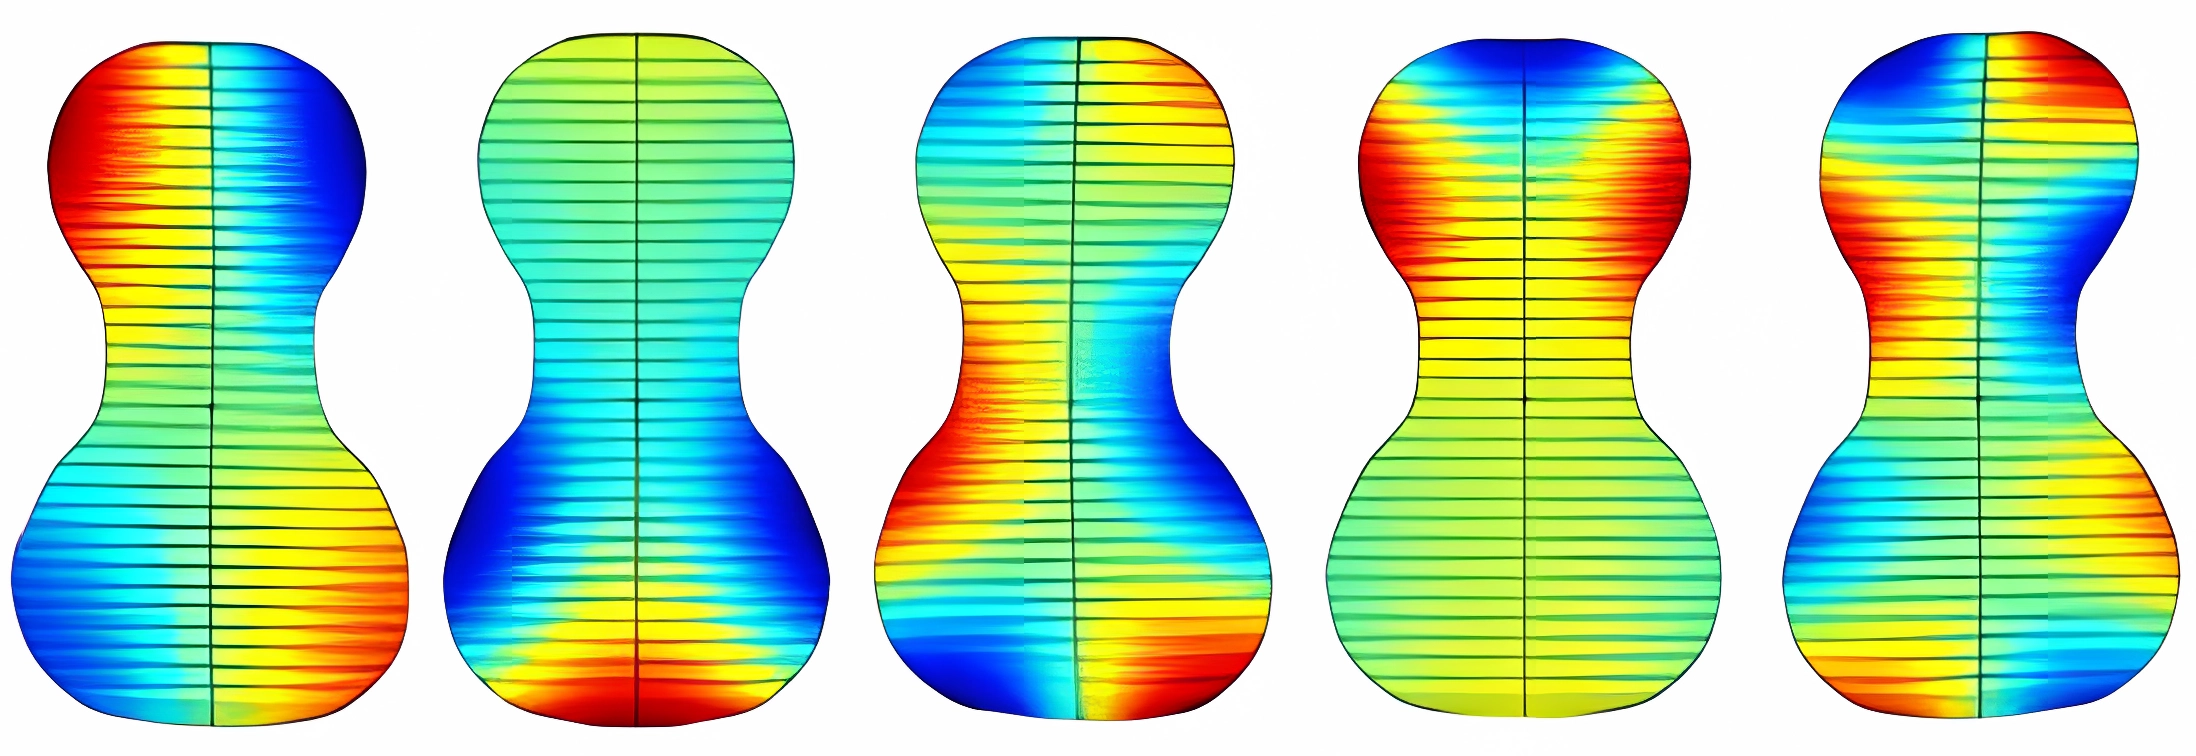
\includegraphics[width=1\linewidth]{CUMCMThesis-master/figures/gaoqing.png}\caption{振型高清图}
\label{fig}
\end{figure}

\subsubsection{最小二乘拟合方法概述}
为保证可读性,本节之中使用符号说明如表~\ref{table-7}~所示。
\begin{table}[H]
	\caption{\textbf{3.3.3节符号说明}}%title
	\centering
	\begin{tabular}{ll}% four columns
		\hline %begin the first line
		符号   &  含义  \\
		\hline %begin the second line
		$S\left(a_{ij}\right)$&所有观测点的误差平方和\\
		$a_{ij}^{(k)}$&第$k$次的参数迭代值\\
		$\gamma_1$&迭代学习率\\
		$J$&雅可比矩阵\\
		$r\left(a_{ij}\right)$&残差\\
		$\gamma_2$&调节优化方向和距离的参数\\
		\hline %begin the third line
	\end{tabular}\label{table-7}
\end{table}
在进行拟合前,先简要介绍最小二乘拟合的数学原理。非线性最小二乘拟合是一种用于处理非线性关系的模型方程拟合问题,它通过最小化预测与实际观测之间的误差平方和来对待估计参数求解。但由于模型本身的复杂性,往往不存在解析解。

以~\eqref{34}~为例,用已有的观测数据$\left(
x,y\right)$与假设方程$\varphi\left(x,y;a_{ij}\right)$定义目标函数$S\left(a_{ij}\right)$为所有观测点的误差平方和:
\begin{equation}
    S\left(a_{ij}\right)=\sum_{i=0}^n\sum_{j=0}^m\left[\varphi\left(x,y;a_{ij}\right)-\varphi\left(x,y\right)\right]^2,\label{36}
\end{equation}
由于$\varphi\left(x,y\right)$为非线性函数,其不一定存在解析解,需要使用数值迭代的方案对其求解,常用的三种数值迭代的方案将在下面解释。

梯度下降法是一种用迭代寻找函数的局部最小值。在非线性最小二乘问题中,其数学公式表达为:
\begin{equation}
    a_{ij}^{(k+1)}=\gamma_1 \bigtriangleup S\left(a_{ij}^k\right),\label{37}
\end{equation}
其中$a_{ij}^{(k)}$是第$k$次的参数迭代值,$\gamma_1$是迭代学习率。

高斯-牛顿法专门用于解决非线性最小二乘问题,基于泰勒展开将非线性问题局部线性化。其数学公式表达为:
\begin{equation}
    a_{ij}^{(k+1)}=a_{ij}^{(k)}-\left(J^TJ\right)^{-1}J^Tr\left(a_{ij}^{(k)}\right),\label{38}
\end{equation}
其中$J$是雅可比矩阵,$r\left(a_{ij}\right)$表示残差。

Levenberg-Marquardt算法是高斯-牛顿法的一个改进,增加了一个调整参数以改善收敛性。为优化雅可比矩阵$J$行列式为0,其逆不存在时的情况。其数学公式表达为:
\begin{equation}
    a_{ij}^{(k+1)}=a_{ij}^{(k)}-\left(J^TJ+\gamma_2 \textbf{diag}\left(J^TJ\right)^{-1}J^Tr\left(a_{ij}^{(k)}\right)\right), \label{39}
\end{equation}
其中$\gamma_2$作为调节优化方向和距离的参数。
\subsection{问题四:材料拟合}
针对于材料再拟合问题,在前一部分的问题分析中,已经提出~\eqref{25}\eqref{26}~两个微分方程,并在~\eqref{28}~给出~\eqref{25}~的解析解。若想进行材料拟合问题,即对微分方程做积分,转化为积分方程问题再进一步求解得到材料属性随位置变化的参数,为完成这一假设,引入材料变量$\phi$作为不同材料问题的假设,所以相较4.1,4.2,4.3节,修改后的全新符号说明如表~\ref{table-8}~所示。

\begin{table}[H]
	\caption{\textbf{3.4节符号说明}}%title
	\centering
	\begin{tabular}{ll}% four columns
		\hline %begin the first line
		符号   &  含义  \\
		\hline %begin the second line
		$\phi$&材料变量\\
  	$E(x,y;\phi)$&随材料变化的弹性模量\\
		$rho(x,y;\phi)$&随材料变化的密度\\
		$\nu(x,y;\phi)$&随材料变化的泊松比\\
        $h(x,y;\phi)$&随材料变化的厚度\\
		\hline %begin the third line
	\end{tabular}\label{table-8}
\end{table}
计算过程针对五个不同的模态,要找到$\phi$找到正确与之对应的数学参数,即本节的目标函数为:
\begin{equation}
    S\left(\phi\right)=\sum_{j=1}^5\int\int\left[\varphi_j\left(x_\alpha,x_\beta;\phi\right)-\varphi\left(x_\alpha,x_\beta\right)\right], \label{40}
\end{equation}
进一步对积分方程求数值解即可得到需要的材料参数,在前面部分建立完整的理论模型后,问题四本身并不复杂,但积分方程求数值解本身是无比困难的。
\section{模型求解}
\subsection{问题一:经典薄板结果汇报}
在计算过程中选取制作乐器的常用材料:云杉木材、铜、玻璃纤维复合材料与碳纤维作为研究材料,各材料参数如表~\ref{table1}~所示。

对经典薄板理论微分方程求解结果选择参考附件给出的五种频率来表现:(1)82HZ,(2)158HZ,(3)218HZ,(4)231HZ,(5)331HZ。并额外考虑范围(6)1500HZ。其振型分布如图\ref{fig_4}、图\ref{fig_5}、图\ref{fig_6}与图\ref{fig_7}所示。作为验证现使用弹性耦合法与瑞雷法计算模态振频作为补充,验证近似解算法的可靠性。结果如表~\ref{lizi}所示。

\begin{table}[htb]
\centering
\caption{问题一材料参数}
\label{table1}
\begin{tabular}{@{}ccccc@{}}
\toprule
\textbf{材料名称} & \textbf{切变模量/GPa} & \textbf{泊松比} & \textbf{密度/kg/m$^3$} & \textbf{杨氏模量/GPa} \\
\midrule
云杉木材 & 2-4 & 0.2-0.5 & 400-600 & 0.2-0.5 \\
铜 & 40-48 & 0.34 & 8900 & 110-130 \\
玻璃纤维复合材料 & 5-15 & 0.2-0.4 & 1600-2000 & 20-80 \\
碳纤维 & 100-150 & 0.2-0.3 & 1500-2000 & 200-700 \\
\bottomrule
\end{tabular}
\end{table}

\begin{table}[htb]
\centering
\caption{铜质均匀薄板的固有频率}
\label{table1}
\begin{tabular}{@{}ccccc@{}}
\toprule
\textbf{模态} & \textbf{弹性耦合法计算的固有频率} & \textbf{瑞雷法计算出的固有频率} & \textbf{Ansys计算出的固有频率}  \\
\midrule
(1,1) & 80.97 &104.62 & 81.22 \\
(1,2)& 95.52 & 113.26  & 96.31 \\
(1,3) & 126.62 & 134.63 & 122.47 \\
(2,1) & 174.99 & 212.92 & 170.23 \\
(2,2) & 182.17  & 219.91 & 183.14 \\
(2,3) & 200.24  & 236.23 & 200.63 \\
(3,1) & 308.89  & 359.76 & 309.27 \\
(3,2) & 313.02  & 366.11 & 314.26 \\
(3,3) & 323.02  & 380.09 & 324.39 \\
\bottomrule
\end{tabular}\label{lizi}
\end{table}
\begin{figure*}[htbp]
\centering
\subfloat[82HZ]{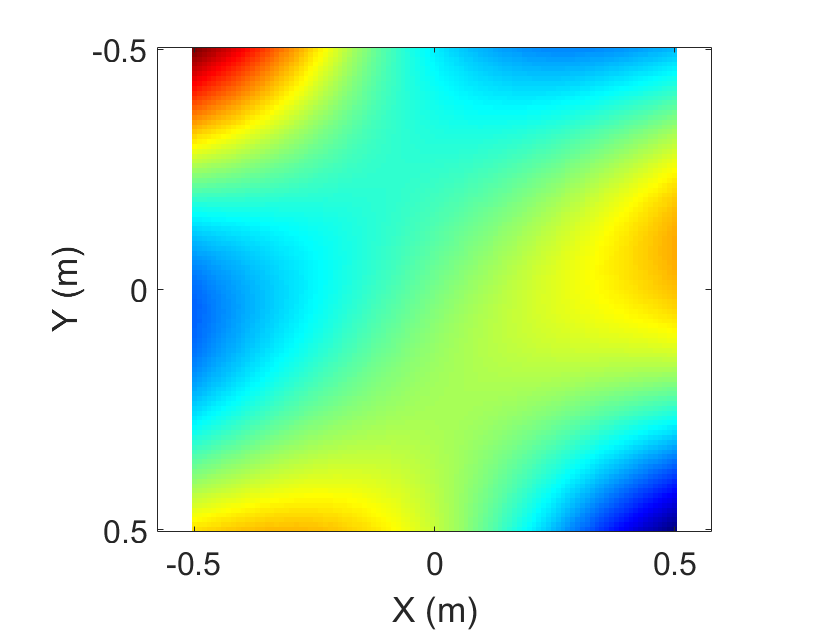
\includegraphics[width=2.05in]{CUMCMThesis-master/figures/1.1.png}%
\label{fig_first_case}}
\hfil
\subfloat[158HZ]{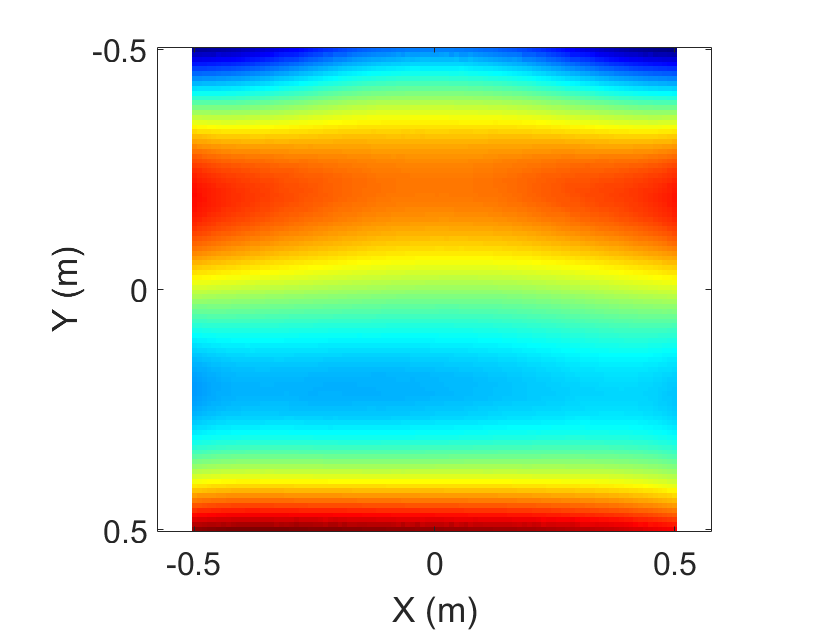
\includegraphics[width=2.05in]{CUMCMThesis-master/figures/1.2.png}%
\label{fig_second_case}}
\hfil
\subfloat[218HZ]{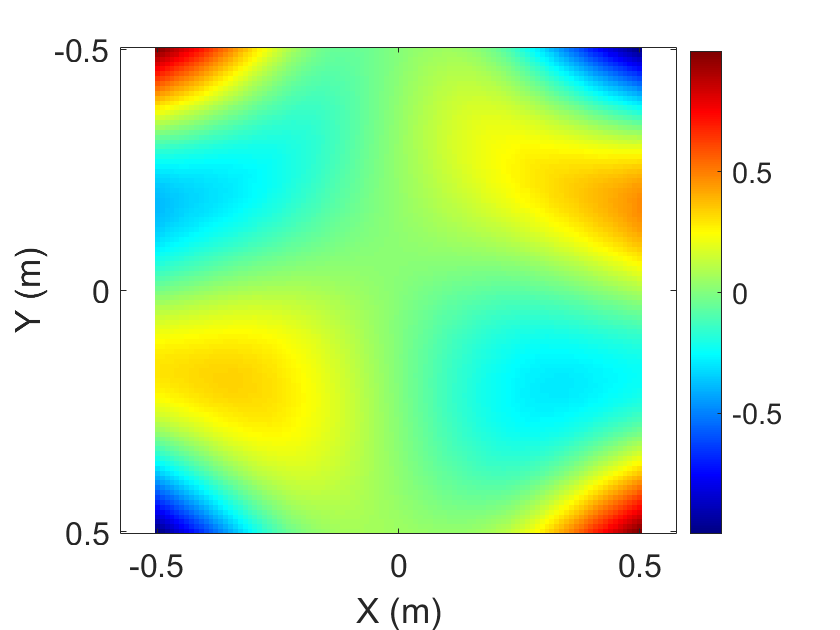
\includegraphics[width=2.05in]{CUMCMThesis-master/figures/1.3.png}%
\label{fig_first_case}}
\hfil
\subfloat[231HZ]{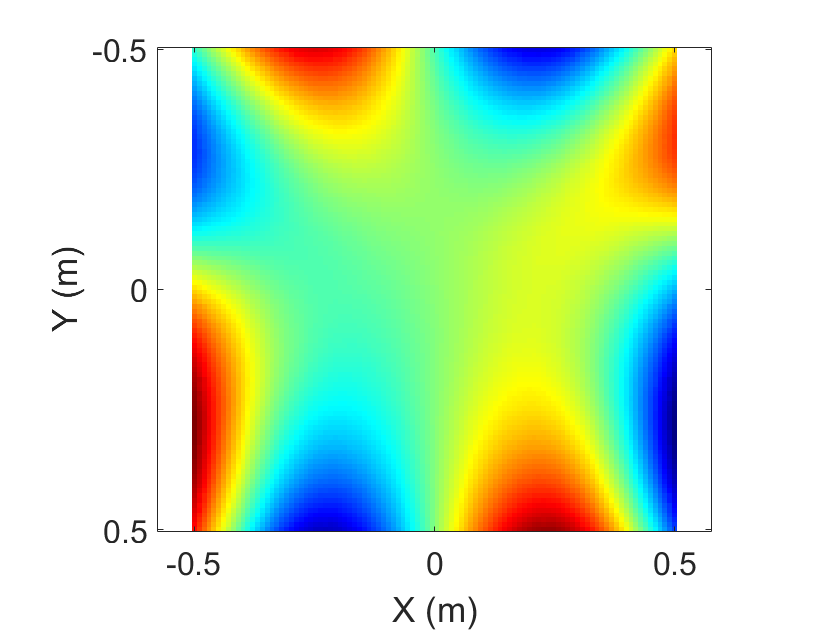
\includegraphics[width=2.05in]{CUMCMThesis-master/figures/1.4.png}%
\label{fig_first_case}}
\hfil
\subfloat[331HZ]{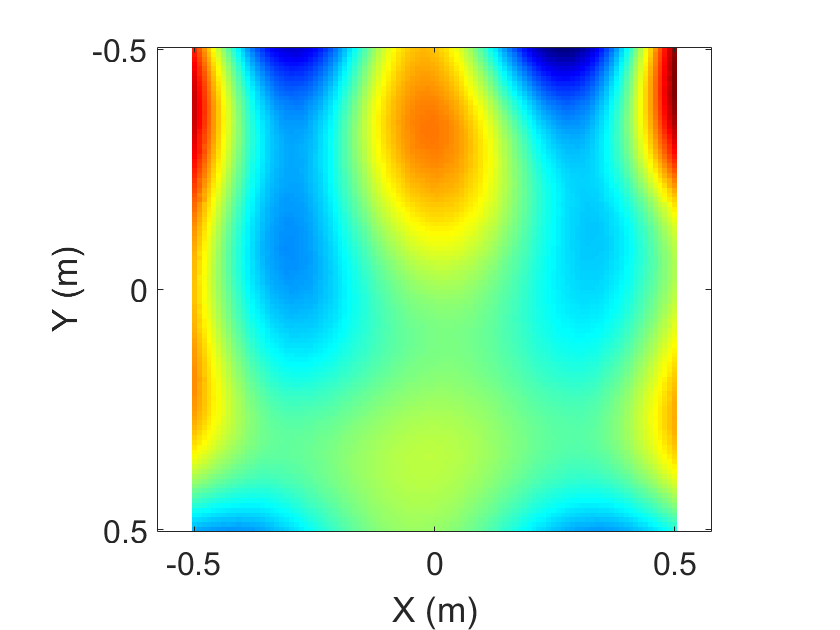
\includegraphics[width=2.05in]{CUMCMThesis-master/figures/1.5.png}%
\label{fig_first_case}}
\hfil
\subfloat[1500HZ]{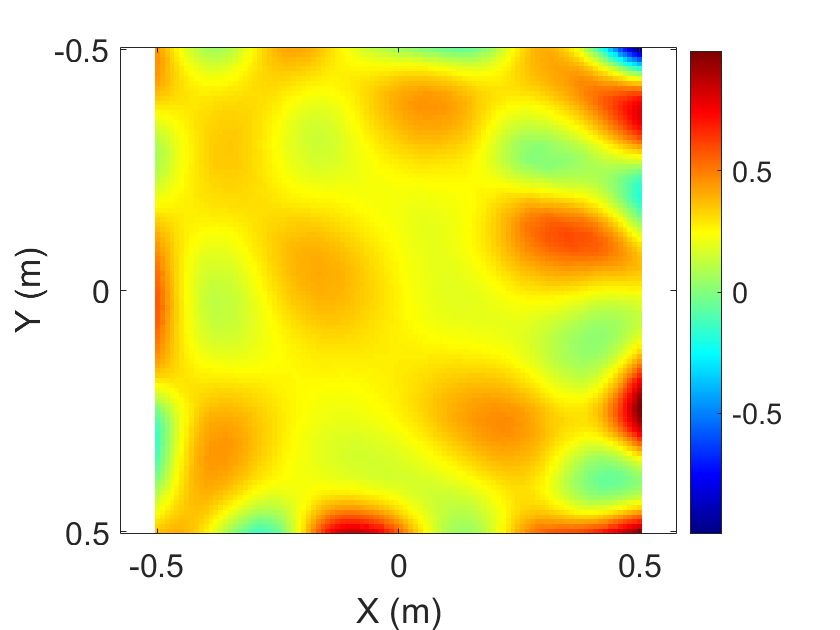
\includegraphics[width=2.05in]{CUMCMThesis-master/figures/1.6.png}%
\label{fig_first_case}}
\hfil
\caption{矩形云杉木薄板振型}
\label{fig_4}
\vspace{-0.4cm}
\end{figure*}

\begin{figure*}[!htbp]
\centering
\subfloat[82HZ]{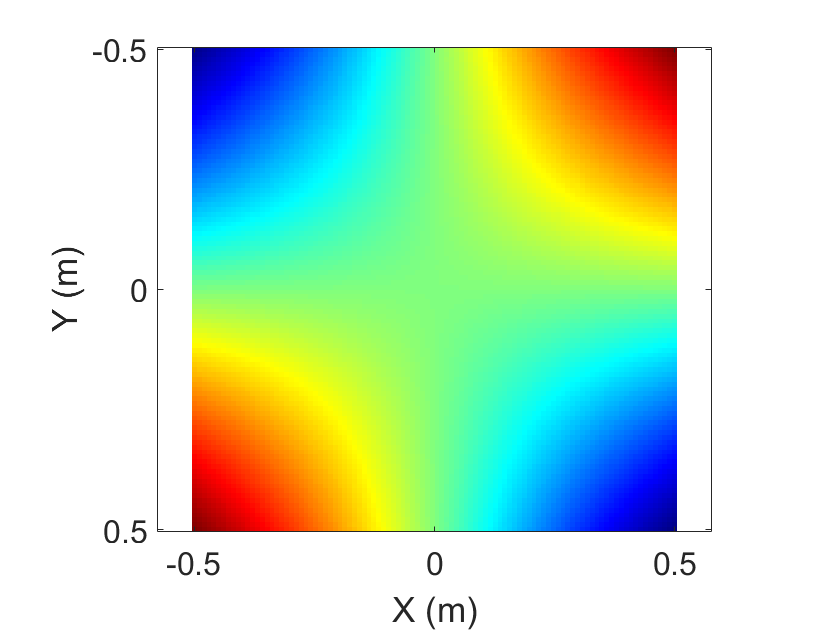
\includegraphics[width=2.05in]{CUMCMThesis-master/figures/2.1.png}%
\label{fig_first_case}}
\hfil
\subfloat[158HZ]{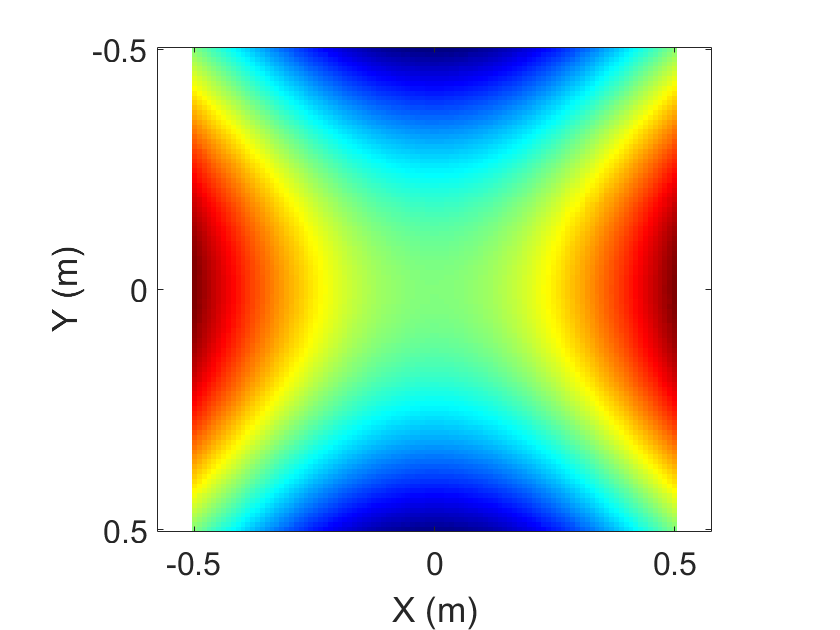
\includegraphics[width=2.05in]{CUMCMThesis-master/figures/2.2.png}%
\label{fig_second_case}}
\hfil
\subfloat[218HZ]{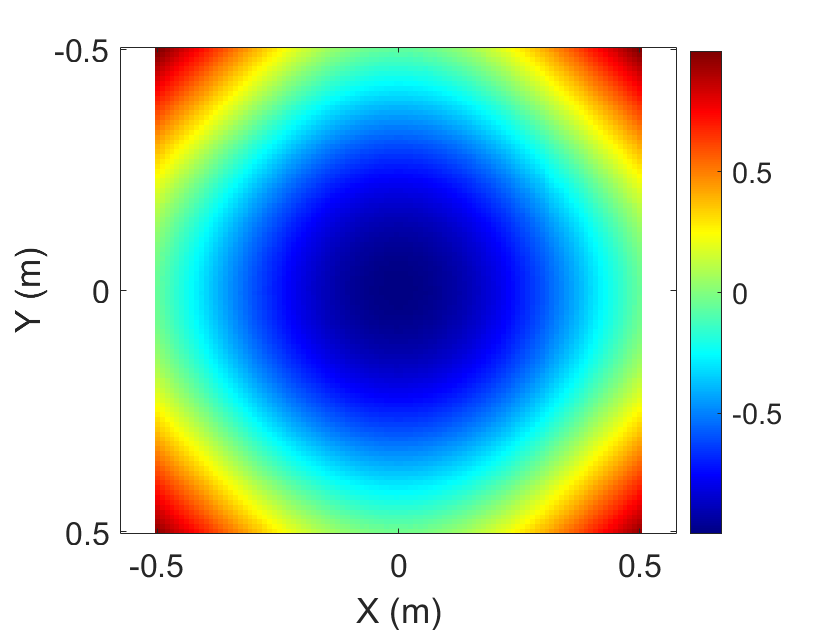
\includegraphics[width=2.05in]{CUMCMThesis-master/figures/2.3.png}%
\label{fig_first_case}}
\hfil
\subfloat[231HZ]{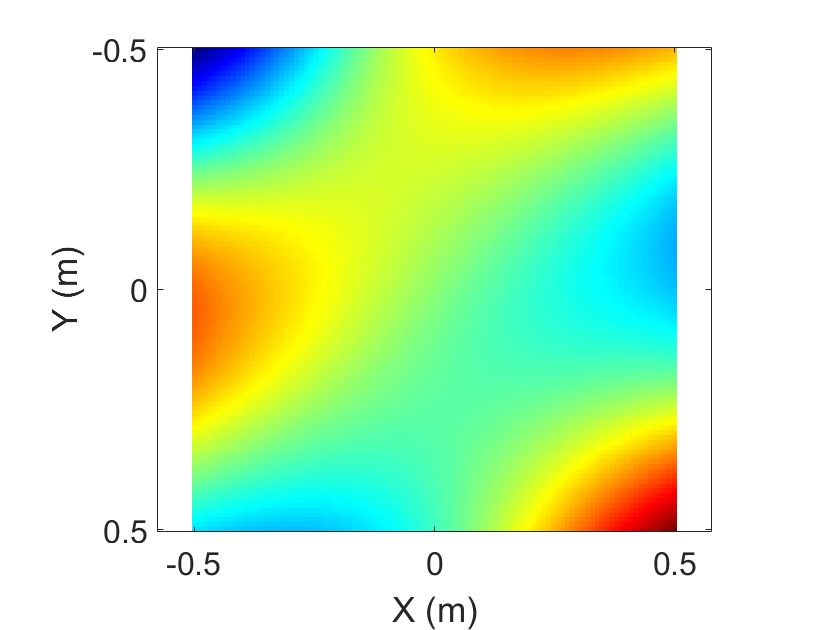
\includegraphics[width=2.05in]{CUMCMThesis-master/figures/2.4.png}%
\label{fig_first_case}}
\hfil
\subfloat[331HZ]{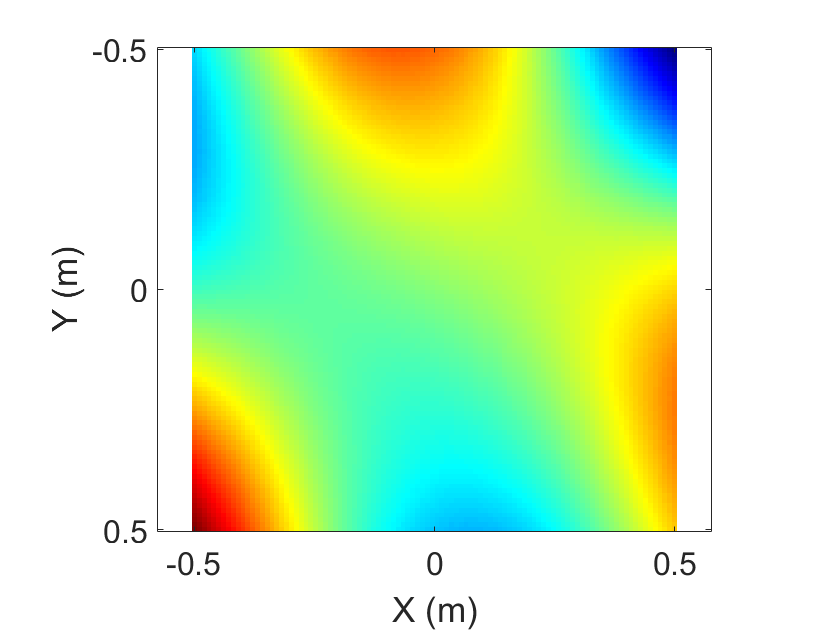
\includegraphics[width=2.05in]{CUMCMThesis-master/figures/2.5.png}%
\label{fig_first_case}}
\hfil
\subfloat[1500HZ]{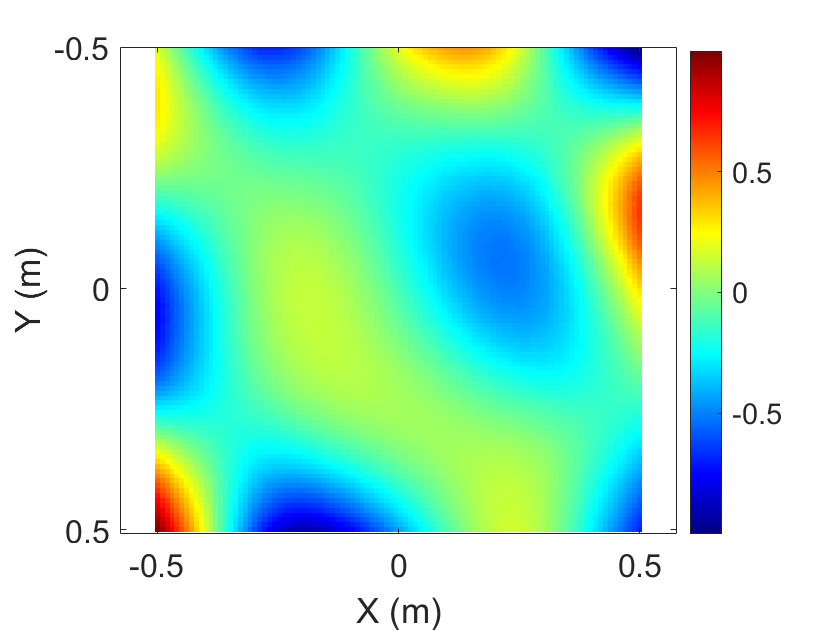
\includegraphics[width=2.05in]{CUMCMThesis-master/figures/2.6.png}%
\label{fig_first_case}}
\hfil
\caption{矩形铜薄板振型}
\label{fig_5}
\vspace{-0.4cm}
\end{figure*}
\begin{figure*}[htbp]
\centering
\subfloat[231HZ]{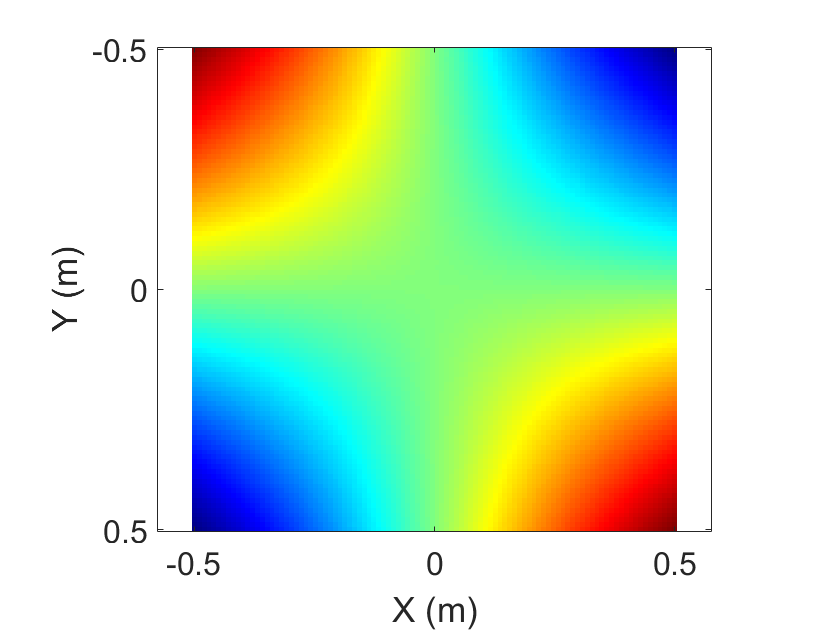
\includegraphics[width=2.05in]{CUMCMThesis-master/figures/3.1.png}%
\label{fig_first_case}}
\hfil
\subfloat[331HZ]{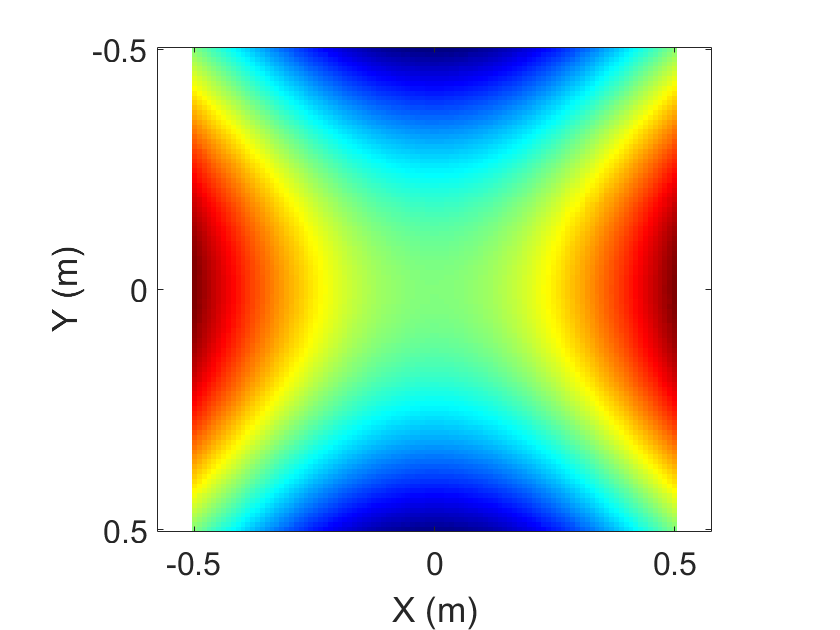
\includegraphics[width=2.05in]{CUMCMThesis-master/figures/3.2.png}%
\label{fig_first_case}}
\hfil
\subfloat[1500HZ]{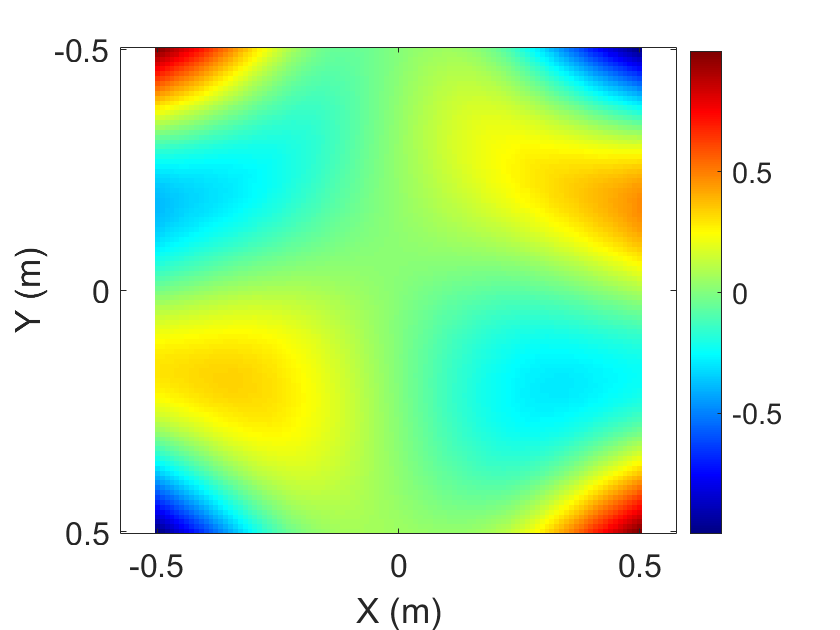
\includegraphics[width=2.05in]{CUMCMThesis-master/figures/3.3.png}%
\label{fig_first_case}}
\hfil
\caption{矩形玻璃纤维复合材料薄板振型(模拟过程之中发现231HZ以下薄板无自然震动形态)}
\label{fig_6}
\vspace{-0.4cm}
\end{figure*}

\begin{figure*}[htbp]
\centering
\subfloat[723HZ]{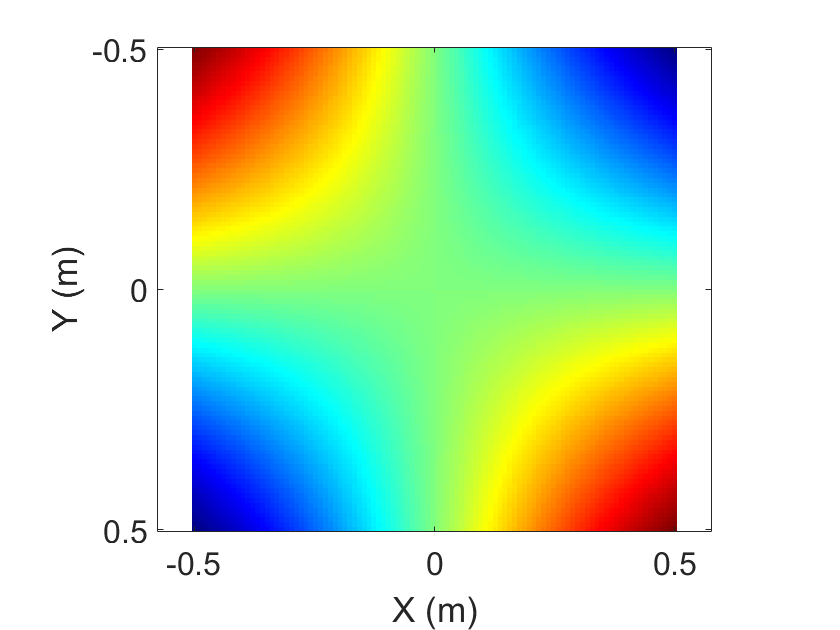
\includegraphics[width=2.05in]{CUMCMThesis-master/figures/4.1.png}%
\label{fig_first_case}}
\hfil
\subfloat[1053HZ]{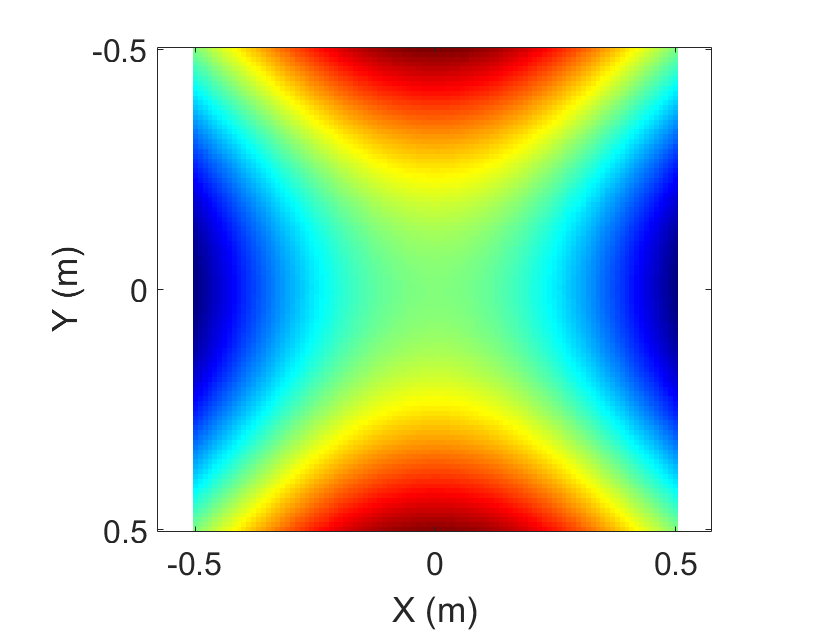
\includegraphics[width=2.05in]{CUMCMThesis-master/figures/4.2.png}%
\label{fig_first_case}}
\hfil
\subfloat[1176HZ]{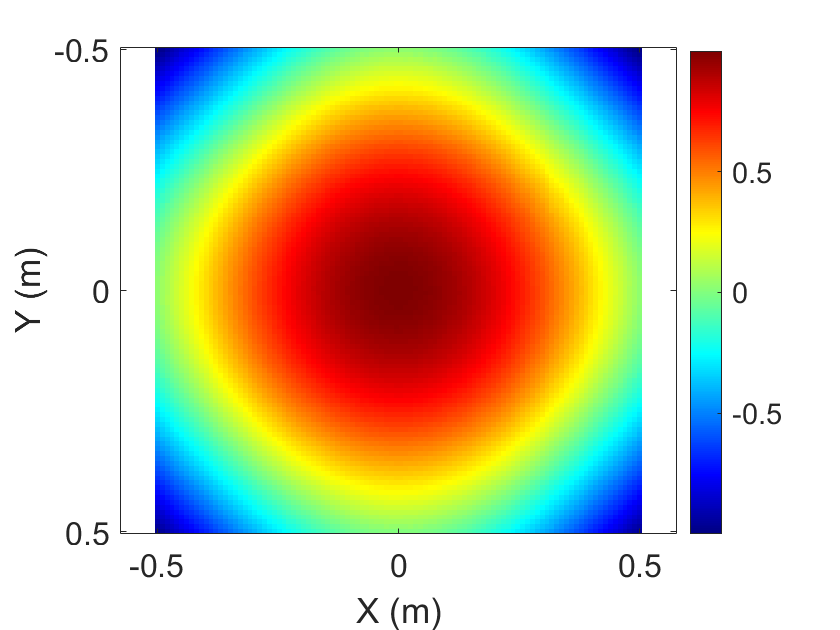
\includegraphics[width=2.05in]{CUMCMThesis-master/figures/4.3.png}%
\label{fig_first_case}}
\hfil
\caption{矩形碳纤维材料振型(模拟过程之中没有得到所需HZ下的振型,2000HZ下仅有这三种振型)}
\label{fig_7}
\vspace{-0.4cm}
\end{figure*}



\subsection{问题二:木材的各向异性}
木材作为非均质各向异性材料,较普通金属有着更好的性能,在公式~$(48)$中提到,如果一个各向异性材料具有横向同性,则它会退化至各向同性的材料方程,但木材的生长结构避免了这一点。这是优于数目由于生长方向的不同产生了其材质上的各向异性,简单的说,树木生长包括内两个方面:一是胸径增容大,二是高度增加,二者一为轴向,一为径向,故而形成了木材纵向并列的生长纹路,这种生长纹路进一步影响了木材受力时的变形程度。这导致普通的木材不会出现横向同性的情况,让音板的振动变得更为复杂,音色更为宽广。
\begin{figure}
    \centering
    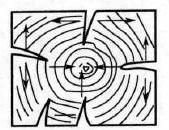
\includegraphics[width=0.5\linewidth]{CUMCMThesis-master/figures/mucai.jpg}
    \caption{木材的横向异性}
    \label{fig:enter-label}
\end{figure}
\subsection{问题二:参数方程仿真吉他振动板与复杂动力方程求解}
为制作薄音板,需提取附件中木材轮廓数据,在这一部分中选择对轮廓提取离散点的形式来得到吉他的轮廓示意图,提取得到的结果如图\ref{fig-8}所示。


对音板厚度进行拟合,这里采取对轮廓线求得坐标的方式进行拟合,这一步需要根据轮廓的坐标计算厚度的分布函数:
\begin{equation}
h\left(x_\alpha,x_\beta\right)=5-3\left(\frac{y}{20}\right)^2.
\end{equation}

拟合得到的结果如图\ref{fig-9}所示。在得到厚度分布函数后,可以将其带入~\eqref{21}~中得到其他材质函数的母函数~\cite{ref7}\cite{ref8}。试图对其进行求解。
\newpage
\begin{figure}[htbp]
\centering %图片居中
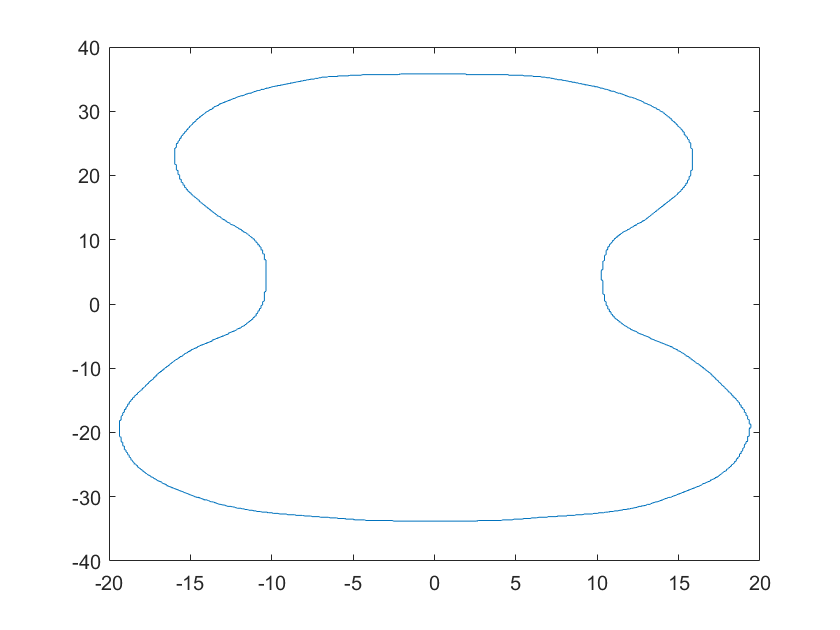
\includegraphics[width=0.45\linewidth]{CUMCMThesis-master/figures/Shape.png}\caption{音板轮廓线提取示意图}
\label{fig-8}
\end{figure}
\begin{figure}[htbp]
\centering %图片居中
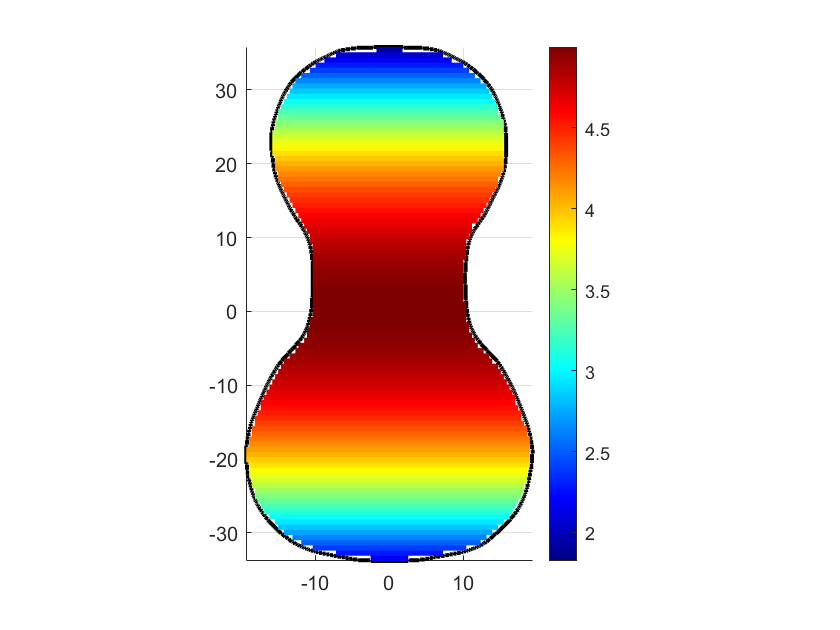
\includegraphics[width=0.8\linewidth]{CUMCMThesis-master/figures/hou.png}\caption{音板厚度拟合示意图}
\label{fig-9}
\end{figure}

但事实上,这一求解过程十分复杂,与前一部分的正方形均匀薄板不同,对不规则的非均匀薄板而言,从构造有限元到后续计算的过程均十分复杂。对问题一的求解时,采用~Partial Differential Equation Toolbox~这一成熟的~Matlab~分析工具箱协助进行分析。遗憾的是,这一工具箱并没有针对不同性质单元的有限元问题的调用接口。为解决问题,在后续的内容之中将详细介绍分别通过~Matlab~和~Python~两种语言实现的仿真结果,并深入分析其内部存在的问题与改良方式。

\subsubsection{Delaunay~三角剖分算法}
针对于不规则的闭合曲线,调用现有的网格分割函数构造单元是一种经典得到方法。但这一过程直接集成有限元赋值问题,导致实验过程之中不能直接导入有限元的厚度性质。我们在实验过程之中重构了原始函数,并使用~Delaunay~三角剖分避免生成细长的三角形,尽量使得三角形的最小角最大化,这避免细长单元对有限元分析的影响,并带来许多十分有利的性质:
\begin{itemize}
    \item \textbf{最大化最小角:}Delaunay~三角剖分避免生成细长的三角形,尽量使得三角形的最小角最大化,这对许多应用场景(如有限元分析)有好处。
    \item \textbf{凸包包含性:}Delaunay~三角剖分的外边界是这些点的凸包。
    \item \textbf{唯一性:}对于一组给定的点,如果这些点没有四点共圆的情况,则 Delaunay~三角剖分是唯一的。
\end{itemize}

现提供Delaunay~三角剖分算法的流程图如图~\ref{Dfigure}~所示。
\begin{figure}[H]
\centering %图片居中
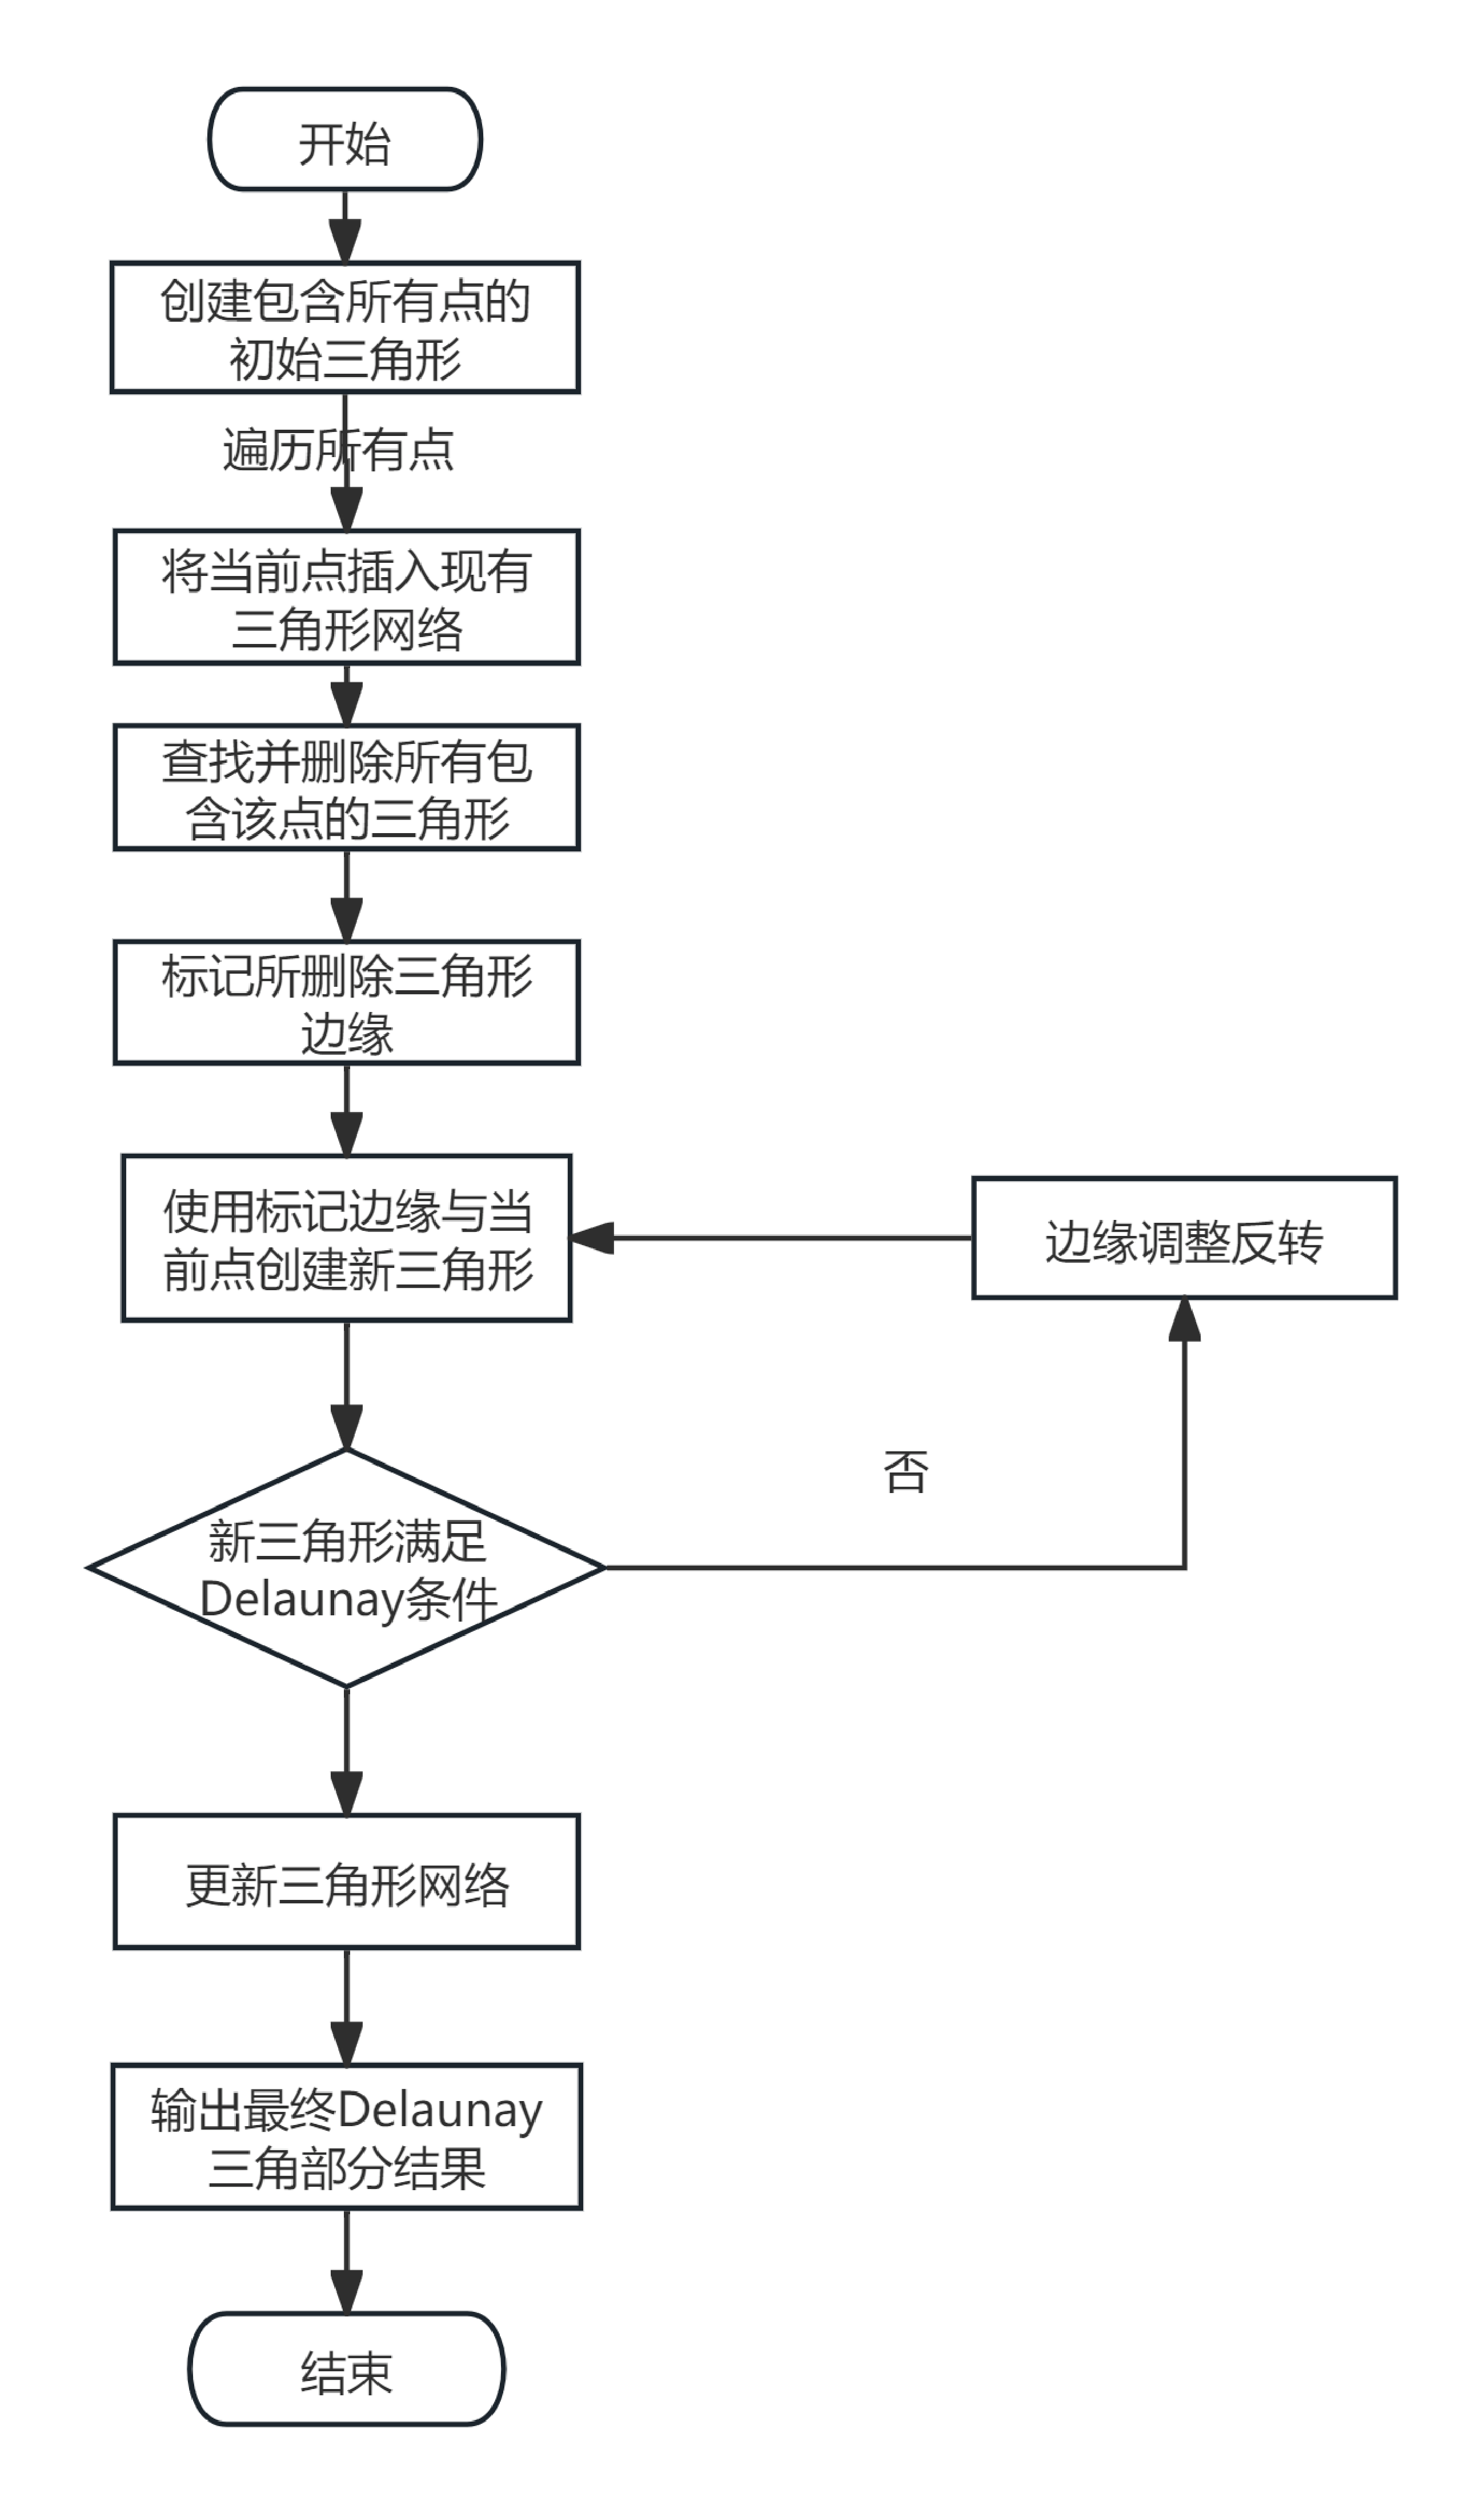
\includegraphics[width=0.5\linewidth,height=0.75\linewidth]{CUMCMThesis-master/figures/Dfigure.pdf}\caption{82HZ非均匀吉他形音板振动示意图}
\label{Dfigure}
\end{figure}
在得到剖分后的单位元网格后,可以进行有限元分析,但正如前文所说,这里并不能直接使用~Partial Differential Equation Toolbox~进行有限元分析,也需要构建全新的有限元仿真系统来解决问题。
\subsubsection{非均匀薄板有限元算法求解}
在均匀薄板的前提下,薄板的数值解可以调用有限元分析法API直接求解,但问题二是讨论非均匀薄板的有限元分析,所以根据需求设置全新的算法。刚度矩阵$K$可通过~\eqref{10}~\eqref{11}~进行设置,而质量矩阵$M$需要根据单位元节点的坐标与Jacobian矩阵的逆进行计算。对于四节点四边形单元,可以使用自然坐标$(\xi ,\eta)$进行插值。

	四节点四边形单元的形状函数$N$和其导数可以表示为:
	\begin{equation}
		N_i(\xi,\eta)=\frac{1}{4}(1+\xi \xi_i)(1+\eta \eta_i)\label{c1}
	\end{equation}
	其中,节点$i$的自然坐标$(\xi_i,\eta_i)$取值为$(\pm1,\pm1)$。
	
	形状函数对$\xi$和$\eta$的导数分别为:
	\begin{equation}
		\begin{aligned} 
		&\frac{\partial N_i}{\partial \xi}=\frac{1}{4}\eta_i(1+\eta \eta_i)\\
		&\frac{\partial N_i}{\partial \eta}=\frac{1}{4}\xi_i(1+\xi \xi_i)\\
	\end{aligned}\label{c2}
	\end{equation}
		
	Jacobian矩阵用于将自然坐标系下的导数转换为物理坐标系下的导数。将~\eqref{c2}~带入Jacobian矩阵,并通过求解Jacobian矩阵的逆得到$M$矩阵:
		\begin{equation}
		B=J^{-1}\begin{bmatrix}
			\frac{\partial N_i}{\partial \xi}&0\\
			0&\frac{\partial N_i}{\partial \eta}\\
			\frac{\partial N_i}{\partial \eta}&\frac{\partial N_i}{\partial \eta}\\
		\end{bmatrix}\label{c3}
	\end{equation}

至此,求出不同HZ下吉他形音板的振型状态,并将部分结果整理如图~\ref{guitarbufen}~所示,其完整版本见附录~\ref{fuluA}。 
\begin{figure}[H]
\centering %图片居中
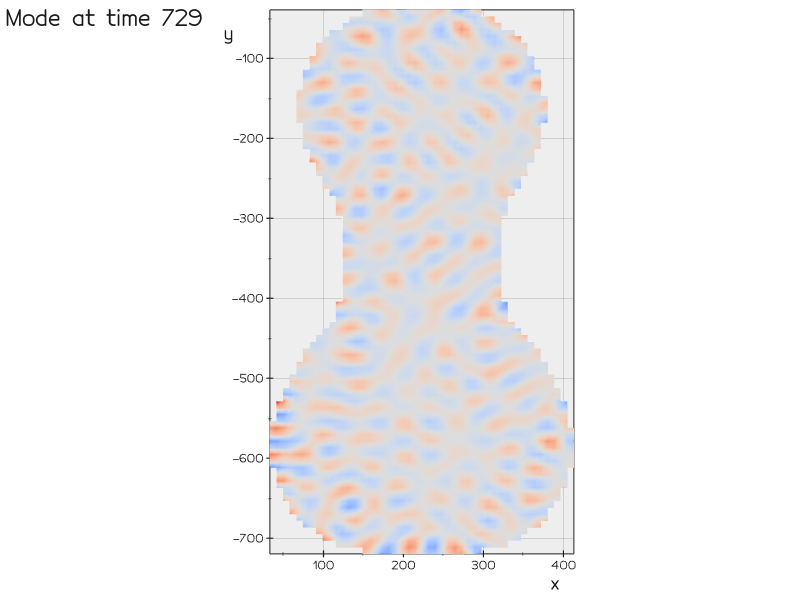
\includegraphics[width=0.7\linewidth]{CUMCMThesis-master/figures/82.png}\caption{82HZ非均匀吉他形音板振动示意图}
\label{guitarbufen}
\end{figure}
\subsection{问题三:振型函数拟合}
在拟合振型函数前,需提取振型高清图之中的振型信息,这里按照~\eqref{29}~\eqref{30}~的方案将五张图片的振型高清图之中的振型信息全部提取出来,其中部分信息如图~\ref{fig10},完整版见附录~\ref{fuluB}。
\begin{figure*}[htbp]
\centering
\subfloat[振型信息提取82HZ]{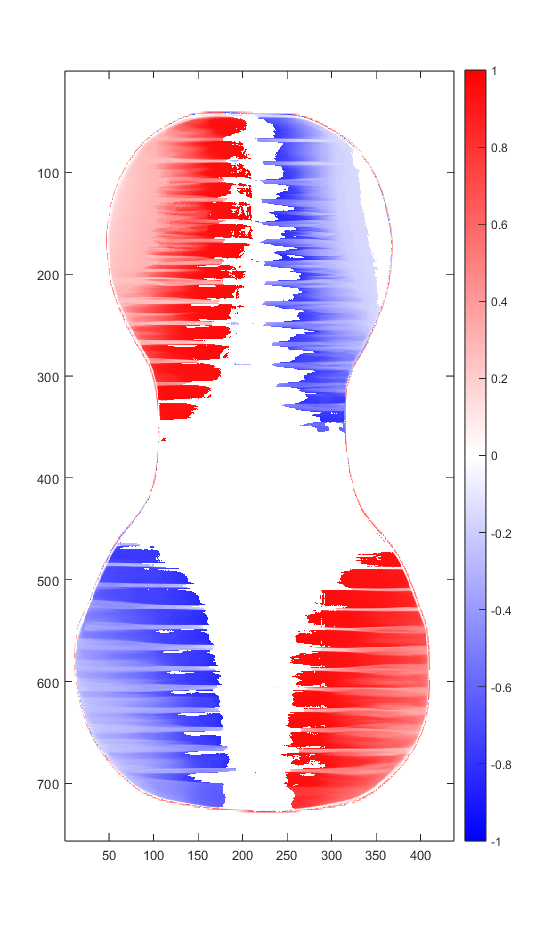
\includegraphics[width=2.5in]{CUMCMThesis-master/figures/4.3.1.png}%
\label{fig_first_case}}
\hfil
\subfloat[振兴信息提取331HZ]{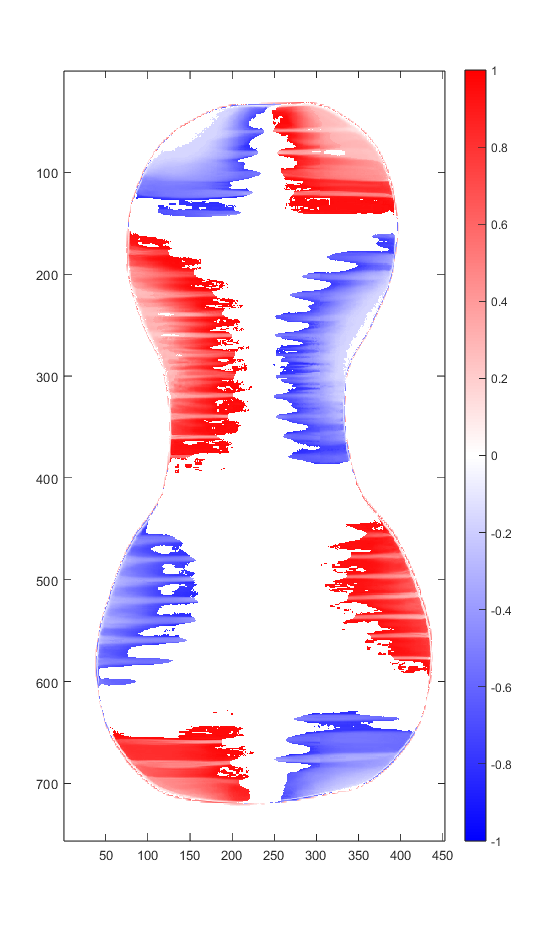
\includegraphics[width=2.5in]{CUMCMThesis-master/figures/4.3.5.png}%
\label{fig_first_case}}
\hfil
\caption{部分振型信息提取(完整版见附录~\ref{fuluB})}
\label{fig_4.3.1}
\vspace{-0.4cm}
\label{fig10}
\end{figure*}
而式~\eqref{34}~\eqref{35}~即为本节之中要拟合的函数,为表达清晰在此处再一次表述:
\begin{equation}
    \begin{aligned}
     \varphi\left(x,y\right)&=\sum_{i=0}^n\sum_{j=0}^ma_{ij}x^iy^j\\
\varphi\left(r,\theta\right)&=\sum_{n=0}^N A_n \cos\left(n\theta\right)J_n\left(\xi r\right)+B_n\sin\left(n\theta\right)J_n\left(\xi r\right).   \notag
    \end{aligned}
\end{equation}

使用最小二乘对两类振型函数分别进行拟合,不同振型函数对应的拟合误差如图~\ref{82wucha},完整版见附录~\ref{fuluC}。
\begin{figure*}[htbp]
\centering
\subfloat[82HZ振型拟合误差图]{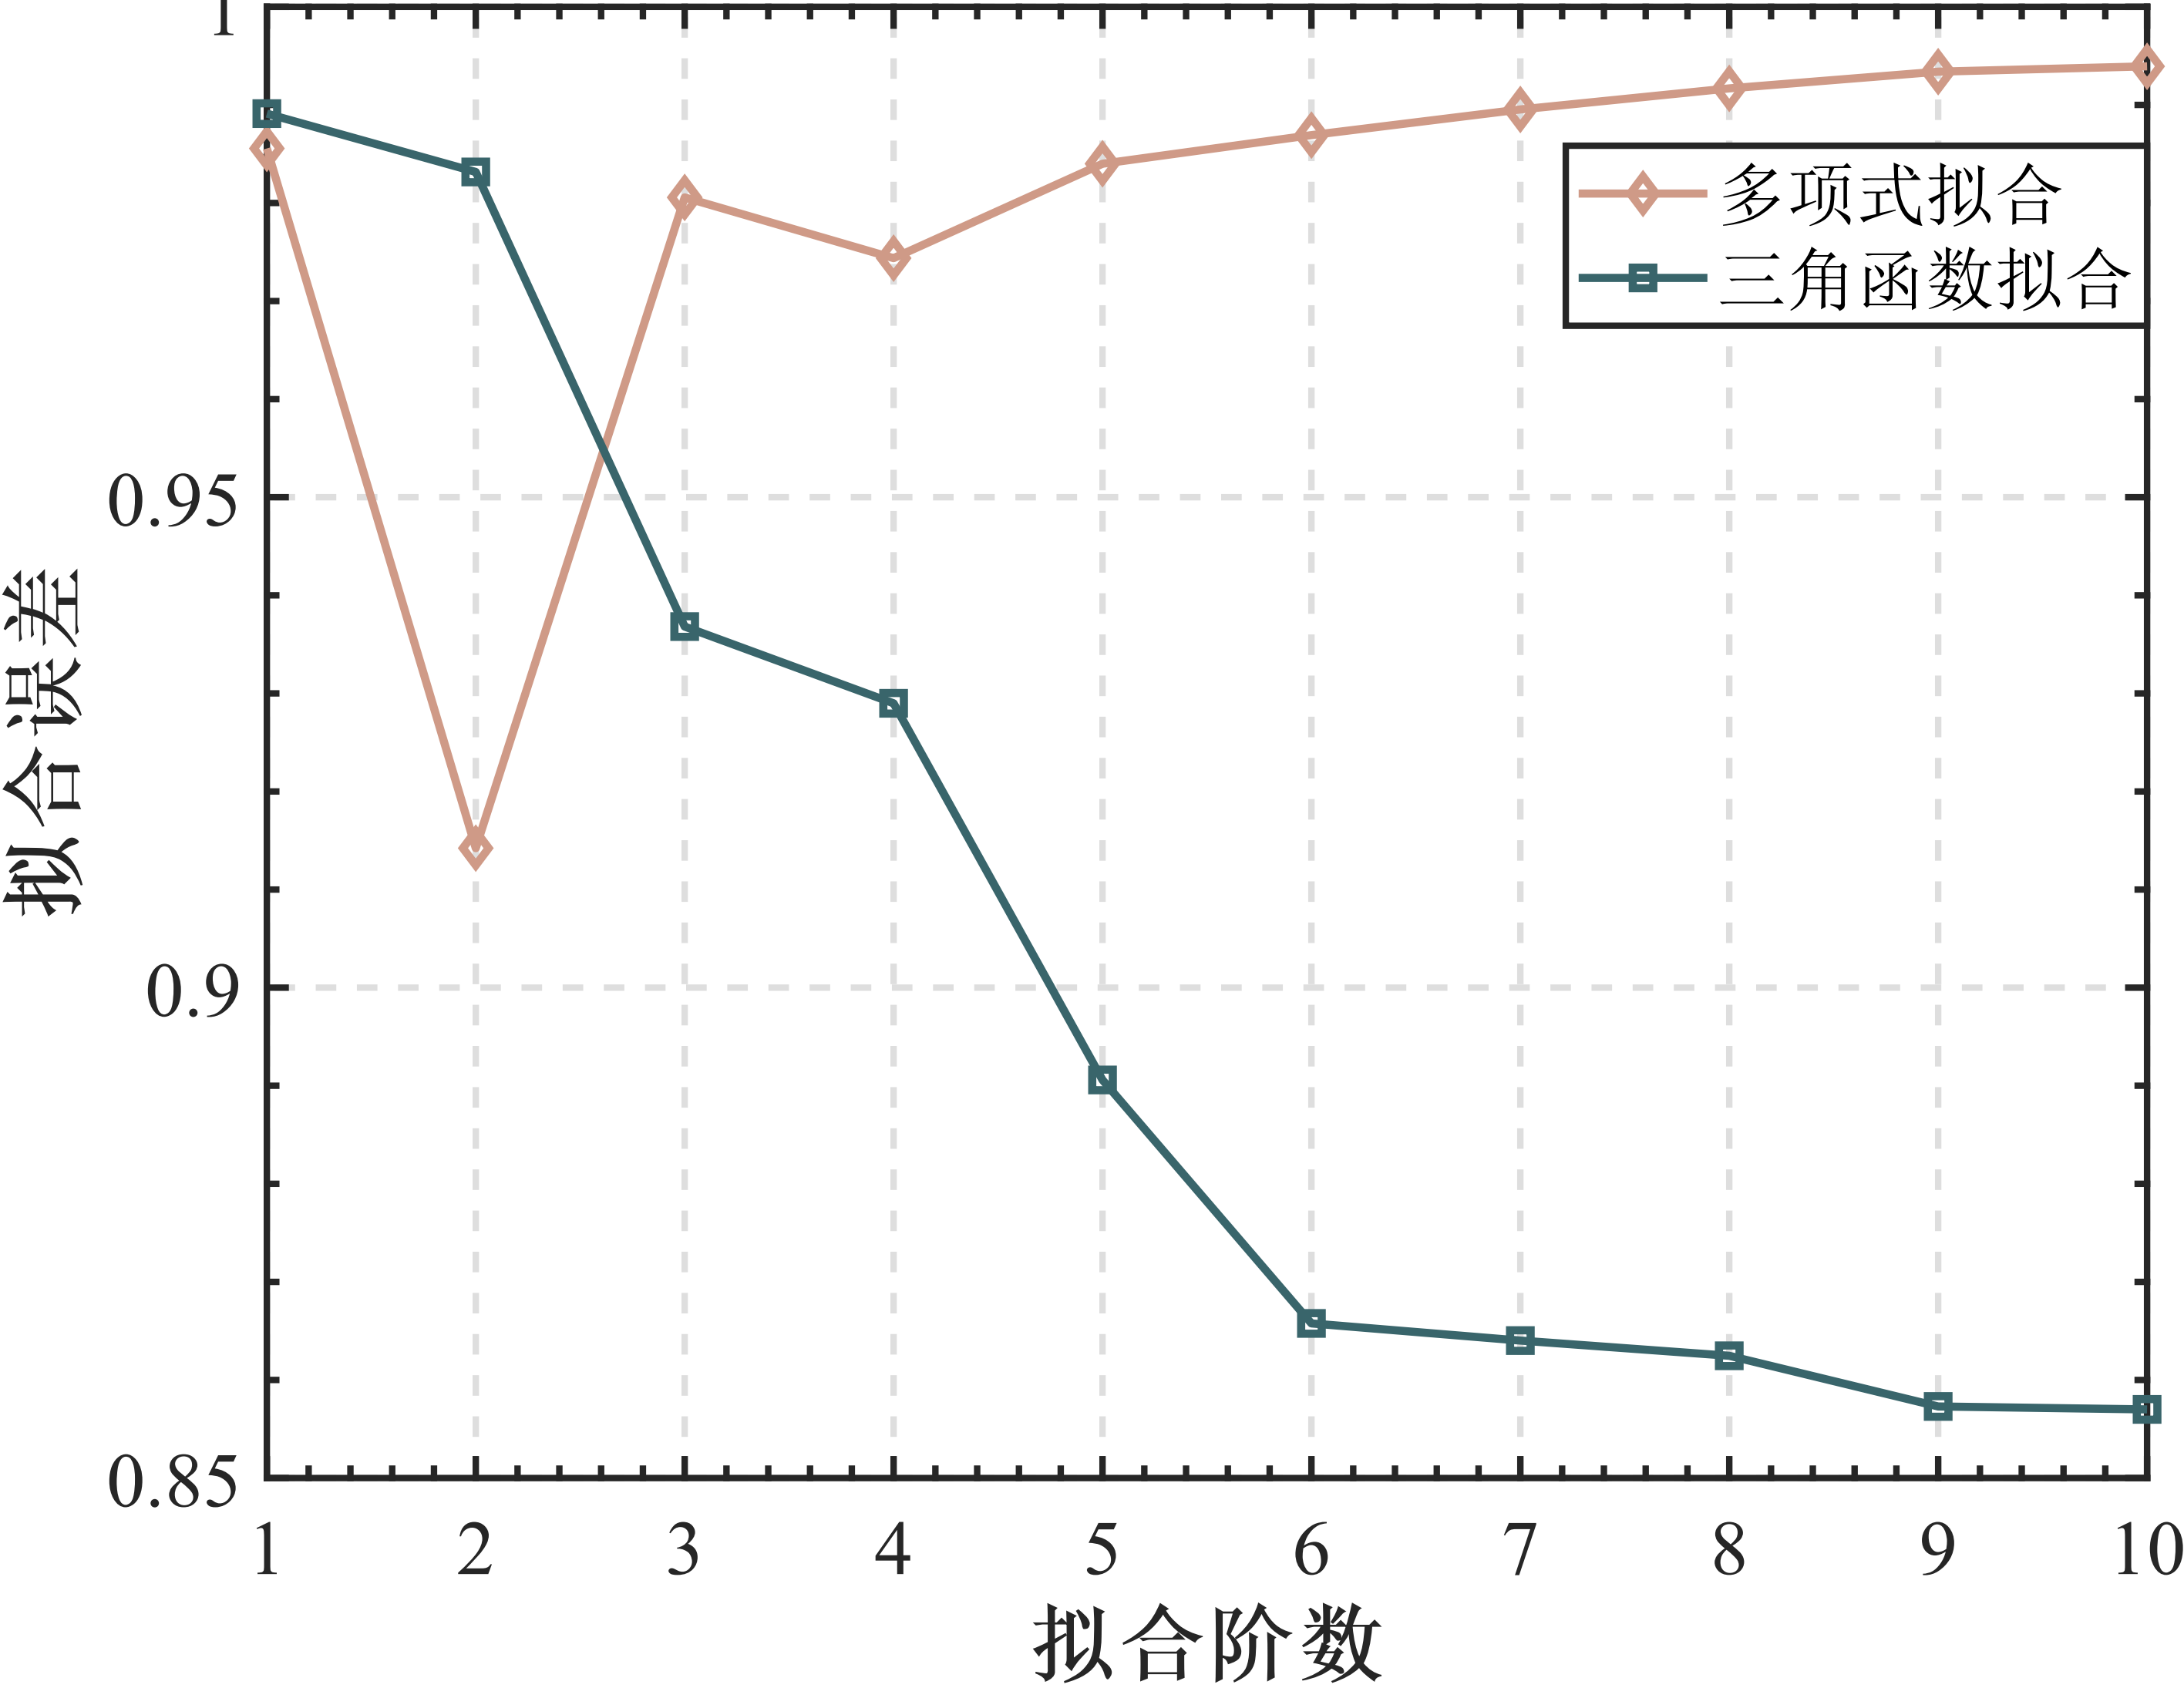
\includegraphics[width=3.1in]{CUMCMThesis-master/figures/1_00.png}%
\label{fig_first_case}}
\hfil
\subfloat[158HZ振型拟合误差图]{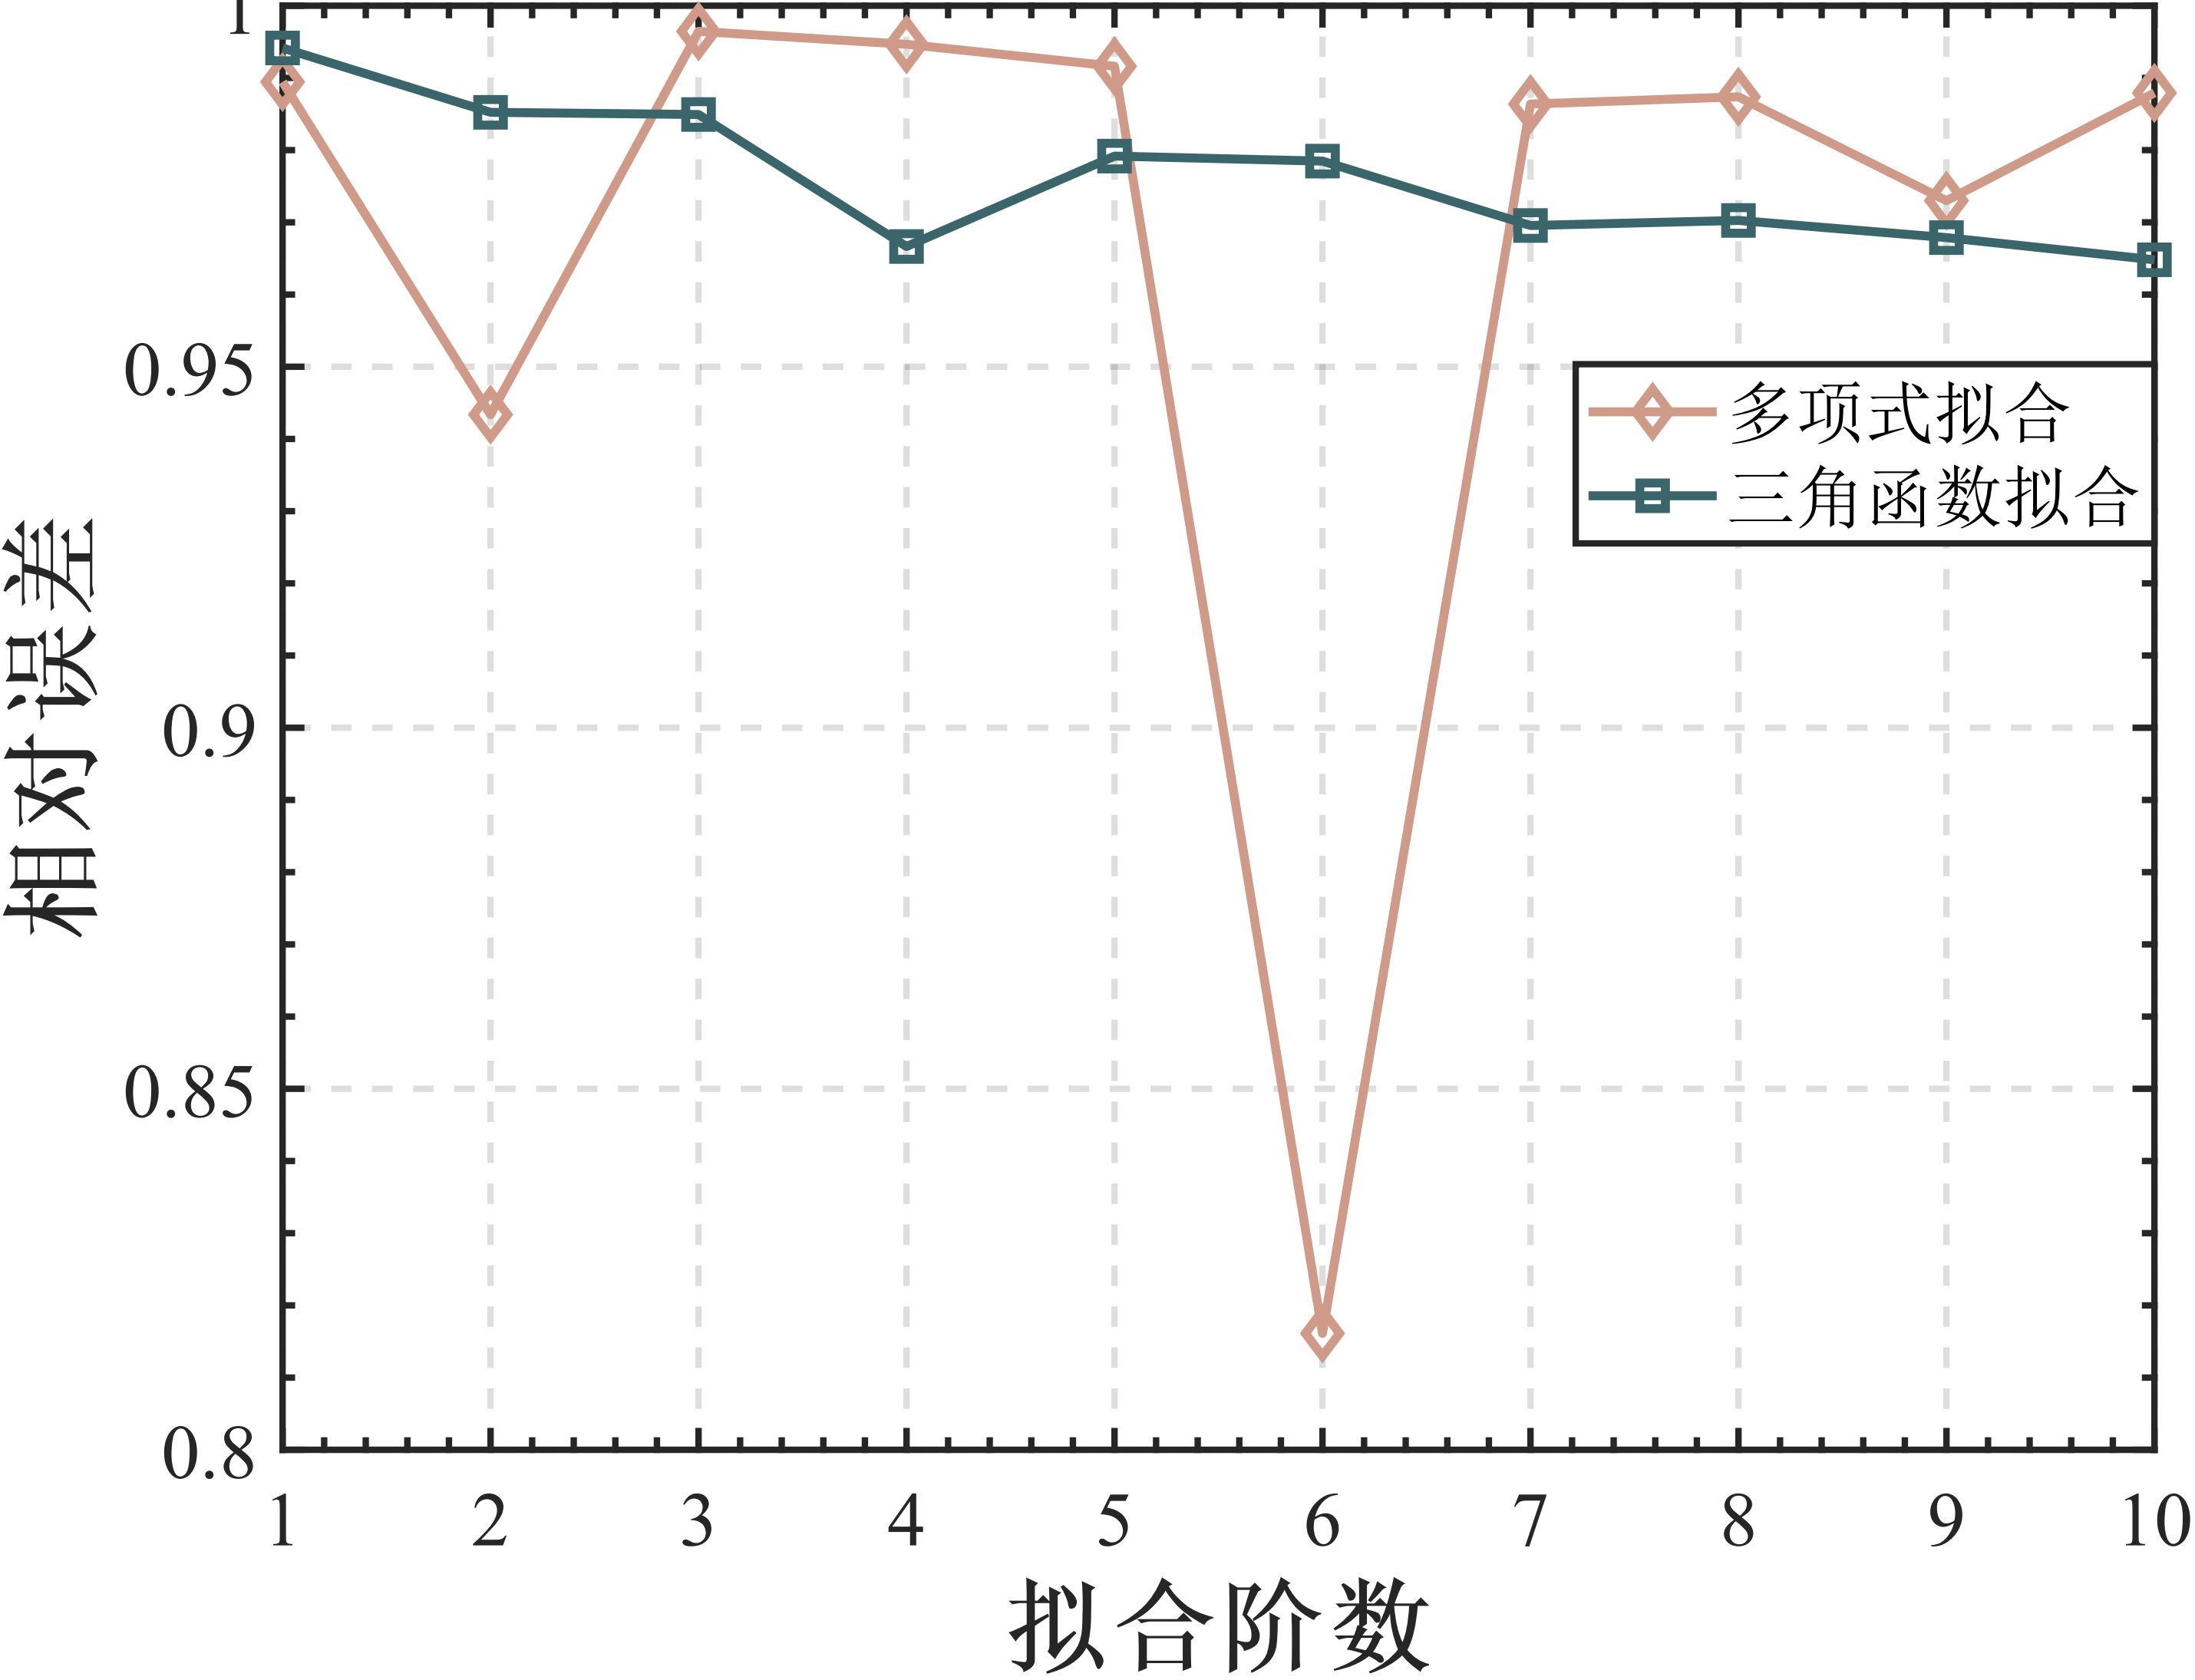
\includegraphics[width=3.1in]{CUMCMThesis-master/figures/2_00.png}%
\label{182}}
\hfil
\caption{部分振型拟合误差图(完整版见附录~\ref{fuluC})}
\label{fig_4.3.1}
\vspace{-0.4cm} \label{82wucha}
\end{figure*}

可以看到,多项式振型函数在拟合的过程之中出现拟合误差震荡的现象,这说明多项式振型函数不能很好的解释本次遇到的振型问题;而三角函数在拟合后收敛至确定值,其中的误差是图片读取时带来的误差,说明三角函数能很好的拟合振型函数。但值得怀疑的是,例如图~\ref{82wucha}~中的~\ref{182}~有多项式的震荡跌落点在三角拟合误差之下,这一内容将在5.2节之中进一步讨论。

为防止优化过程过拟合,在选择三角函数振型函数阶数时,只需选择梯度较陡部分的近似收敛点即可,其结果可从拟合误差图之中观测得到,最终不同HZ的振型重建阶数如表~\ref{table-HZ}~所示。
\begin{table}[H]
	\caption{\textbf{不同HZ下振型函数的选择}}%title
	\centering
	\begin{tabular}{ll}% four columns
		\hline %begin the first line
		不同的振动HZ   &  振型函数的形式  \\
		\hline %begin the second line
		82HZ&6阶三角和式\\
  	158HZ&4阶三角和式\\
		218HZ&6阶三角和式\\
		231HZ&4阶三角和式\\
        331HZ&9阶三角和式\\
		\hline %begin the third line
	\end{tabular}\label{table-HZ}
\end{table}
\subsection{问题四:材料拟合}
在实际求解的过程之中,遇到了积分方程拟合的雅可比矩阵为奇异矩阵的情况,哪怕引入微小扰动也没有妥善的解决这一难题。在数学求解受挫的情况下,我们采用另外一种方式:网格搜索材料参数,再对齐模态振型。
\begin{figure}
    \centering
    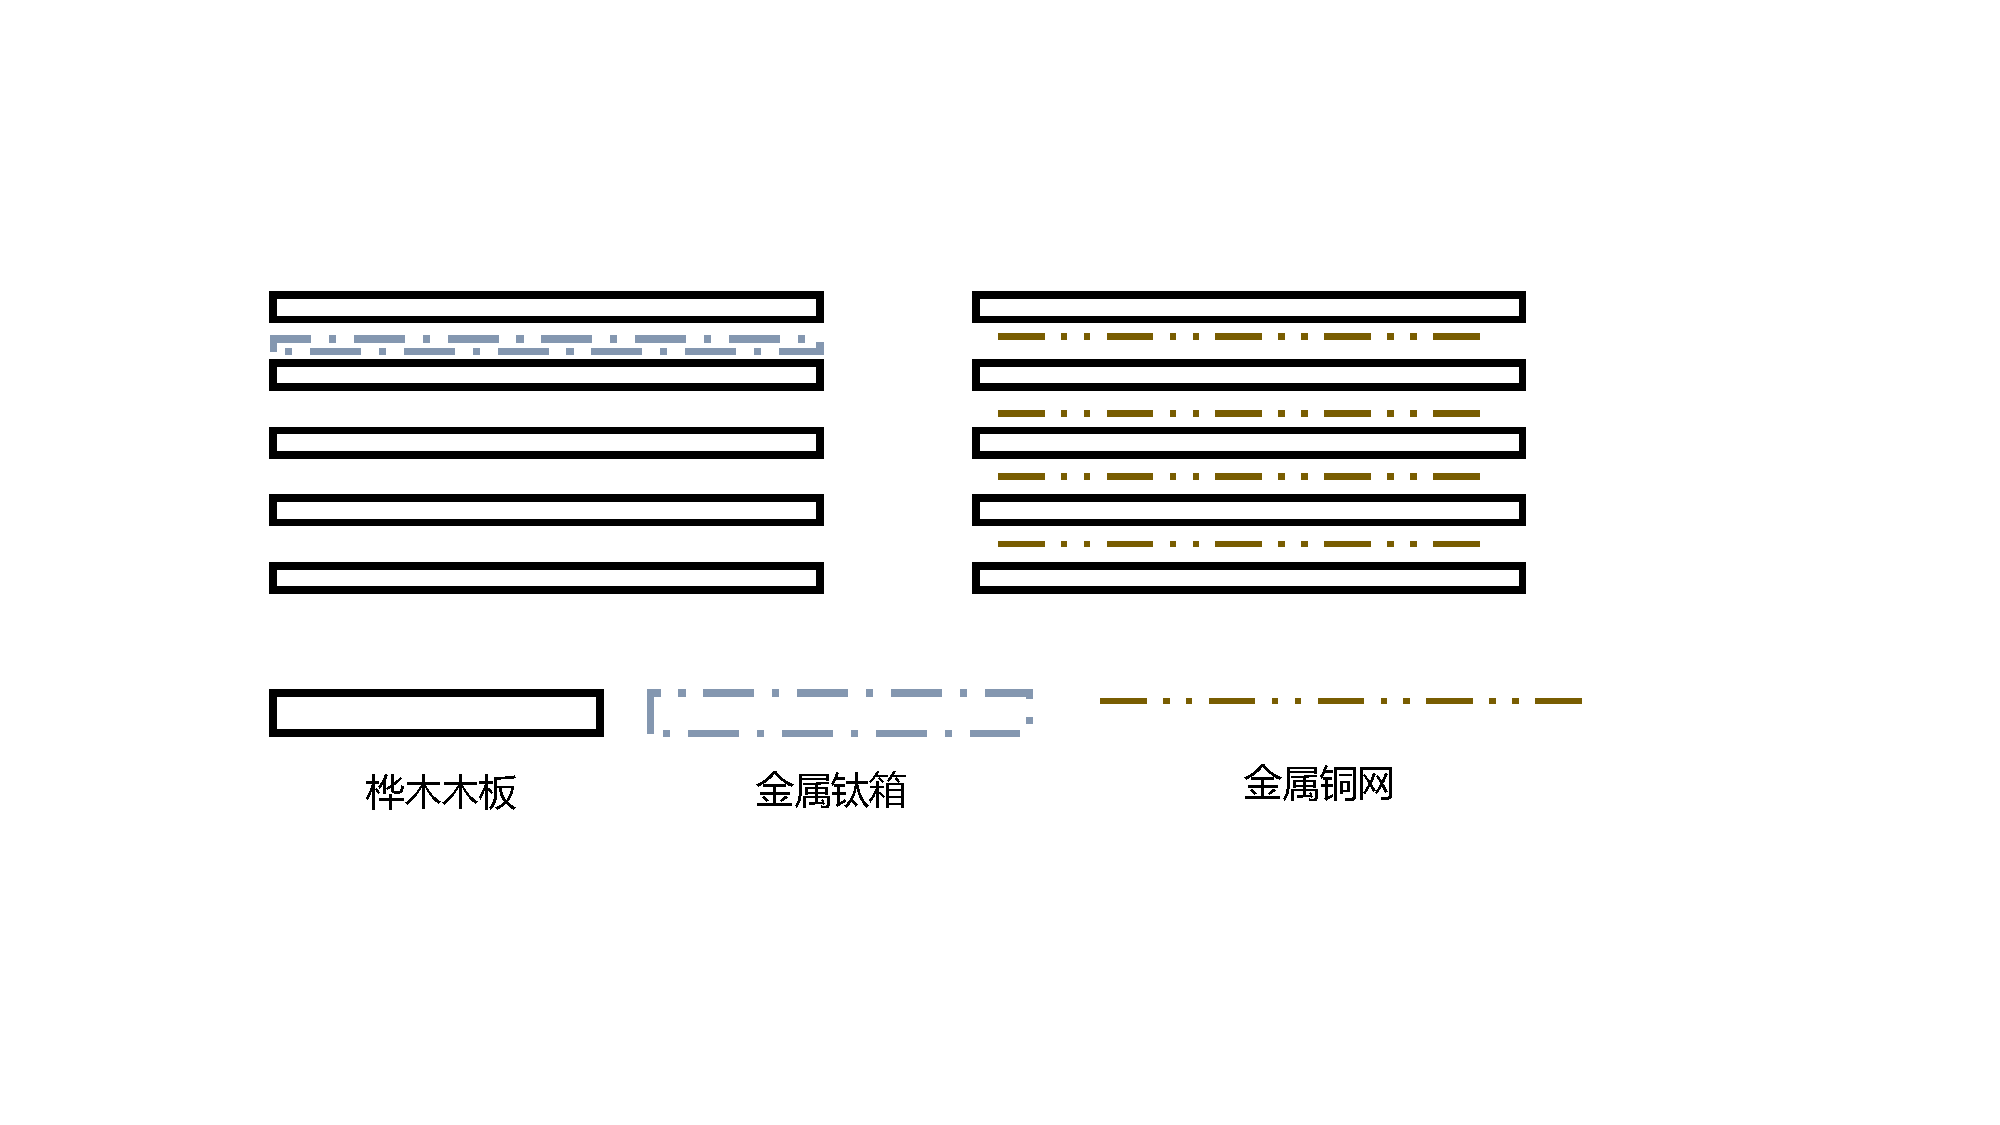
\includegraphics[width=0.5\linewidth]{CUMCMThesis-master/figures/tongwang.pdf}
    \caption{插入金属示意图}
    \label{tongwang}
\end{figure}

首先我们通过网格搜索的过程,在所要求频率[82,158,218,231,331]处,有相应的振型。再通过对图片进行傅里叶变换提取振型信息,对其内部做残差,最终选择最小残差的模型。我们不得不承认这不是一个完美的数学方法,但它切实地解决了我们的问题。最终我们得到符合要求的材料的力学参数如表~\ref{yinbancanshu}。
\begin{table}[htb]
\centering
\caption{最优音板的力学参数}
\label{table1}
\begin{tabular}{@{}cccccc@{}}
\toprule
\textbf{动弹性模量$(GPA)$}&\textbf{比动弹性模量$(GPA)$} & \textbf{密度$(kg/m^3)$} & \textbf{泊松比} \\
\midrule
16.3&20.6&860&0.2 \\
\bottomrule
\end{tabular}\label{yinbancanshu}
\end{table}

在更进一步的探究之中,传统的木材因杨氏模量与密度过小,导致固定频率过低,不能满足题目需要。使用木材与复合金属可以大幅度提高材质。通过文献调研,使用热压工艺可以达到我们需要的参数\cite{ref10}~\cite{ref11}。工艺示意图如图~\ref{tongwang},并且其最终参数整理至表~\ref{reya}~\ref{reyalixue}。
\begin{table}[htb]
\centering
\caption{不同材质的不同热压方案}
\label{table1}
\begin{tabular}{@{}ccccccc@{}}
\toprule
\textbf{热压方案名称}&\textbf{复合材质}&\textbf{施胶量$(g/cm^3)$}&\textbf{热压温度$(^\circ C)$}&\textbf{热压时间$(min)$} \\
\midrule
C1&铜&180&80&25\\
C2&铜&220&100&30\\
C3&铜&260&120&35\\
P1&钛&180&80&25\\
P2&钛&220&100&30\\
P3&钛&260&120&35\\
\bottomrule
\end{tabular}\label{reya}
\end{table}

\begin{table}[htb]
\centering
\caption{不同热压方案对应的力学参数}
\label{table1}
\begin{tabular}{@{}ccccccc@{}}
\toprule
\textbf{热压方案名称}&\textbf{动弹性模量$(GPA)$}&\textbf{比动弹性模量$(GPA)$} & \textbf{密度$(kg/m^3)$}\\
\midrule
C1&13.02&18.17&737\\
C2&15.34&20.13&762\\
C3&18.50&22.78&813\\
P1&16.71&21.05&811\\
\textbf{P2}&\textbf{16.27}&\textbf{20.07}&\textbf{842}\\
P3&16.41&20.24&810\\
\bottomrule
\end{tabular}\label{reyalixue}
\end{table}

我们得到的最优方案是P2,在此基础上最终得到的近似音板结果整理如图~\ref{last}。
\begin{figure*}[htbp]
\centering
\subfloat[吉他音板仿真82HZ]{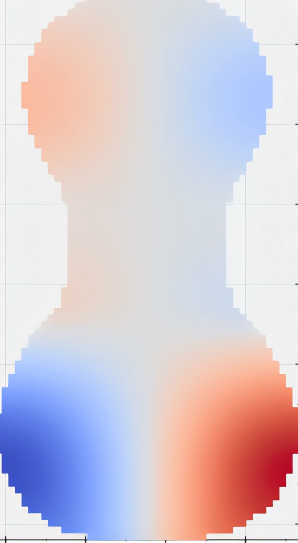
\includegraphics[width=2.5in]{CUMCMThesis-master/1.png}%
\label{fig_first_case}}
\hfil
\subfloat[吉他音板仿真331HZ]{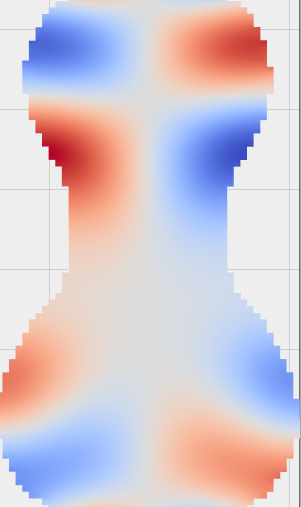
\includegraphics[width=2.5in]{CUMCMThesis-master/5.png}%
\label{fig_first_case}}
\hfil
\caption{部分吉他音板(完整版见附录~\ref{fuluB})}
\label{last}
\vspace{-0.4cm}
\label{fig10}
\end{figure*}
\section{音板振动模型敏感度分析}
在前一部分的工作之中,本文使用了复杂的方法完成题目给出的四项工作。但因动力方程不存在解析解,直接说明问题已经求解完毕是不严谨且不负责的行为,现针对本问题进行严禁且复杂的分析。
\subsection{瑞雷法求解频率偏大的原因}
在模拟仿真的过程,在问题一使用瑞雷法求解固有频率时,求解得到的结果相较于其他结果往往偏大,事实上这是瑞雷法的一个经典性质,下面将给出证明。
\begin{equation}
    W_1(\alpha,\beta)=\sum_{n=1}^\infty \sum_{m=1}^\infty a_{mn}W_{mn}(\alpha,\beta)
\end{equation}
所以瑞雷商可表示为:
\begin{equation}
   \omega^2=\frac{U\left(\sum_{n=1}^\infty \sum_{m=1}^\infty a_{mn}W_{mn}\left(\alpha,\beta\right)\right)}{\tfrac{1}{2}\iint_\delta \rho h \left(\sum_{n=1}^\infty \sum_{m=1}^\infty a_{mn}W_{mn}\left(\alpha,\beta\right)\right)^2 d s}
\end{equation}
进一步使用法式化条件可得到:
\begin{equation}
    \omega^2=\omega_{11}^2\left(\frac{a_{11}^2+a_{12}\frac{\omega_{12}^2}{\omega_{11}^2}+\dots}{a_{11}^2+a_{12}^2+a_{21}^2+\dots}\right)
\end{equation}
所以随着模态的增加,瑞雷法求解的结果会进一步偏大。
\subsection{偏微分方程解的敏感性分析}
求解微分方程的稳定性与敏感性是分析微分方程的经典步骤,薄板振动方程的稳定性问题其他工作者已经完善的十分详尽\cite{ref5},在这里就不进行更多的赘述工作。考虑到音板本身的特性,此处将对材料进行敏感性分析。

针对于低强度材料,将考虑密度在$\left[200,2000\right]kg/m^3$,弹性模量在$\left[10^8,10^9\right]kg/m^3$在$\left[0,200\right]$内的振型数量,利用振型数量判断微分方程本身的敏感性,若振型数量不随着其他属性的改变而产生大幅度改变,则低强度材料的振型相对来说较为稳定。其示意图如~\ref{Low}~所示。

可以看到,随着密度的增加,振型数量不断减少;随着弹性模量的增加,振型数量不断增加这体现了振型数量复杂度与材料强度的关系,也进一步解释图~\ref{fig_6},\ref{fig_7}~之中振型数量少于其他材料的原因。为保证分析的严谨性,接下来在更大的振型范围内,讨论高强度材料的振型数量。
\begin{figure}[H]
\centering %图片居中
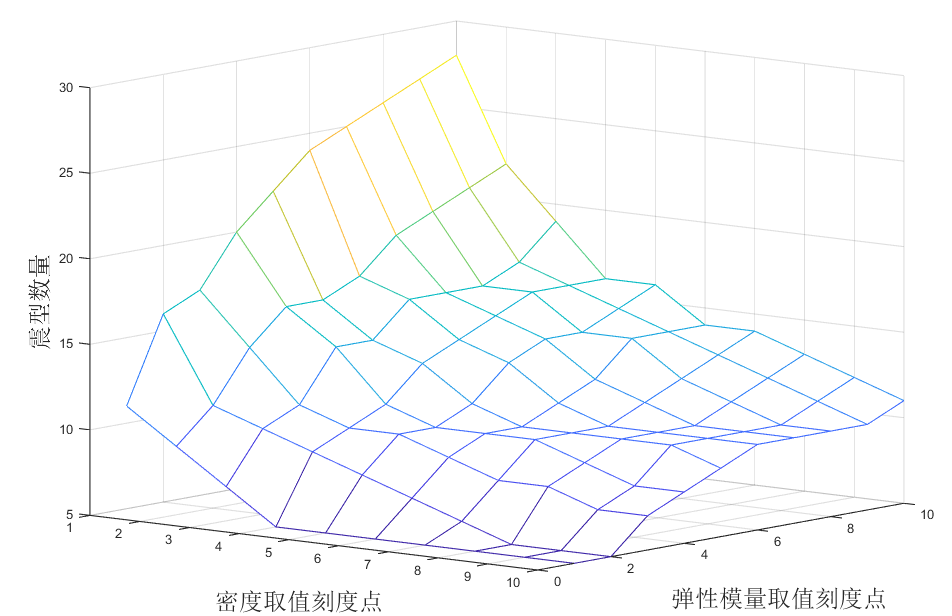
\includegraphics[width=0.6\linewidth]{CUMCMThesis-master/figures/Low.png}\caption{低强度振型分析示意图}
\label{Low}
\end{figure}

针对于高强度材料,将考虑密度在$\left[1000,10000\right]kg/m^3$,弹性模量在$\left[10^9,10^10\right]kg/m^3$在$\left[0,2000\right]$内的振型数量。其结果如图~\ref{High}~。可以看到,虽然频率范围足足扩大十倍,但高强度的不同振型数量依然远小于低强度材料振型的数量。
\begin{figure}[H]
\centering %图片居中
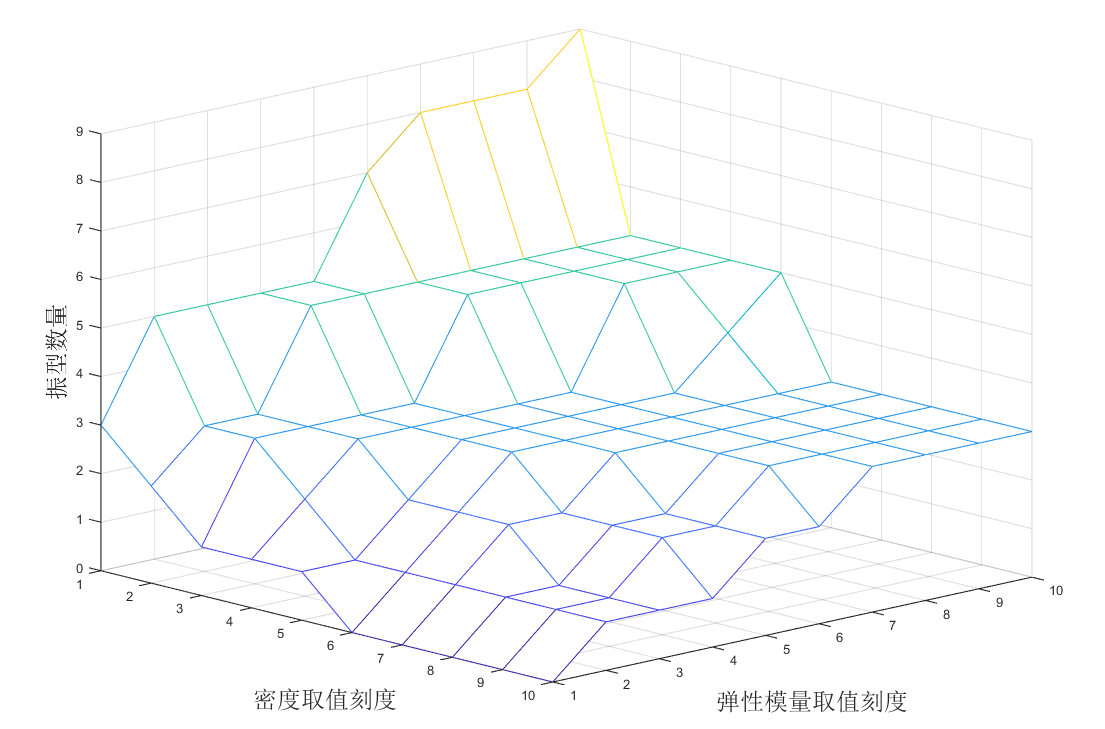
\includegraphics[width=0.6\linewidth]{CUMCMThesis-master/figures/High.png}\caption{高强度振型分析示意图}
\label{High}
\end{figure}
\subsection{振型函数拟合精准度}
在4.3节之中,本文提到在观测拟合误差图时,会出现多项式拟合的误差小于三角函数拟合的误差,但随着多项式阶数的增加,多项式的误差又会大于三角函数的误差。这是一种反直觉的现象,正常的现象应当是:随着多项式阶数的增加,模型的可解释性降低,但出现过拟合现象,精度大幅度提高。可本文之中并没有出现这种情况,通过更换求解算法,选用更适合多项式计算过程的优化算法,得到的误差图如图~\ref{newwucha}~所示。
\begin{figure}[H]
\centering %图片居中
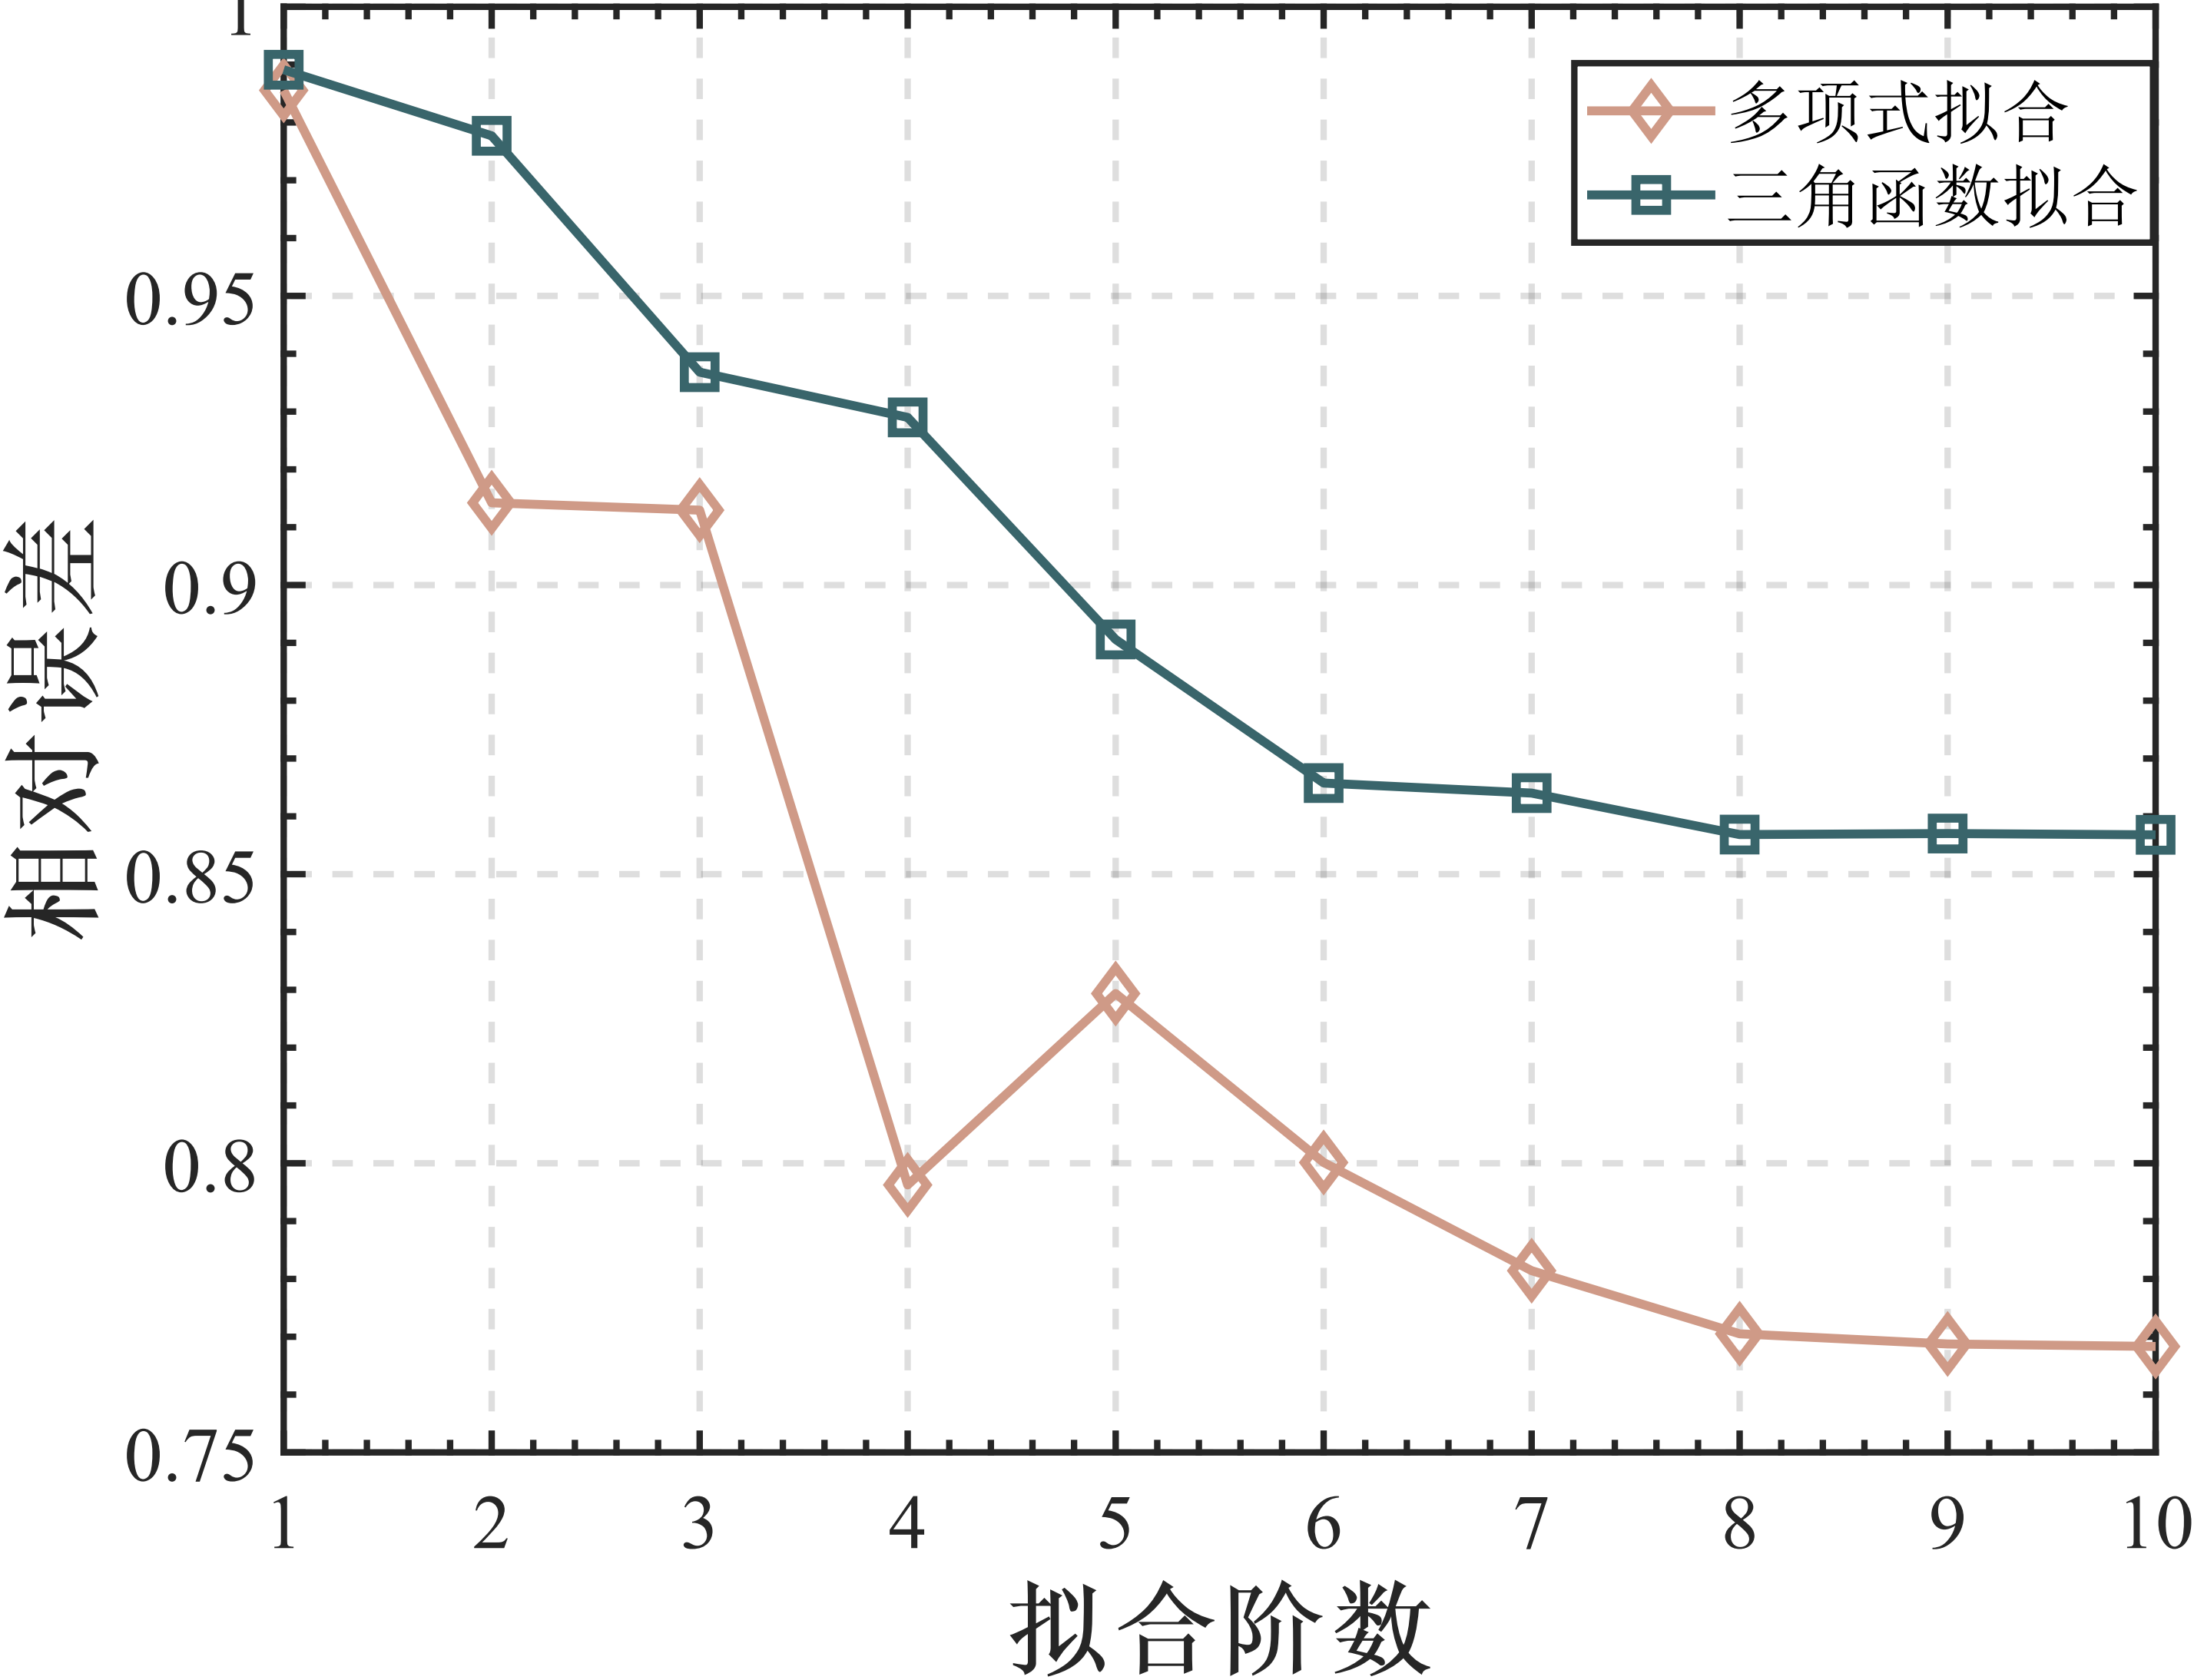
\includegraphics[width=0.6\linewidth]{CUMCMThesis-master/figures/1_1_00.png}\caption{优化算法在82HZ下的振型函数拟合误差}
\label{newwucha}
\end{figure}
图~\ref{newwucha}~表现出的结果符合基本误差拟合的方式,但这不能直接说明多项式拟合效果更好,因其内部求解参数出现$a_{ij}<10^{-9}$,此时模型可解释性极差,此时的多项式拟合效果好只是过拟合结果的体现而已。
\subsection{有限元分析问题与解决方案}
在问题二分析过程,因现有的工具箱无法使用,本文不得不建立起全新的仿真函数,但仿真函数的实际效果远不如Matlab自带的算法。

现有工具在进行特征值分解时,会选择Arnoldi算法,这是一种适用于大型稀疏矩阵的数值方法。并且为了保证得到正确的数值特征值,工程师们设计近千行的判断语句去筛选正确的特征值,这保证在均匀薄板的情况下,能够做到几乎完全正确的振动模态分析。但这些根据PDE数值分析得到的判断条件只能运用在均匀薄板的前提下。本文的非均匀模态分析无法在短时间内设置如此复杂的判别条件语句,这导致在真实的求解过程之中引入大量的无效特征值,而特征值的微小差异导致振型结果的相差巨大。

为解决这一问题,本文提供两种不同的代码结构,在已有的Matlab算法的基础上,重构计算流程得到Python的算法,Python相较于Matlab,它具有大量民间设计的可调用的分析库,而Matlab的代码用户平台分享的有限元分析的代码相对来说较为单一。调用Python的特征值求解接口,可以大幅度优化计算结果。

但很多Python的库无法通过导入的方法直接调用,在部分有限元分析软件上需要安装对应的C++程序,通过特殊的办法调用API接口;其次在一些大型的运算平台上,它因系统问题无法被正确使用,在更大型的有限元分析方案上,Matlab作为替补方案依然有着它存在价值,它无需对代码进行修改即可一键调用。附录~\ref{fuluE}~是Matlab语言下非均质薄板振动方程求解程序;附录~\ref{python}-\ref{LP}~是Python语言下非均质薄板振动方程求解程序。
\subsection{音板振动模型优缺点与后续研究展望}
本文采取基尔霍夫-洛夫动力模型将三维物体振动偏微分方程转化为二维物体振动偏微分方程模型,虽然简化问题,让求解更容易;但也导致更多的问题出现了。
\subsubsection{模型优点}
\begin{itemize}
	\item 使用基尔霍夫-洛夫动力模型,保证解的可解释性与精确性。
	\item 使用可解释性佳的三角函数振型拟合,保证模型本身的可解释性与拓展。
	\item 建立起一套完整的偏微分方程求解,振型拟合,材料拟合的工作流程,为其他工作提供理论依据。
\end{itemize}
\subsubsection{模型缺点}
\begin{itemize}
	\item 使用降维处理,导致计算过程种之中需必须使用逐点计算的方式进行仿真。虽然降低求解难度但大大增加了运算量。
	\item 没有建立更复杂的三角函数模型,以提高模型的预测精度。
	\item 没有建立起连续的材料仿真拟合,没有考虑不同材料的交界处之间需要缓冲材料粘合对振型的干扰。
\end{itemize}
\subsubsection{音板材料问题的展望与思考}
音板材料问题是一个复杂的微分方程问题,不同材料之间的融合不仅在数学方面难以解决,更在工业领域上也仅仅是刚刚开展相关研究。

在数学领域上,全新的数值求解方式可能会带来更好的模型准确度与可解释性效果。Xu.等人\cite{ref8}通过数值积分的方式得到矩形板的解析解;NGUYEN. 等人\cite{ref7}利用切比雪夫多项式构造可解析的振型函数;宋玉宇\cite{ref5}利用正交多项式里兹法构建半解析解,让模型具有数值准确度高与可解释性强的优点。这是后续研究者可以进一步参考的方式。

而在工业领域中,的吉他音板制作过程往往采用整板切割的方式,将不同材料融合整型至单板再进行切割也是复杂的物料切割控制问题,因它需要针对于不同材质的不同坐标进行切割,这需要对物料切割问题进行详细且复杂的问题分析。

音板材料问题目前仍是工业界目前没有解决的难题,随着理论与实践的不断结合,本文作者相信在不久的将来,研究者们能够通过不同材料互相融合切割的方式得到音色更加丰富优美的高质量音板。
\newpage
\begin{thebibliography}{9}%宽度9

\bibitem[1]{ref1}薛坚,牛牧青,张文勇,等.二元复合材料板的自由振动:半解析法[J].力学学报,2022,54(07):2041-2049.
\bibitem[2]{ref2}王青山,史冬岩,罗祥程.任意边界条件下矩形板的面内自由振动特性[J].华南理工大学学报(自然科学版),2015,43(06):127-134.
\bibitem[3]{ref3}朱宏祯,王纬波,殷学文,等.变厚度圆环板/圆板横向自由振动的动刚度法求解[J].应用力学学报,2019,36(06):1260-1266+1515.
\bibitem[4]{ref4}吕朋. 复杂边界条件下圆环板结构面内振动建模与特性研究[D].哈尔滨工程大学,2022.
\bibitem[5]{ref5}宋玉宇. 基于正交多项式里兹法的任意形状板自由振动研究[D].哈尔滨工程大学,2022.
\bibitem[6]{ref6}Rahbar-Ranji A, Shahbaztabar A. Free vibration analysis of non-homogeneous orthotropic plates resting on Pasternak elastic foundation by Rayleigh-Ritz method[J]. Journal of Central South University, 2016, 23(02): 413-420.
\bibitem[7]{ref7}N.D.NGUYEN, T. N. NGUYEN . Chebyshev polynomial-based Ritz method for thermal buckling and free vibration behaviors of metal foam beams[J]. Applied Mathematics and Mechanics(English Edition), 2024,45(05): 891-910.
\bibitem[8]{ref8}T. F. Xu ,Y. F. Xing. Closed-form solutions for free vibration of rectangular FGM thin plates resting on elastic foundation[J]. Acta Mechanica Sinica, 2016, 32(06): 1088-1103.
\bibitem[9]{ref9}L. SHUYU. Study the flexural vibration of rectangular thin plates with plates free boundary conditions[J]. FLEXURAL VIBRATION OF RECTANGULAR THIN PLATES WITH FREE BOUNDARY CONDITIONS, Journal of Sound and Vibration,
2001, 239, 5:1063-1071.
\bibitem[10]{ref10}郝骞,王艺达,葛颖,等.桦木单板-金属铜网复合材料声学振动性能研究[J].北京林业大学学报,2023,45(01):148-158.
\bibitem[11]{ref11}郭继龙.木质胶合板振动模态数值模拟与测试[D].中国林业科学研究院,2013.

\end{thebibliography}



%附录

\begin{appendices}


\newpage
\section{4.2节图\ref{guitarbufen}吉他型音板图像完整版} \label{fuluA}
\begin{figure*}[htbp]
\centering
\subfloat[82H下振型示意图]{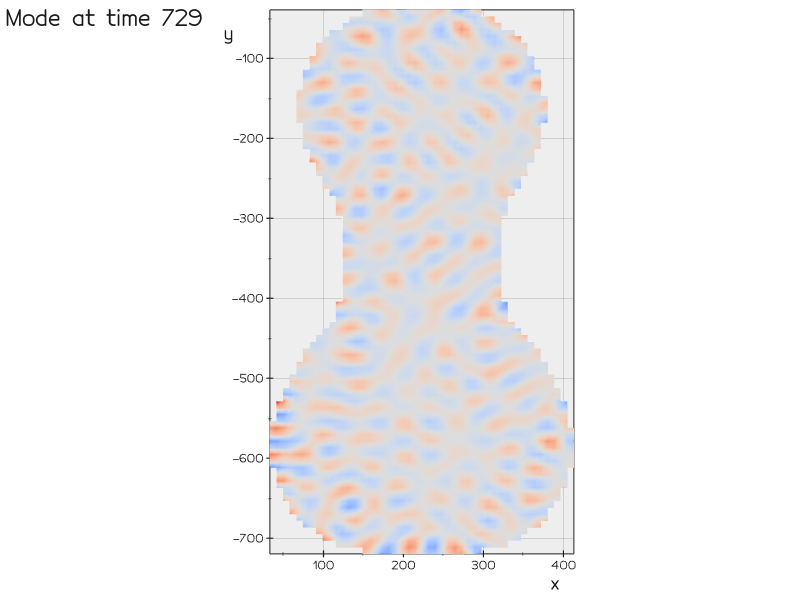
\includegraphics[width=3.1in]{CUMCMThesis-master/figures/82.png}%
\label{fig_first_case}}
\hfil
\subfloat[158HZ振型示意图]{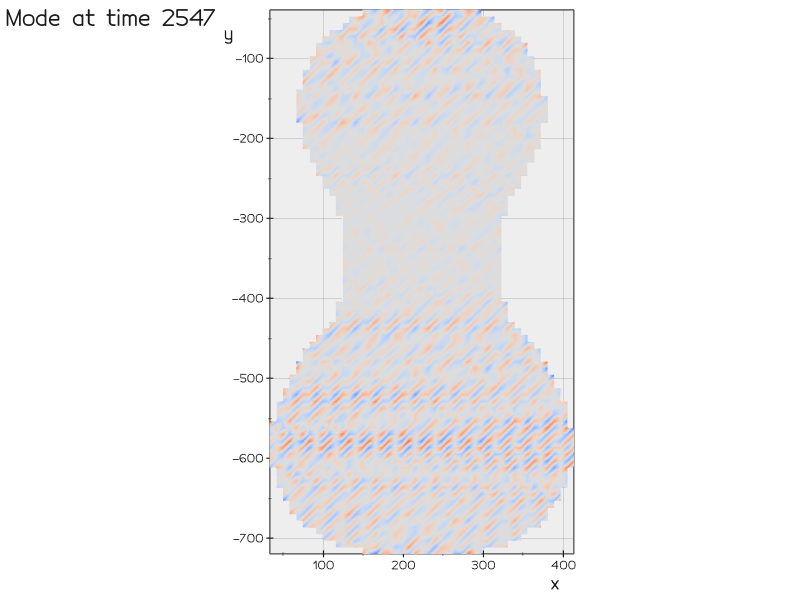
\includegraphics[width=3.1in]{CUMCMThesis-master/figures/158.png}%
\label{182}}
\hfil
\subfloat[218HZ振型示意图]{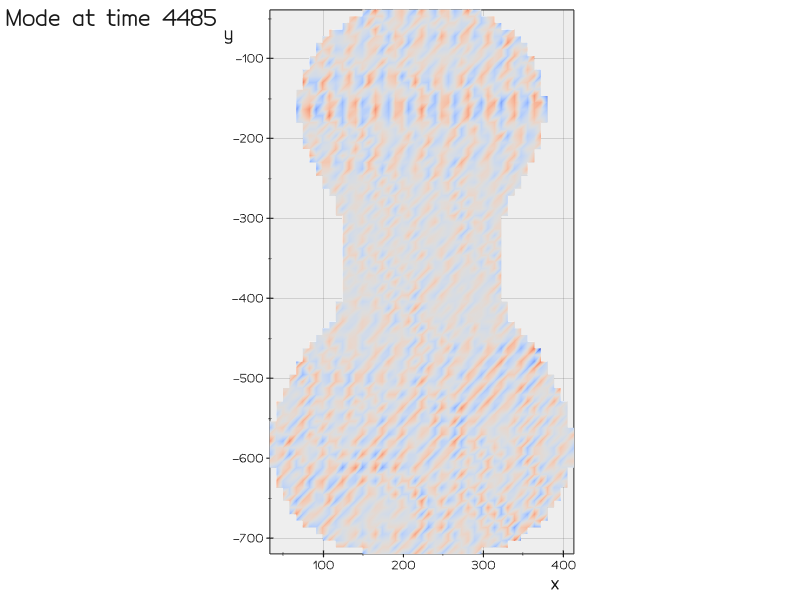
\includegraphics[width=3.1in]{CUMCMThesis-master/figures/218.png}%
\label{fig_first_case}}
\hfil
\subfloat[231HZ振型示意图]{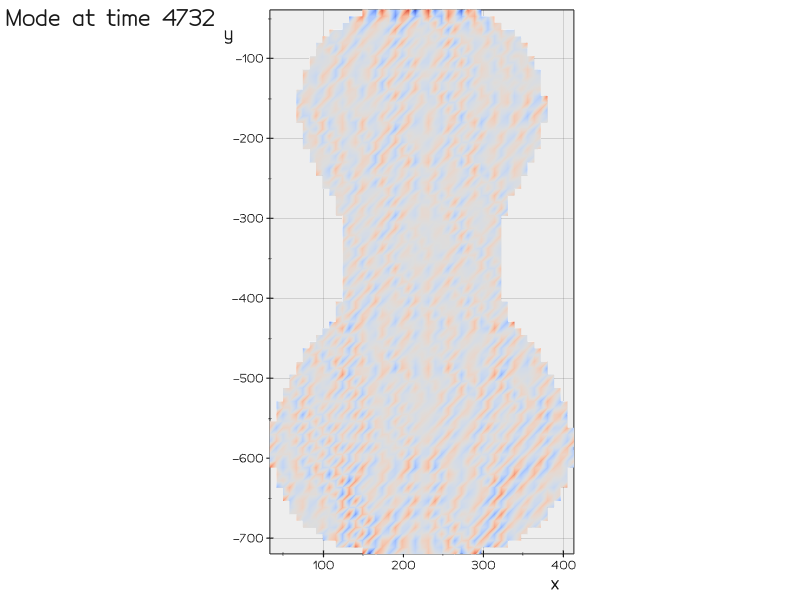
\includegraphics[width=3.1in]{CUMCMThesis-master/figures/231.png}%
\label{182}}
\hfil
\subfloat[331HZ振型示意图]{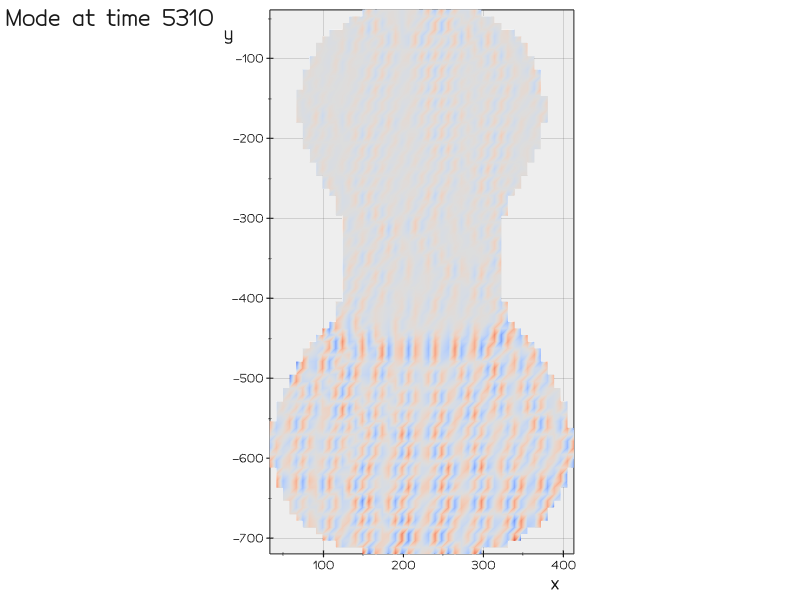
\includegraphics[width=3.1in]{CUMCMThesis-master/figures/331.png}%
\label{182}}
\hfil
\caption{吉他音板形状薄板振型示意图}
\label{fig_4.3.1}
\vspace{-0.4cm} \label{jitayinbanHZ}
\end{figure*}
\newpage

\section{4.3节图~\ref{fig_4.3.1}~振型图像完整版}\label{fuluB}
\begin{figure*}[htbp]
\centering
\subfloat[振型信息提取82HZ]{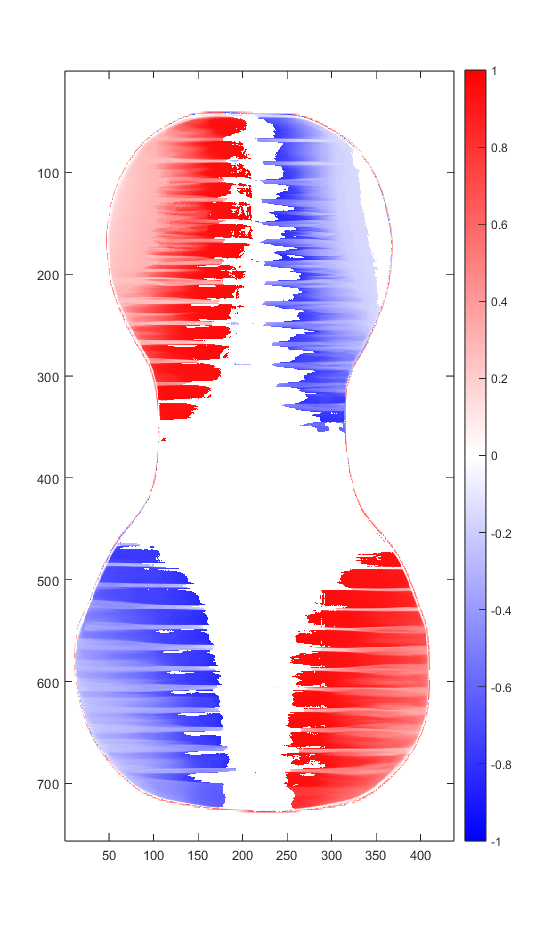
\includegraphics[width=1.3in]{CUMCMThesis-master/figures/4.3.1.png}%
\label{fig_first_case}}
\hfil
\subfloat[振兴信息提取158HZ]{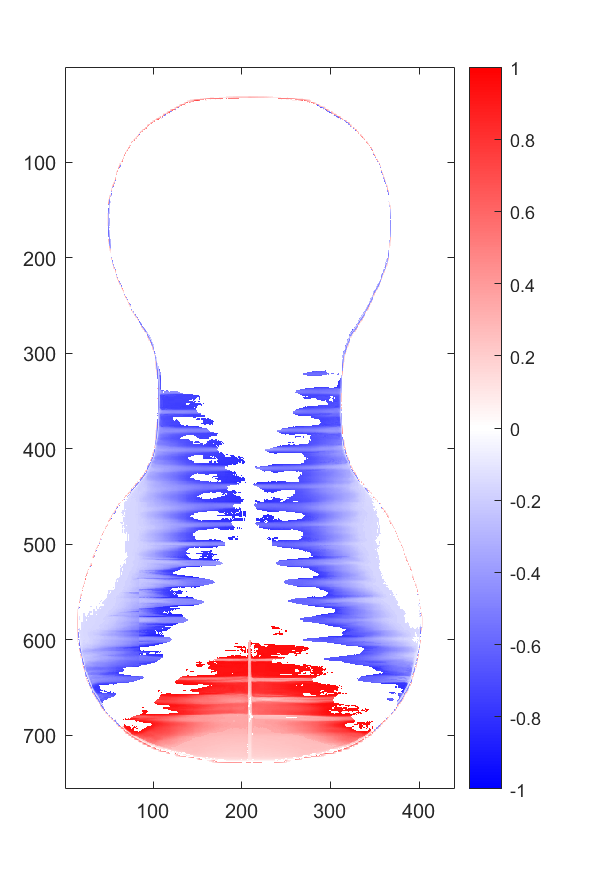
\includegraphics[width=1.3in]{CUMCMThesis-master/figures/4.3.2.png}%
\label{fig_first_case}}
\hfil
\caption{82HZ-158HZ振型信息提取}
\label{fig_4.3.1}
\vspace{-0.4cm}
\end{figure*}
\begin{figure*}[htbp]
\centering
\subfloat[振型信息提取218HZ]{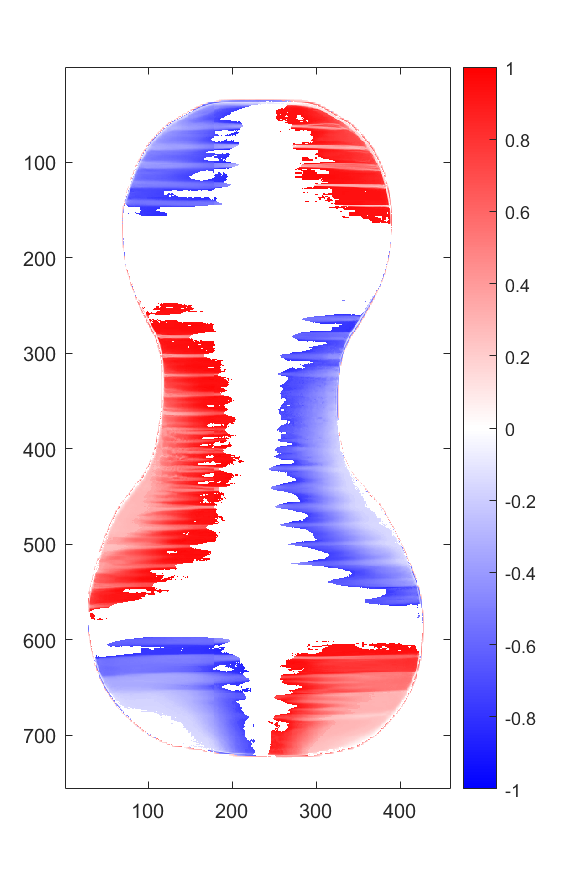
\includegraphics[width=1.3in]{CUMCMThesis-master/figures/4.3.3.png}%
\label{fig_first_case}}
\hfil
\subfloat[振型信息提取231HZ]{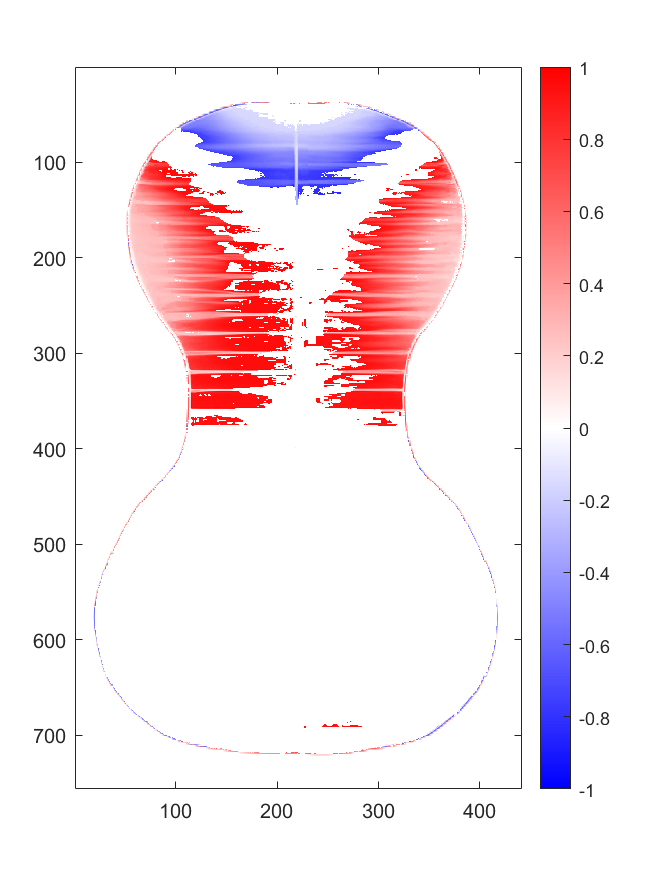
\includegraphics[width=1.3in]{CUMCMThesis-master/figures/4.3.4.png}%
\label{fig_first_case}}
\hfil
\subfloat[振型信息提取331HZ]{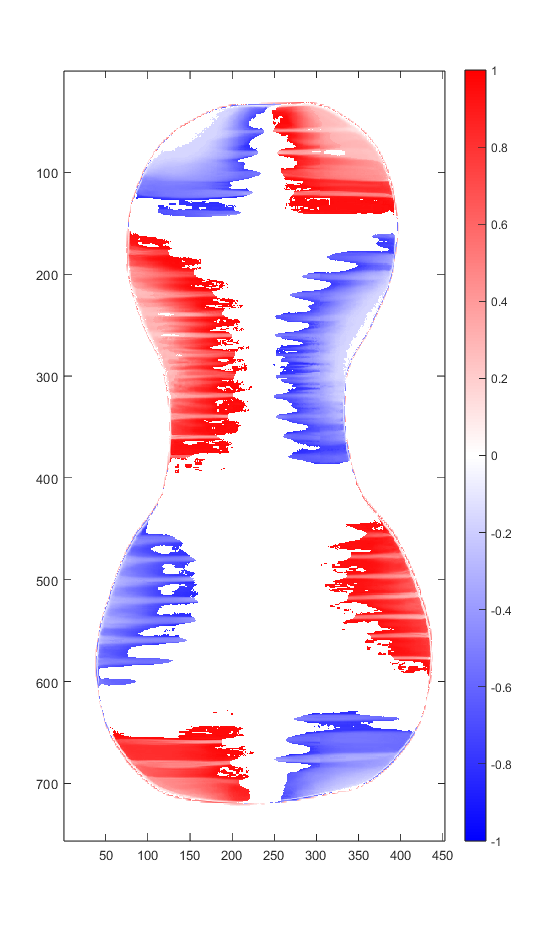
\includegraphics[width=1.3in]{CUMCMThesis-master/figures/4.3.5.png}%
\label{fig_first_case}}
\hfil
\caption{218HZ-331HZ振型信息提取}
\label{fig_4.3.1}
\vspace{-0.4cm}
\end{figure*}
\newpage
\section{4.3节图~\ref{82wucha}~振型图像完整版}\label{fuluC}
\begin{figure*}[htbp]
\centering
\subfloat[82HZ振型拟合误差图]{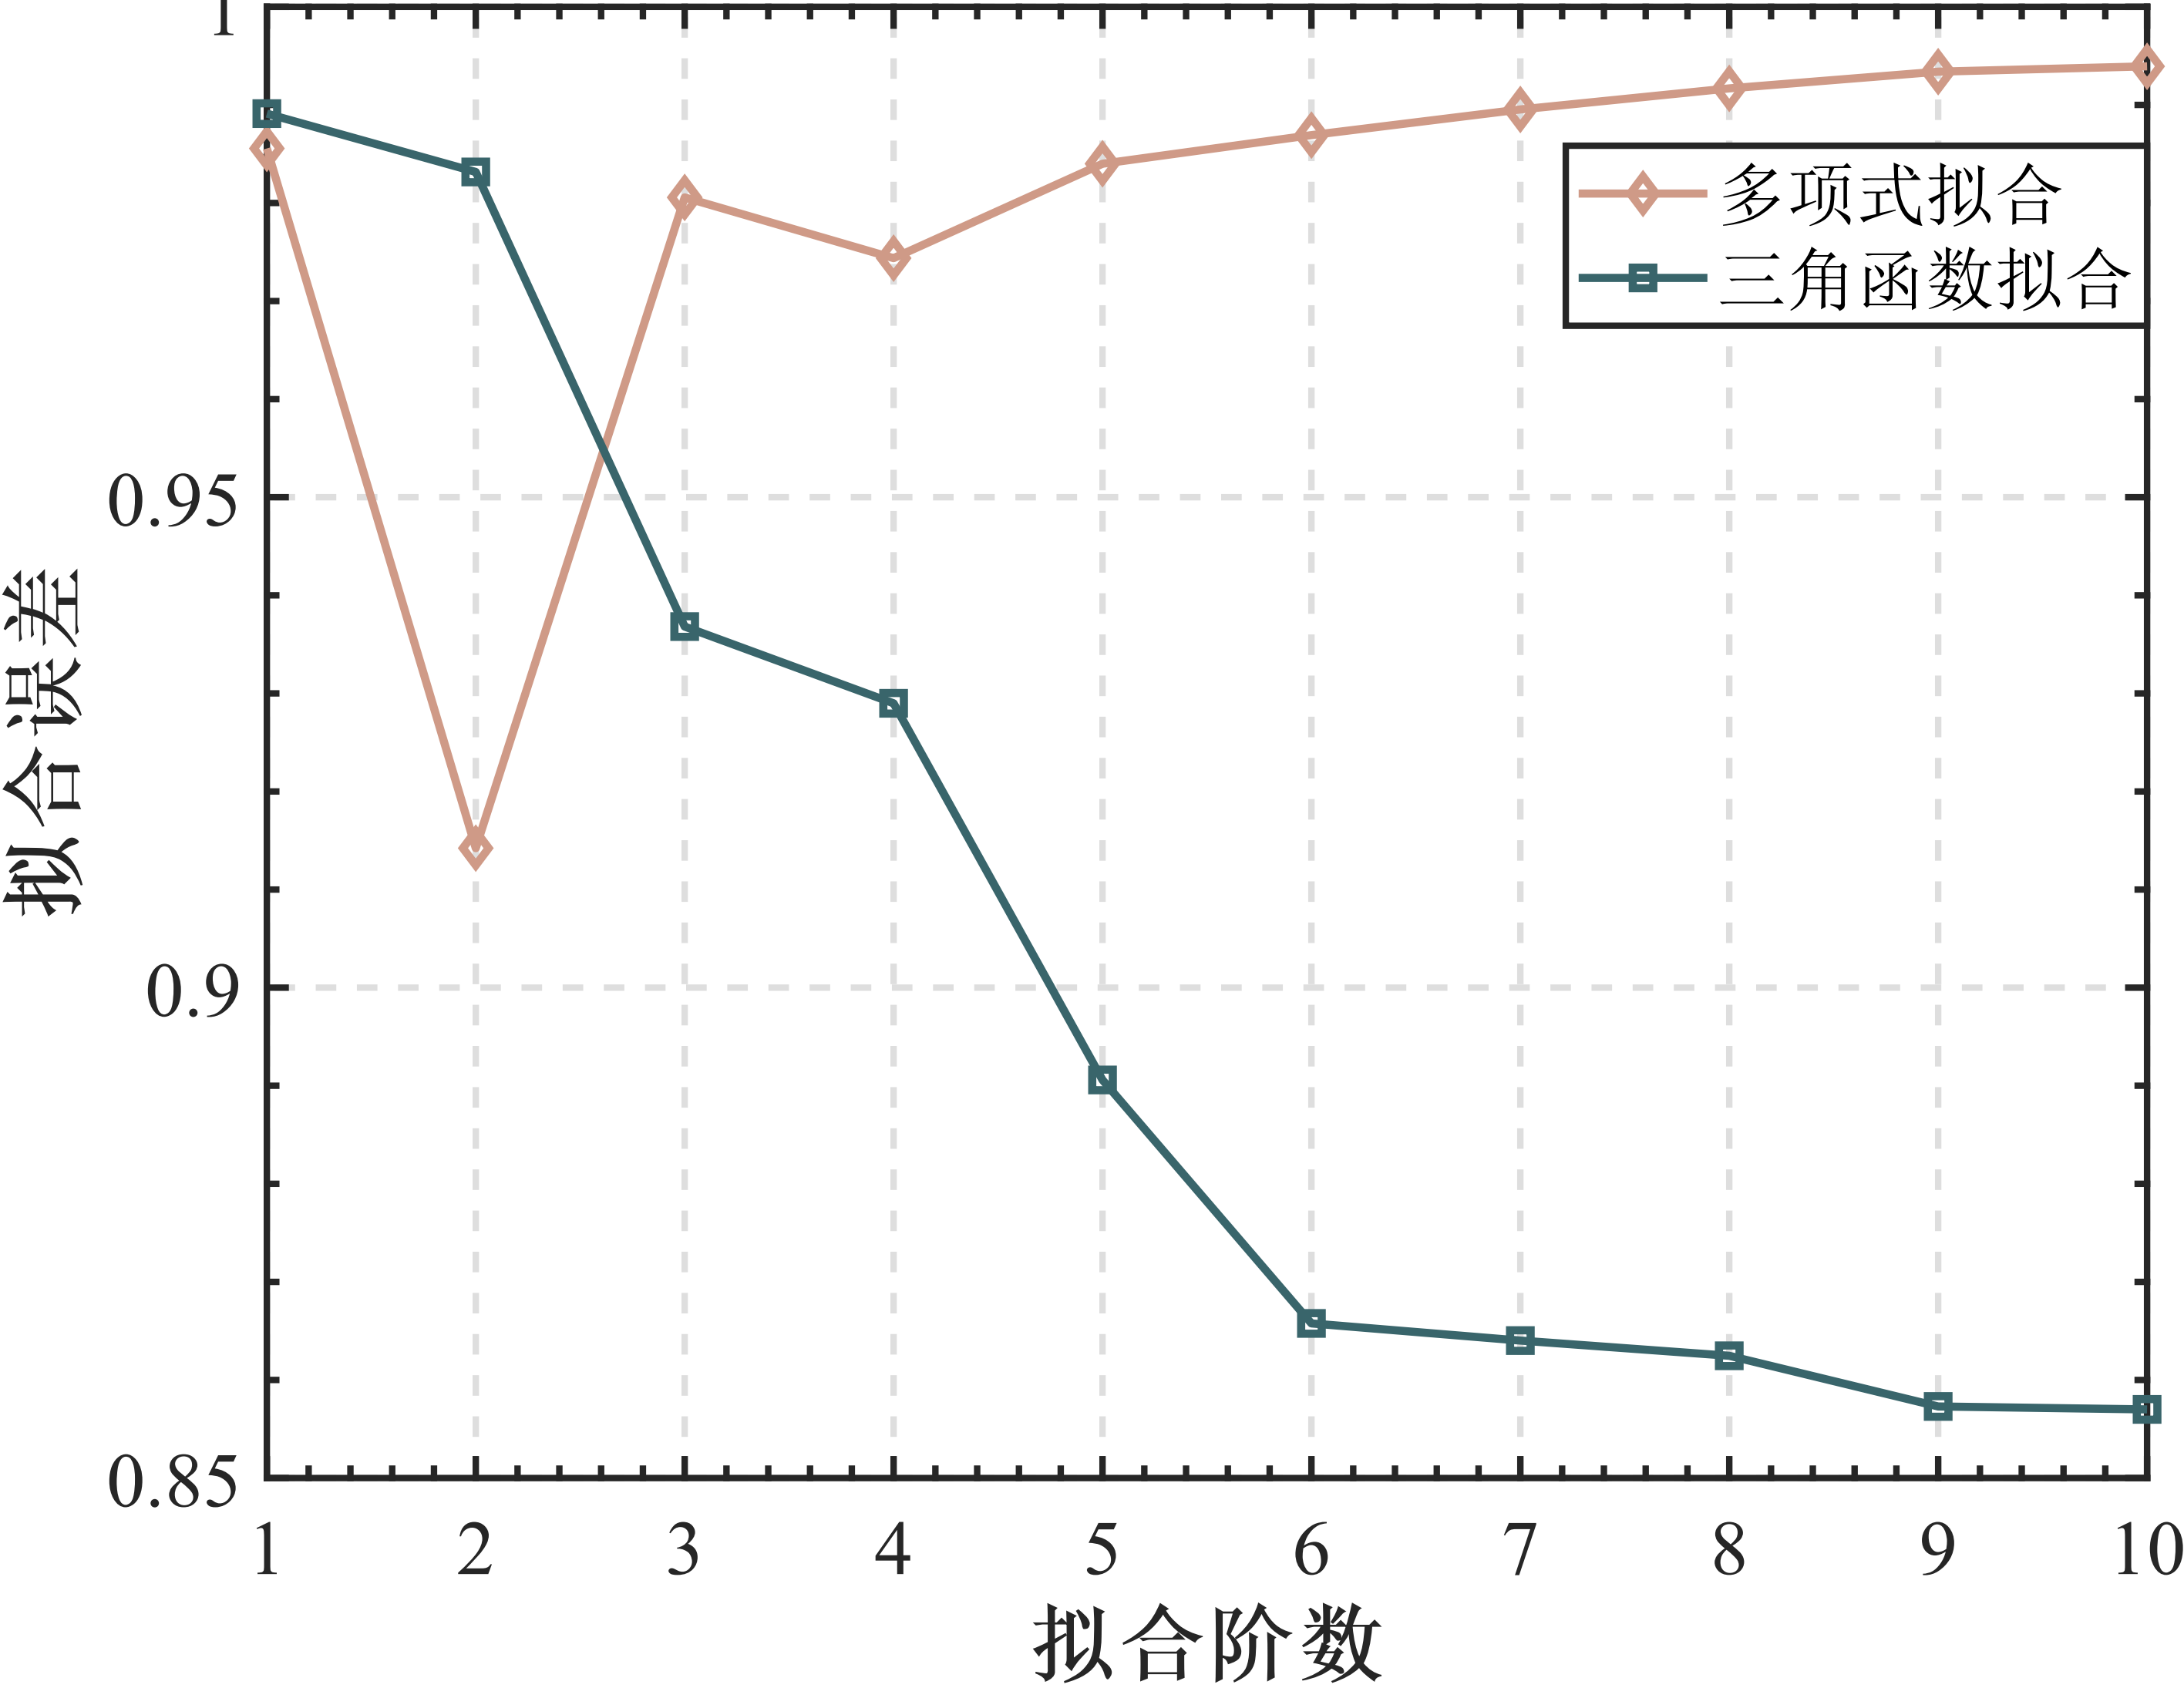
\includegraphics[width=1.3in]{CUMCMThesis-master/figures/1_00.png}%
\label{fig_first_case}}
\hfil
\subfloat[158HZ振型拟合误差图]{\includegraphics[width=1.3in]{CUMCMThesis-master/figures/2_00.png}%
\label{fig_first_case}}
\hfil
\caption{82HZ-158HZ振型拟合误差图}
\label{fig_4.3.1}
\vspace{-0.4cm}
\end{figure*}
\begin{figure*}[htbp]
\centering
\subfloat[218HZ振型拟合误差图]{\includegraphics[width=1.3in]{CUMCMThesis-master/figures/3_00.png}%
\label{fig_first_case}}
\hfil
\subfloat[231HZ振型拟合误差图]{\includegraphics[width=1.3in]{CUMCMThesis-master/figures/4_00.png}%
\label{fig_first_case}}
\hfil
\subfloat[331HZ振型拟合误差图]{\includegraphics[width=1.3in]{CUMCMThesis-master/figures/5_00.png}%
\label{fig_first_case}}
\hfil
\caption{218HZ-331HZ振型拟合误差图}
\label{fig_4.3.1}
\vspace{-0.4cm}
\end{figure*}
\newpage
\section{问题一:均质薄板振动方程求解} \label{fuluD}
\begin{lstlisting}[language=matlab]
% 1. 几何和材料属性设置
L = 1.0; 
H = 0.01; 
E = 500e9; 
nu = 0.15; 
rho = 1800; 
target_freq = 2500; 

% 2. 创建PDE模型
model = createpde('structural', 'modal-solid');

% 3. 创建立方体几何
gm = multicuboid(L, L, H);
model.Geometry = gm;
pdegplot(model, 'FaceLabels', 'on');

% 4. 设置材料属性
structuralProperties(model, 'YoungsModulus', E, ...
    'PoissonsRatio', nu, 'MassDensity', rho);

% 5. 设置边界条件
structuralBC(model, 'Face', 1:6, 'Constraint', 'free');

% 6. 设置网格
generateMesh(model, 'Hmax', 0.1 * L);

% 7. 计算自然频率
results = solve(model, 'FrequencyRange', [1 target_freq+1]);
freqs = results.NaturalFrequencies;

% 8. 显示结果
numModes = length(freqs);
fprintf('Found %d natural frequencies within the range of 0 to %d Hz\n', numModes, target_freq);
nodes = model.Mesh.Nodes; % 获取网格节点信息
for i = 1:numModes
    fprintf('Mode %d: %f Hz\n', i, freqs(i));
    figure;
    modeShapeUZ = results.ModeShapes.uz(:, i); % 获取Z方向位移数据
    % 对数据进行归一化处理
    normalizedUZ = 2 * ((modeShapeUZ - min(modeShapeUZ)) / (max(modeShapeUZ) - min(modeShapeUZ))) - 1;

    % 使用imagesc绘制标准化后的数据
    scatterX = nodes(1,:);
    scatterY = nodes(2,:);
    F = scatteredInterpolant(scatterX', scatterY', normalizedUZ, 'natural', 'none');
    [Xq, Yq] = meshgrid(linspace(min(scatterX), max(scatterX), 100), =                     linspace(min(scatterY), max(scatterY), 100));
    Vq = F(Xq, Yq);
    imagesc(Xq(1, :), Yq(:, 1), Vq);
    colormap('jet'); % 使用色谱来显示位移大小
    colorbar; % 显示色标
    xlabel('X (m)', 'FontSize', 16);
    ylabel('Y (m)', 'FontSize', 16);

    % 设置轴标签和刻度的字号
    ax = gca;
    ax.FontSize = 16; % 设置字号为20
    axis equal; % 保持坐标轴比例
end

\end{lstlisting}
\section{问题二:非均质薄板振动方程求解}\label{fuluE}
\begin{lstlisting}[language=matlab]
   % 创建 PDE 模型
    model = createpde('structural', 'modal-planestress');
    n = length(X_coords);
    shape = [2; n; X_coords; Y_coords];  % decsg 格式
    [dl, bt] = decsg(shape);
    geometryFromEdges(model, dl);
    generateMesh(model, 'Hmax', 0.1);  % 控制网格的最大单元尺寸

    % 材料属性
    E = 210e9;  % 杨氏模量(Pa)
    nu = 0.3;   % 泊松比
    % 使用mesh和位置数据计算密度
    rho = calculateDensity(model.Mesh.Nodes, Y_coords, max(Y_coords) - min(Y_coords));

    % 求解模态分析
    [K, M] = assembleGlobalMatrices(model.Mesh, E, nu, rho);

    % 计算特征值和特征向量
    [V, D] = eigs(K, M, 10,1.3426e+12);  %

    % 转换特征值为频率(根据 \lambda = \omega^2 转换)
    frequencies = sqrt(diag(D)) / (2 * pi);

    % 输出频率结果
    disp('Natural Frequencies (Hz):');
    disp(frequencies);

    for i = 1:min(10, length(frequencies))
        figure;
        modeShape = V(:, i);
        pdeplot(model, 'XYData', modeShape, 'Contour', 'on')
    end

function rho = calculateDensity(nodes, Y_coords, height)
    y_center = mean(Y_coords);
    y_grid = nodes(2, :);
    h_max = 5;
    h_min = 2;
    pixels_per_cm = max(Y_coords) / height;
    Thickness_grid = h_max - (h_max - h_min) * (((y_grid - y_center) / pixels_per_cm) / (height / 2)).^2;
    rho = 2700 * Thickness_grid / mean(Thickness_grid);  % 基于厚度的密度变化
    return
end

function [K, M] = assembleGlobalMatrices(mesh, E, nu, rho)
    numNodes = size(mesh.Nodes, 2);
    numElements = size(mesh.Elements, 2);
    K = sparse(numNodes, numNodes); % 全局刚度矩阵
    M = sparse(numNodes, numNodes); % 全局质量矩阵

    for i = 1:numElements
        nodeIndices = mesh.Elements(:, i);
        elementDensities = mean(rho(nodeIndices));  % 获取每个元素的平均密度
        nodeCoordinates = mesh.Nodes(:, nodeIndices);
        [Ke, Me] = computeElementMatrices(nodeCoordinates, E, nu, elementDensities);
        % 组装全局矩阵
        for local_i = 1:3
            for local_j = 1:3
                global_i = nodeIndices(local_i);
                global_j = nodeIndices(local_j);
                K(global_i, global_j) = K(global_i, global_j) + Ke(local_i, local_j);
                M(global_i, global_j) = M(global_i, global_j) + Me(local_i, local_j);
            end
        end
    end
    return
end
function [Ke, Me] = computeElementMatrices(nodeCoordinates, E, nu, rho)
    % 计算三角形面积
    x = nodeCoordinates(1, :);
    y = nodeCoordinates(2, :);
    area = polyarea(x, y);

    % 节点坐标局部变量
    x1 = x(1); y1 = y(1);
    x2 = x(2); y2 = y(2);
    x3 = x(3); y3 = y(3);

    % 边向量
    b = [y2 - y3, y3 - y1, y1 - y2];
    c = [x3 - x2, x1 - x3, x2 - x1];

    % 刚度矩阵 B
    B = zeros(3, 6);
    B(1, [1, 3, 5]) = b;
    B(2, [2, 4, 6]) = c;
    B(3, [1, 3, 5]) = c;
    B(3, [2, 4, 6]) = b;
    B = B / (2 * area);

    % D矩阵,平面应力情况

    D = E / (1 - nu^2) * [1, nu, 0; nu, 1, 0; 0, 0, (1 - nu) / 2];

    % 计算 Ke
    Ke = area * (B' * D * B);

    % 质量矩阵
    Me = (rho * area / 12) * [2 1 1; 1 2 1; 1 1 2];
end
\end{lstlisting}

\section{问题三:提取震动信息}
\begin{lstlisting}[language=matlab]
% 步骤1: 读取原始图像
image = imread('振型高清图1.png');  % 替换为图像的实际路径

% 步骤2: 转换到 HSV 色彩空间以提取方向信息
hsv_image = rgb2hsv(image);
hue = hsv_image(:,:,1);
saturation = hsv_image(:,:,2);
value = hsv_image(:,:,3);

warm_color_min = 0;      
warm_color_max = 60/360; 
cold_color_min = 180/360; 
cold_color_max = 240/360; 

% 创建方向映射
direction_map = zeros(size(hue));
direction_map(hue >= warm_color_min & hue <= warm_color_max) = 1;   
direction_map(hue >= cold_color_min & hue <= cold_color_max) = -1;  

% 步骤3: 将图像转换为灰度并应用方向映射
gray_image = rgb2gray(image);
amplitude = mat2gray(gray_image);
amplitude_signed = amplitude .* direction_map;

% 步骤4: 进行傅里叶变换
F = fft2(amplitude_signed);

% 步骤5: 执行傅里叶逆变换以重建原始振型
reconstructed = ifft2(F);
data = real(reconstructed);  % 取实部数据
data_normalized = (data - min(data(:))) / (max(data(:)) - min(data(:)));  % 归一化到0-1
nSteps = 128;  
positiveColorMap = [linspace(1, 1, nSteps)' linspace(1, 0, nSteps)' linspace(1, 0, nSteps)'];
negativeColorMap = [linspace(1, 0, nSteps)' linspace(1, 0, nSteps)' linspace(1, 1, nSteps)'];
cmap = [flipud(negativeColorMap); positiveColorMap];  
% 应用自定义颜色映射
figure;
imagesc(data);  
colormap(cmap);
colorbar;
caxis([-1 1]);  % 确保-1到1的数据能够覆盖整个颜色映射范围




\end{lstlisting}
\section{问题三:多项式函数拟合}
\begin{lstlisting}[language=matlab]
x_data = X(:);
y_data = Y(:);
z_data = data(:); 

% 设定多项式的最高次幂数n
n = 6;  

% 动态生成多项式模型
poly_model = @(b, xy) polyFunction(b, xy, n);

% 计算参数的数量
num_params = (n+1)*(n+2)/2;  % 每一级次数多一个参数,0次到n次

% 初始参数估计
initial_guess = zeros(num_params, 1);

% 拟合多项式模型
options = optimset('Display', 'iter'); 
params = lsqcurvefit(poly_model, initial_guess, [x_data y_data], z_data, [], [], options);

% 计算拟合后的振动数据
fitted_z_data = poly_model(params, [x_data y_data]);

% 计算误差
error = norm(z_data - fitted_z_data) / norm(z_data);
fprintf('拟合参数: ');
fprintf('%f ', params);
fprintf('\n');
fprintf('拟合误差: %f\n', error);

function z = polyFunction(b, xy, n)
    x = xy(:,1);
    y = xy(:,2);
    z = zeros(size(x));
    index = 1;
    for i = 0:n
        for j = 0:(n-i)
            z = z + b(index) * x.^i .* y.^j;
            index = index + 1;
        end
    end
end
\end{lstlisting}
\section{Python代码分析的说明文件}\label{python}
\begin{lstlisting}[language=Python]
项目名称: 非均匀薄板有限元分析问题

简介
此项目包含一组用于有限元分析和计算的脚本。每个脚本负责特定的功能,如生成网格、计算雅可比矩阵、进行模态分析等。

目录结构

├── calculate_thickness.py       # 计算厚度的脚本
├── closest_indices.py           # 找到最接近的索引的脚本
├── consistent_mass_matrix.py    # 一致质量矩阵计算脚本
├── find_closest_indices.py      # 查找最近索引的脚本
├── generate_mesh.py             # 生成网格的脚本
├── jacobian_matrix.py           # 计算雅可比矩阵的脚本
├── load_points.py               # 加载点的脚本
├── main.py                      # 主程序入口
├── modal_analysis.py            # 模态分析的脚本
├── normalize.py                 # 数据归一化的脚本
├── save_to_excel.py             # 保存结果到Excel的脚本
├── shape_function_derivatives.py# 计算形函数导数的脚本
└── stiffness_matrix.py          # 刚度矩阵计算脚本

安装和使用
1. 确保已安装 Python 3.8 或更高版本。
2. 克隆或下载此项目到本地。
3. 在项目根目录下,安装所需依赖:
4. 运行主程序:
   python main.py

文件说明
- `calculate_thickness.py`:用于计算结构厚度。
- `closest_indices.py`:找到与给定点最接近的索引。
- `consistent_mass_matrix.py`:计算一致的质量矩阵。
- `find_closest_indices.py`:查找与输入点集合最接近的索引。
- `generate_mesh.py`:生成网格数据。
- `jacobian_matrix.py`:计算雅可比矩阵。
- `load_points.py`:加载点数据。
- `main.py`:项目的主入口,调用其他模块完成整体计算。
- `modal_analysis.py`:进行模态分析。
- `normalize.py`:对数据进行归一化处理。
- `save_to_excel.py`:将计算结果保存到 Excel 文件。
- `shape_function_derivatives.py`:计算形函数的导数。
- `stiffness_matrix.py`:计算刚度矩阵。

希望这个 README 文件能帮助您更好地理解和使用此项目。如果需要进一步的帮助,请随时联系。
\end{lstlisting}
\section{Main函数}\label{python}
\begin{lstlisting}[language=Python]
import pandas as pd
import numpy as np
from vedo import shapes, Points, show, Grid, screenshot, Plotter, Mesh
from scipy.linalg import eigh
import os
import generate_mesh
import load_points
import shape_function_derivatives
import jacobian_matrix
import calculate_thickness
import consistent_mass_matrix
import stiffness_matrix
import modal_analysis
import save_to_excel
import find_closest_indices
import normalize

#主函数
def main():
    file_path = 'reduced_nodes.txt'
    points = load_points(file_path)
    points = [(x, -y) for x, y in points]
    mesh = generate_mesh(points, quads=True, jitter=0.002)
    vertices = mesh.points()
    cells = mesh.cells
    E = 2e9  # 杨氏模量,单位:Pa
    nu = 0.3  # 泊松比
    rho = 500  # 密度,单位:kg/m^3

    x_center = (np.max(vertices[:, 0]) + np.min(vertices[:, 0])) / 2
    y_center = (np.max(vertices[:, 1]) + np.min(vertices[:, 1])) / 2

    M = consistent_mass_matrix(rho, vertices, cells, x_center, y_center)
    K = stiffness_matrix(E, nu, vertices, cells, x_center, y_center)
    frequencies, modes = modal_analysis(M, K)

    # 保存频率和模态到Excel文件
    save_to_excel(frequencies, 'frequencies.xlsx')
    save_to_excel(modes, 'modes.xlsx')

    # 加载频率数据
    freq_data = pd.read_excel('frequencies.xlsx', header=None)
    freq_values = freq_data.values.flatten()

    # 目标振幅值
    target_amplitudes = [82, 158, 218, 231, 331]

    # 找到最接近的时刻
    closest_indices = find_closest_indices(freq_values, target_amplitudes)

    # 确定每个目标时刻的左右5个时刻
    all_indices = []
    for idx in closest_indices:
        for offset in range(-5, 6):
            if 0 <= idx + offset < len(freq_values):
                all_indices.append(idx + offset)

    # 去重并排序
    all_indices = sorted(set(all_indices))

    # 可视化对应时刻的琴板偏移
    for idx, time_index in enumerate(all_indices):
        mode = modes[:, time_index]
        z_values = mode[::2]

        # 归一化到最大值
        z_values = normalize(z_values)

        vertices[:, 2] = z_values

        # 创建新的Mesh对象并设置点和单元
        new_mesh = Mesh([vertices, cells])
        new_mesh.pointdata["Amplitude"] = z_values
        new_mesh.cmap("coolwarm", "Amplitude", vmin=-1, vmax=1)

        # 创建Plotter并显示
        plotter = Plotter()
        plotter.show(new_mesh, f"Mode at time {time_index}", axes=True, interactive=False)
        output_path = os.path.join(os.getcwd(), f"mode_visualization_{idx}.png")
        screenshot(output_path)
        plotter.interactive().close()
        print(f"Image saved to {output_path}")

if __name__ == "__main__":
    main()
\end{lstlisting}
\section{load$\_$points函数}
\begin{lstlisting}[language=Python]
import pandas as pd
import numpy as np
from vedo import shapes, Points, show, Grid, screenshot, Plotter, Mesh
from scipy.linalg import eigh
import os

# 从文件加载点数据
def load_points(file_path):
    points = []
    with open(file_path, 'r') as file:
        for line in file:
            parts = line.split()
            if len(parts) >= 3:
                points.append((float(parts[2]), float(parts[1])))
    return points
\end{lstlisting}
\section{modal$\_$analysis函数}
\begin{lstlisting}[language=Python]
import pandas as pd
import numpy as np
from vedo import shapes, Points, show, Grid, screenshot, Plotter, Mesh
from scipy.linalg import eigh
import os

# 模态分析
def modal_analysis(M, K):
    epsilon = 1e-6
    M += epsilon * np.eye(M.shape[0])
    eigenvalues, eigenvectors = eigh(K, M)
    frequencies = np.sqrt(eigenvalues) / (2 * np.pi)
    valid_indices = np.where((frequencies >= 0) & (frequencies <= 2000))[0]
    valid_frequencies = frequencies[valid_indices]
    valid_modes = eigenvectors[:, valid_indices]
    return valid_frequencies, valid_modes
\end{lstlisting}

\end{appendices}

\end{document} 